\documentclass[11pt]{article}

\usepackage[margin=1in]{geometry}
\usepackage{amsmath,amssymb,amsthm,mathtools}
\usepackage{enumitem}
\usepackage{hyperref}
\usepackage{tikz}
\usetikzlibrary{arrows.meta,calc,decorations.markings,decorations.pathmorphing,
  patterns,positioning,shadings,shapes.geometric,fadings,3d,backgrounds,
  intersections,shapes.misc,bending}

\allowdisplaybreaks
\setlist[enumerate]{leftmargin=*, itemsep=0.35em}

\definecolor{formblue}{HTML}{1f4e79}
\definecolor{formteal}{HTML}{0f7077}
\definecolor{formsage}{HTML}{467b3a}
\definecolor{formgold}{HTML}{b88a14}
\definecolor{formrust}{HTML}{a8431d}
\definecolor{formplum}{HTML}{6b2e6e}
\definecolor{formmauve}{HTML}{84507a}
\definecolor{formslate}{HTML}{3a5168}
\definecolor{formivory}{HTML}{f6efe0}
\definecolor{formparch}{HTML}{ece2cb}
\definecolor{windingblue}{HTML}{1f3a8a}
\newcommand{\windingnote}[1]{%
\par\smallskip
\noindent\begin{minipage}{\linewidth}%
\color{windingblue}\small%
\textbf{\textit{Winding-form thread.}}\ \textit{#1}%
\end{minipage}\par\smallskip%
}
\definecolor{handink}{HTML}{1c2e63}
\definecolor{handsepia}{HTML}{8a5a2b}
\definecolor{handpaper}{HTML}{fbf6e9}
\tikzset{
  hand/.style={
    decorate,
    decoration={random steps, segment length=2.8mm, amplitude=0.32mm},
    line cap=round, line join=round,
    draw=handink, line width=0.55pt
  },
  handthick/.style={hand, line width=0.95pt},
  handthin/.style={hand, line width=0.4pt, opacity=0.85},
  handfill/.style={hand, fill=handink!8},
  handsepia/.style={hand, draw=handsepia},
  handnote/.style={font=\itshape\scriptsize, text=handink!85!black},
  handarrow/.style={draw=handink, -{Latex[length=2.2mm]}, line width=0.7pt, line cap=round},
  handpaper/.style={fill=handpaper, draw=handink!22, line width=0.4pt, rounded corners=2pt}
}
\newcommand{\handsketch}[1]{%
\par\smallskip\noindent
\begin{minipage}{\linewidth}\centering
\begin{tikzpicture}[scale=0.78, every node/.style={font=\scriptsize}, baseline]
\useasboundingbox (-3.6,-2.0) rectangle (3.6,2.0);
#1
\end{tikzpicture}
\end{minipage}\par\smallskip%
}

\tikzset{
  vector/.style={-{Latex[length=2.2mm]}, thick},
  formarrow/.style={-{Latex[length=2mm]}, thick, blue!65!black},
  region/.style={draw=blue!60!black, fill=blue!7, thick},
  hole/.style={draw=red!70!black, fill=white, thick},
  visualnode/.style={draw=black!55, rounded corners=2pt, align=center, inner sep=5pt, fill=black!3},
  tinyarrow/.style={-{Latex[length=1.7mm]}, thick},
  flowarrow/.style={-{Latex[length=3mm,width=2.4mm,bend]}, line width=0.7pt},
  ringfade/.style={inner color=#1!28, outer color=#1!2, draw=#1!50!black, thick},
  ringfade/.default=blue,
  artpanel/.style={draw=black!22, line width=0.5pt, rounded corners=2pt,
    inner color=formivory, outer color=formivory!85!black},
  doubleformarrow/.style={-{Latex[length=2.5mm]}, line width=0.9pt, draw=formplum},
  geodesic/.style={draw=formslate, thick, opacity=0.85},
  wavyform/.style={decorate, decoration={snake, amplitude=0.45mm, segment length=2.4mm}, thick}
}
\newcommand{\visualcaption}[1]{\par\smallskip{\small\emph{#1}}\par\medskip}
\newcommand{\solutionflow}[4]{%
\begin{center}
\begin{tikzpicture}[node distance=0.75cm, every node/.style={font=\scriptsize}]
\node[visualnode, text width=2.2cm] (a) {#1};
\node[visualnode, text width=2.2cm, right=of a] (b) {#2};
\node[visualnode, text width=2.2cm, right=of b] (c) {#3};
\draw[formarrow] (a) -- (b);
\draw[formarrow] (b) -- (c);
\end{tikzpicture}
\visualcaption{#4}
\end{center}
}
\newenvironment{intentrequirements}{%
\paragraph{Intent and requirements.}
\begin{itemize}[leftmargin=*, itemsep=0.25em]
}{%
\end{itemize}
}

\newcommand{\R}{\mathbb{R}}
\newcommand{\C}{\mathbb{C}}
\newcommand{\CP}{\mathbb{CP}}
\newcommand{\dd}{\,d}
\newcommand{\pd}{\partial}
\newcommand{\Om}{\Omega}
\newcommand{\eps}{\varepsilon}

\title{Friendly Solutions to the Math 5312 / Math 7363 Midterm}
\author{}
\date{Spring 2026}

\begin{document}
\maketitle

\begin{center}
\emph{Study solutions for \texttt{Midterm\_Complex\_Analysis\_revised.pdf}. The exam instructions require handwritten submissions, so this file is intended as a reference for checking and learning the arguments.}
\end{center}

\paragraph{How to read these solutions.}
Each heading is labeled by the same problem and part number used in the exam. Within each part, the solution is written slightly more slowly than a minimal exam answer: first the relevant formula is identified, then the substitution or differentiation is carried out, and finally the result is interpreted in the language requested by the problem.

\section*{Problem 1: Differential Forms and Vector Calculus on $\R^3$}

\begin{intentrequirements}
\item \textbf{Intent.} Translate the familiar vector calculus operators into the language of differential forms and show that gradient, curl, and divergence are all appearances of the same operator $d$ in different degrees.
\item \textbf{Required outputs.} Compute $df$ for the given scalar function, identify a vector field with a $1$-form, compute $d\omega$ for a general $1$-form, compute $d\eta$ for the corresponding flux $2$-form, and summarize the full sequence
\[
 \Om^0(\R^3)\xrightarrow{d}\Om^1(\R^3)\xrightarrow{d}\Om^2(\R^3)\xrightarrow{d}\Om^3(\R^3).
\]
\item \textbf{Required explanations.} Explain which coefficient of a form corresponds to which vector component, especially the cyclic $2$-form order
\[
 dy\wedge dz,\qquad dz\wedge dx,\qquad dx\wedge dy.
\]
The solution must explicitly account for wedge-product signs such as $dy\wedge dx=-dx\wedge dy$ and for why repeated factors such as $dx\wedge dx$ vanish.
\item \textbf{Common pitfalls to avoid.} Do not read the coefficients of $d\omega$ in the visual order $dx\wedge dy$, $dy\wedge dz$, $dz\wedge dx$ when comparing with curl. The vector-field order is determined by the chosen flux-form convention.
\end{intentrequirements}

The main point of this problem is that, in Euclidean coordinates, the exterior derivative packages the three familiar vector calculus operators:
\[
 \text{grad},\qquad \text{curl},\qquad \text{div}.
\]
The only extra bookkeeping is that vector fields are identified with either $1$-forms or $2$-forms depending on which operator we want to describe.
The identifications used throughout are
\[
 (A,B,C)\longleftrightarrow A\,dx+B\,dy+C\,dz
\]
for $1$-forms, and
\[
 (A,B,C)\longleftrightarrow
 A\,dy\wedge dz+B\,dz\wedge dx+C\,dx\wedge dy
\]
for $2$-forms. The second convention is chosen so that the usual orientation
$dx\wedge dy\wedge dz$ matches the usual right-hand-rule orientation in vector calculus.

It is helpful to keep two separate ideas in mind.
\begin{enumerate}
\item The exterior derivative $d$ is a single operation defined on all differential forms.
\item The familiar vector calculus operators look different only because we identify forms with vector fields in different degrees.
\end{enumerate}
So this problem is not saying that gradient, curl, and divergence are unrelated formulas that happen to resemble $d$. It is saying that they are all the same operation $d$, written in different coordinate disguises.

\begin{center}
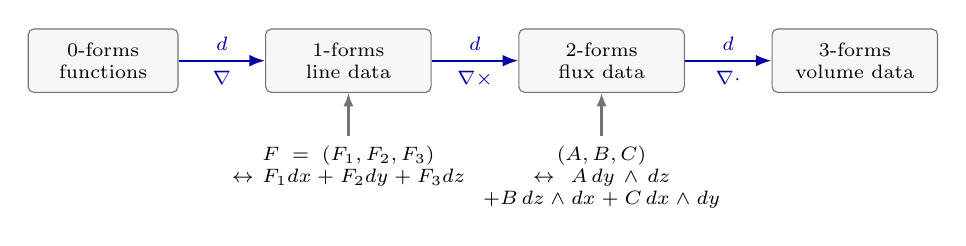
\begin{tikzpicture}[node distance=1.1cm, every node/.style={font=\scriptsize}]
\node[visualnode, text width=1.55cm] (f0) {$0$-forms\\functions};
\node[visualnode, text width=1.75cm, right=of f0] (f1) {$1$-forms\\line data};
\node[visualnode, text width=1.75cm, right=of f1] (f2) {$2$-forms\\flux data};
\node[visualnode, text width=1.75cm, right=of f2] (f3) {$3$-forms\\volume data};
\draw[formarrow] (f0) -- node[above] {$d$} node[below] {$\nabla$} (f1);
\draw[formarrow] (f1) -- node[above] {$d$} node[below] {$\nabla\times$} (f2);
\draw[formarrow] (f2) -- node[above] {$d$} node[below] {$\nabla\cdot$} (f3);
\node[below=0.55cm of f1, align=center, font=\scriptsize, text width=3.35cm] (idone)
{$F=(F_1,F_2,F_3)$\\$\leftrightarrow F_1dx+F_2dy+F_3dz$};
\node[below=0.55cm of f2, align=center, font=\scriptsize, text width=3.45cm] (idtwo)
{$(A,B,C)$\\$\leftrightarrow A\,dy\wedge dz$\\$+B\,dz\wedge dx+C\,dx\wedge dy$};
\draw[tinyarrow, black!55] (idone) -- (f1);
\draw[tinyarrow, black!55] (idtwo) -- (f2);
\end{tikzpicture}
\visualcaption{The exterior derivative is the single horizontal operation. The vector-calculus names appear after choosing the degree-dependent identification with vector fields.}
\end{center}

\paragraph{A picture gallery of the four degrees.}
The four degrees of forms on $\R^3$ correspond to four kinds of geometric data. The following gallery shows what each one ``looks like'' in coordinates: a $0$-form is a height function (here a Gaussian bump and its level lines), a $1$-form is a covector field that reads off motion along a path (depicted as a flow), a $2$-form is a flux density across oriented surfaces (depicted as an oriented face of a box), and a $3$-form is a signed volume density.

\begin{center}
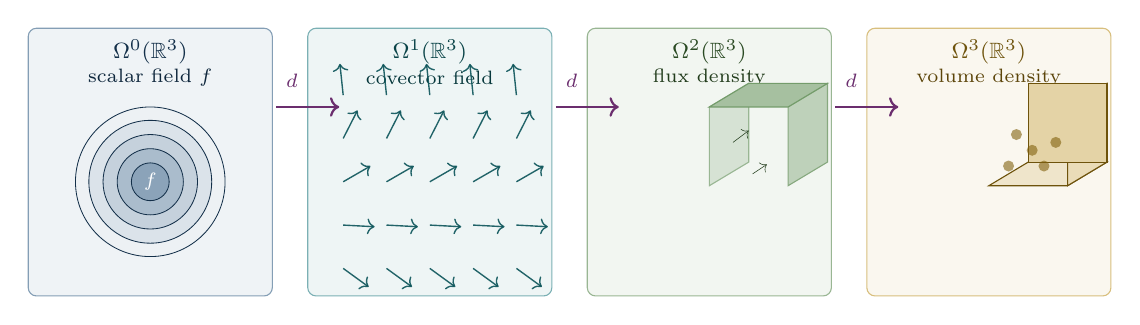
\begin{tikzpicture}[scale=1.0, every node/.style={font=\scriptsize}]
\foreach \i/\col/\tit/\sub in {0/formblue/$\Omega^0(\R^3)$/scalar field $f$,1/formteal/$\Omega^1(\R^3)$/covector field,2/formsage/$\Omega^2(\R^3)$/flux density,3/formgold/$\Omega^3(\R^3)$/volume density}{
  \begin{scope}[xshift=\i*3.55cm]
    \filldraw[draw=\col!55, fill=\col!7, rounded corners=3pt, line width=0.4pt]
      (-1.55,-1.55) rectangle (1.55,1.85);
    \node[\col!60!black, font=\bfseries\footnotesize] at (0,1.55) {\tit};
    \node[\col!50!black, font=\scriptsize] at (0,1.22) {\sub};
  \end{scope}
}
% 0-form: contour plot of a bump
\begin{scope}[xshift=0cm, yshift=-0.1cm]
  \foreach \r/\op in {0.95/8,0.78/16,0.6/26,0.42/38,0.24/52}
    \filldraw[draw=formblue!60!black, fill=formblue!\op, line width=0.3pt] (0,0) circle (\r);
  \node[white, font=\scriptsize] at (0,0) {$f$};
\end{scope}
% 1-form: flow field
\begin{scope}[xshift=3.55cm, yshift=-0.1cm]
  \foreach \x in {-1.1,-0.55,0,0.55,1.1}{
    \foreach \y in {-1.1,-0.55,0,0.55,1.1}{
      \draw[->, formteal!75!black, line width=0.5pt, opacity=0.9] (\x,\y) -- ++({0.4*cos(60*\y+30)},{0.4*sin(60*\y+30)});
    }
  }
\end{scope}
% 2-form: oriented faces of a cube
\begin{scope}[xshift=7.1cm, yshift=-0.15cm]
  \coordinate (O) at (0,0);
  \coordinate (X) at (1.0,0);
  \coordinate (Y) at (0.5,0.3);
  \coordinate (Z) at (0,1.0);
  \filldraw[draw=formsage!55, fill=formsage!22, line width=0.4pt]
    (O) -- (Y) -- ($(Y)+(Z)$) -- (Z) -- cycle;
  \filldraw[draw=formsage!65, fill=formsage!35, line width=0.4pt]
    (X) -- ($(X)+(Y)$) -- ($(X)+(Y)+(Z)$) -- ($(X)+(Z)$) -- cycle;
  \filldraw[draw=formsage!75, fill=formsage!48, line width=0.4pt]
    ($(Z)$) -- ($(Z)+(X)$) -- ($(Z)+(X)+(Y)$) -- ($(Z)+(Y)$) -- cycle;
  \draw[->, formsage!50!black, very thin] (0.3,0.55) -- ++(0.2,0.15);
  \draw[->, formsage!50!black, very thin] (0.55,0.15) -- ++(0.18,0.12);
\end{scope}
% 3-form: volume density (3D-ish cube)
\begin{scope}[xshift=10.65cm, yshift=-0.15cm]
  \coordinate (O) at (0,0);
  \coordinate (X) at (1.0,0);
  \coordinate (Y) at (0.5,0.3);
  \coordinate (Z) at (0,1.0);
  \filldraw[draw=formgold!60!black, fill=formgold!22, line width=0.4pt]
    (O) -- (X) -- ($(X)+(Y)$) -- (Y) -- cycle;
  \filldraw[draw=formgold!60!black, fill=formgold!30, line width=0.4pt]
    (X) -- ($(X)+(Y)$) -- ($(X)+(Y)+(Z)$) -- ($(X)+(Z)$) -- cycle;
  \filldraw[draw=formgold!60!black, fill=formgold!38, line width=0.4pt]
    (Y) -- ($(X)+(Y)$) -- ($(X)+(Y)+(Z)$) -- ($(Y)+(Z)$) -- cycle;
  % density pattern inside
  \foreach \p in {(0.25,0.25),(0.55,0.45),(0.35,0.65),(0.7,0.25),(0.85,0.55)}
    \fill[formgold!70!black, opacity=0.6] \p circle (0.07);
\end{scope}
% Arrows between panels
\foreach \i in {0,1,2}{
  \pgfmathsetmacro\x{(\i+1)*3.55-1.55}
  \pgfmathsetmacro\xx{(\i+1)*3.55-1.95}
  \draw[->, formplum, line width=0.8pt] (\xx,0.85) -- (\x+0.4,0.85);
  \node[formplum, font=\scriptsize] at (\xx+0.2,1.18) {$d$};
}
\end{tikzpicture}
\visualcaption{Each degree of form encodes a distinct geometric content. The operator $d$ moves consistently across the four panels and, after the metric identifications, recovers $\nabla,\nabla\times,\nabla\cdot$ as a single uniform rule.}
\end{center}

\windingnote{The exterior derivative $d$ takes closed forms (those satisfying $d\omega=0$) and asks whether they are exact (i.e., equal $d\eta$ for some $\eta$). On $\R^3$ the answer is always yes (Poincar\'e lemma), and the de Rham complex above has no $H^1$. The canonical example refuting this on a non-simply-connected domain is the \emph{winding $1$-form} $\omega=\frac{-y\,dx+x\,dy}{x^2+y^2}$ on $\R^2\setminus\{0\}$, which Problem~2 studies in full. A direct computation gives $d\omega=0$, so $\omega$ \emph{is} closed; yet $\oint_{S^1}\omega=2\pi\neq 0$, so $\omega$ cannot be the differential of any globally defined function (the candidate function would be the angle $\theta$, which is multi-valued). This single example is the seed of de Rham cohomology in degree~$1$ and of every ``residue-style'' obstruction that follows in Problems~$3$, $5$, and $9$.}

\handsketch{%
\fill[handpaper] (-3.4,-1.85) rectangle (3.4,1.85);
\draw[hand] (-3.4,-1.85) rectangle (3.4,1.85);
% Hole at origin
\draw[handthick] (0,0) circle (0.18);
\node[handnote] at (0,-0.4) {puncture};
% Spiraling tangent field around 0
\foreach \th in {15,55,...,355}{
  \draw[handarrow] (\th:1.0) -- ++({\th+90}:0.55);
}
\foreach \th in {25,65,...,345}{
  \draw[hand, line width=0.35pt, opacity=0.7] (\th:1.7) -- ++({\th+90}:0.4);
}
% A loop around 0
\draw[handthick] (0,0) circle (1.95);
\draw[handarrow] (40:1.95) arc (40:120:1.95);
% labels
\node[handnote] at (2.6,1.6) {$\omega=\dfrac{-y\,dx+x\,dy}{x^{2}+y^{2}}$};
\node[handnote] at (2.6,1.0) {$d\omega=0$};
\node[handnote] at (2.6,0.6) {$\oint\omega=2\pi$};
\node[handnote] at (-2.5,-1.45) {closed, not exact};
}

\subsection*{Problem 1(a): Gradient and $1$-forms}

\solutionflow{function\\\(f=x^2y+yz^2\)}
{partial derivatives\\\(\pd_x f,\pd_y f,\pd_z f\)}
{\(df\) coefficients\\match \(\nabla f\)}
{Problem 1(a) is solved by reading the three partial derivatives simultaneously as differential-form coefficients and as gradient components.}

Throughout Problem 1(a) we work with the scalar function
\[
 f(x,y,z)=x^2y+yz^2.
\]

\subsubsection*{Problem 1(a)-1: Compute the exterior derivative $df$}

Compute the three partial derivatives:
\[
 \pd_x f=2xy,\qquad
 \pd_y f=x^2+z^2,\qquad
 \pd_z f=2yz.
\]
By the definition $df=\pd_x f\,dx+\pd_y f\,dy+\pd_z f\,dz$,
\[
 df=2xy\,dx+(x^2+z^2)\,dy+2yz\,dz.
\]

\subsubsection*{Problem 1(a)-2: Compute the gradient vector field $\nabla f$}

The gradient is the vector field whose components are the same partial derivatives:
\[
 \nabla f=(\pd_x f,\;\pd_y f,\;\pd_z f)=(2xy,\;x^2+z^2,\;2yz).
\]

\subsubsection*{Problem 1(a)-3: Coefficients of $df$ correspond to components of $\nabla f$}

The coefficient of $dx$ in $df$ is the first component of $\nabla f$, the coefficient of $dy$ is the second component, and the coefficient of $dz$ is the third component. In other words,
\[
 df=(\nabla f)_1\,dx+(\nabla f)_2\,dy+(\nabla f)_3\,dz.
\]
For this specific function the comparison is
\[
\begin{array}{c|c|c}
\text{basis form} & \text{coefficient in }df & \text{component of }\nabla f\\ \hline
dx & 2xy & 2xy\\
dy & x^2+z^2 & x^2+z^2\\
dz & 2yz & 2yz
\end{array}
\]

\subsubsection*{Problem 1(a)-4: Correspondence between $\Omega^0(\R^3)$ and $\Omega^1(\R^3)$}

By the previous step, applying $d$ to a $0$-form (a function) produces a $1$-form whose three coefficients are exactly the components of the gradient vector field. So the exterior derivative
\[
 d:\Om^0(\R^3)\longrightarrow \Om^1(\R^3)
\]
is the differential-form version of the gradient map
\[
 f\longmapsto \nabla f.
\]
This is a correspondence of operators: a function becomes its differential $df$, and the same three coefficient functions form the vector field $\nabla f$.

Strictly speaking, $d:\Om^0(\R^3)\to\Om^1(\R^3)$ is not surjective onto all $1$-forms: only \emph{closed} $1$-forms can be exterior derivatives. On $\R^3$ the Poincar\'e lemma says closed implies exact, so the image of $d$ on $0$-forms is exactly the closed $1$-forms (equivalently, the curl-free vector fields). On a non-simply-connected domain such as $\R^2\setminus\{0\}$ (Problem~2), even closed $1$-forms need not be exact, and that cohomological obstruction is one of the things de Rham theory measures. The point here is that the operation ``take exterior derivative of a $0$-form'' is the form-language version of ``take the gradient,'' and that the identification
\[
 (A,B,C)\longleftrightarrow A\,dx+B\,dy+C\,dz
\]
turns vector fields on $\R^3$ into $1$-forms. Under this identification, $\nabla f$ corresponds to $df$.

\subsection*{Problem 1(b): Vector fields and $1$-forms}

\solutionflow{vector field\\\(F=(F_1,F_2,F_3)\)}
{lower index\\using Euclidean metric}
{\(1\)-form\\\(F_1dx+F_2dy+F_3dz\)}
{Problem 1(b) is the metric identification between vectors and covectors in standard Euclidean coordinates.}

Throughout Problem 1(b) we work with a vector field
\[
 F=(F_1,F_2,F_3)
\]
on $\R^3$ with smooth components.

\subsubsection*{Problem 1(b)-1: Construct the corresponding $1$-form}

The corresponding $1$-form is
\[
 \omega=F_1\,dx+F_2\,dy+F_3\,dz.
\]
Concretely, the construction takes the three component functions of $F$ and uses them as the coefficients of the standard basis $1$-forms $dx,dy,dz$.

\subsubsection*{Problem 1(b)-2: One-to-one correspondence between vector fields and $1$-forms}

Conversely, any $1$-form
\[
 \omega=a\,dx+b\,dy+c\,dz
\]
determines the vector field
\[
 F=(a,b,c).
\]
The map
\[
 (F_1,F_2,F_3)
 \longmapsto
 F_1\,dx+F_2\,dy+F_3\,dz
\]
and its inverse, which reads off the coefficients, are mutually inverse. Hence, in the standard Euclidean coordinates, vector fields on $\R^3$ are in one-to-one correspondence with $1$-forms.

The phrase ``standard Euclidean coordinates'' matters because we are using the usual dot product to identify vectors and covectors. In more geometric language, the Euclidean metric turns the vector field $F$ into the covector field $\omega$ by lowering an index.

Concretely, if $v=(v_1,v_2,v_3)$ is a tangent vector at a point, then
\[
 \omega(v)=F_1v_1+F_2v_2+F_3v_3=F\cdot v.
\]
So the $1$-form $\omega$ is the object that eats a tangent vector and returns the dot product with $F$. This is why line integrals of vector fields and line integrals of $1$-forms are the same calculation in Euclidean space.

\subsection*{Problem 1(c): Curl and $2$-forms}

\solutionflow{\(1\)-form\\\(\omega=F_1dx+F_2dy+F_3dz\)}
{differentiate\\and collect wedges}
{\(2\)-form coefficients\\are \(\nabla\times F\)}
{Problem 1(c) is solved by collecting the surviving wedge terms and then reading them in cyclic face order.}

Throughout Problem 1(c) we work with a vector field
\[
 F=(F_1,F_2,F_3)
\]
and the associated $1$-form
\[
 \omega=F_1\,dx+F_2\,dy+F_3\,dz.
\]

\subsubsection*{Problem 1(c)-1: Compute the exterior derivative $d\omega$}

We expand $d\omega$ one term at a time:
\[
 d\omega=d(F_1\,dx)+d(F_2\,dy)+d(F_3\,dz).
\]
Since $d(dx)=d(dy)=d(dz)=0$, this becomes
\[
 d\omega=dF_1\wedge dx+dF_2\wedge dy+dF_3\wedge dz.
\]
Now
\[
 dF_1=(\pd_xF_1)dx+(\pd_yF_1)dy+(\pd_zF_1)dz,
\]
so
\[
\begin{aligned}
 dF_1\wedge dx
 &=(\pd_xF_1)dx\wedge dx+(\pd_yF_1)dy\wedge dx+(\pd_zF_1)dz\wedge dx\\
 &=-\pd_yF_1\,dx\wedge dy+\pd_zF_1\,dz\wedge dx.
\end{aligned}
\]
Similarly,
\[
\begin{aligned}
 dF_2\wedge dy
 &=(\pd_xF_2)dx\wedge dy+(\pd_yF_2)dy\wedge dy+(\pd_zF_2)dz\wedge dy\\
 &=\pd_xF_2\,dx\wedge dy-\pd_zF_2\,dy\wedge dz,
\end{aligned}
\]
and
\[
\begin{aligned}
 dF_3\wedge dz
 &=(\pd_xF_3)dx\wedge dz+(\pd_yF_3)dy\wedge dz+(\pd_zF_3)dz\wedge dz\\
 &=-\pd_xF_3\,dz\wedge dx+\pd_yF_3\,dy\wedge dz.
\end{aligned}
\]
Collecting the coefficients of the three standard $2$-forms gives the formula below.
Using the formula for the exterior derivative of a $1$-form,
\[
\begin{aligned}
 d\omega
 &=(\pd_xF_2-\pd_yF_1)\,dx\wedge dy  \\
 &\quad+(\pd_yF_3-\pd_zF_2)\,dy\wedge dz \\
 &\quad+(\pd_zF_1-\pd_xF_3)\,dz\wedge dx.
\end{aligned}
\]
For example, the coefficient of $dx\wedge dy$ is
\[
 \pd_xF_2-\pd_yF_1
\]
because $d(F_1\,dx)$ contributes $\pd_yF_1\,dy\wedge dx=-\pd_yF_1\,dx\wedge dy$, while
$d(F_2\,dy)$ contributes $\pd_xF_2\,dx\wedge dy$.

\subsubsection*{Problem 1(c)-2: Compute the curl $\nabla\times F$}

By the standard formula,
\[
 \nabla\times F
 =
 \bigl(
 \pd_yF_3-\pd_zF_2,\;
 \pd_zF_1-\pd_xF_3,\;
 \pd_xF_2-\pd_yF_1
 \bigr).
\]
The order of components matches the order $(\hat x,\hat y,\hat z)$ of the right-hand-rule basis.

\subsubsection*{Problem 1(c)-3: Coefficients of $d\omega$ correspond to components of $\nabla\times F$}

The standard identification between vector fields and $2$-forms is
\[
 (A,B,C)
 \longleftrightarrow
 A\,dy\wedge dz+B\,dz\wedge dx+C\,dx\wedge dy.
\]
Comparing the formula for $d\omega$ from 1(c)-1 with the formula for $\nabla\times F$ from 1(c)-2 in the table
\[
\begin{array}{c|c|c}
\text{basis }2\text{-form} & \text{coefficient in }d\omega & \text{component of }\nabla\times F\\ \hline
dy\wedge dz & \pd_yF_3-\pd_zF_2 & \text{first}\\
dz\wedge dx & \pd_zF_1-\pd_xF_3 & \text{second}\\
dx\wedge dy & \pd_xF_2-\pd_yF_1 & \text{third}
\end{array}
\]
shows that the three coefficients of $d\omega$ are exactly the three components of $\nabla\times F$ under the identification above:
\[
 d\omega
 \longleftrightarrow
 \nabla\times F.
\]

\subsubsection*{Problem 1(c)-4: Correspondence between $\Omega^1(\R^3)$ and $\Omega^2(\R^3)$}

By 1(c)-3, applying $d$ to a $1$-form (identified with a vector field $F$) produces a $2$-form whose three coefficients, read in the order $dy\wedge dz,\,dz\wedge dx,\,dx\wedge dy$, are exactly the components of $\nabla\times F$. Thus
\[
 d:\Om^1(\R^3)\longrightarrow \Om^2(\R^3)
\]
is the differential-form version of curl. The cyclic order
\[
 dy\wedge dz,\qquad dz\wedge dx,\qquad dx\wedge dy
\]
is exactly why the coefficient of $dx\wedge dy$ becomes the \emph{third} component of the curl rather than the first; the order is the one compatible with the right-hand-rule orientation $dx\wedge dy\wedge dz$ on $\R^3$.

\begin{center}
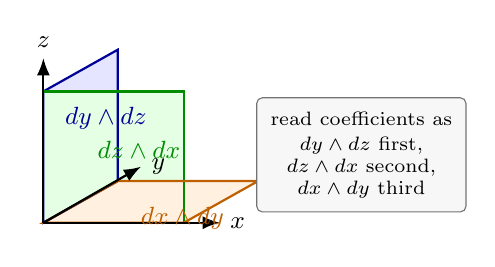
\begin{tikzpicture}[scale=1.15, every node/.style={font=\small}]
\coordinate (O) at (0,0);
\coordinate (X) at (1.55,0);
\coordinate (Y) at (0.82,0.46);
\coordinate (Z) at (0,1.45);
\fill[blue!10] (O) -- (Y) -- ($(Y)+(Z)$) -- (Z) -- cycle;
\fill[green!10] (O) -- (Z) -- ($(Z)+(X)$) -- (X) -- cycle;
\fill[orange!12] (O) -- (X) -- ($(X)+(Y)$) -- (Y) -- cycle;
\draw[thick, blue!60!black] (O) -- (Y) -- ($(Y)+(Z)$) -- (Z) -- cycle;
\draw[thick, green!55!black] (O) -- (Z) -- ($(Z)+(X)$) -- (X) -- cycle;
\draw[thick, orange!75!black] (O) -- (X) -- ($(X)+(Y)$) -- (Y) -- cycle;
\draw[vector] (O) -- (1.95,0) node[right] {$x$};
\draw[vector] (O) -- (1.08,0.62) node[right] {$y$};
\draw[vector] (O) -- (0,1.82) node[above] {$z$};
\node[blue!60!black] at ($(Y)!0.5!(Z)+(0.28,0.2)$) {$dy\wedge dz$};
\node[green!55!black] at ($(X)!0.5!(Z)+(0.28,0.08)$) {$dz\wedge dx$};
\node[orange!75!black] at ($(X)!0.5!(Y)+(0.35,-0.18)$) {$dx\wedge dy$};
\node[visualnode, anchor=west, font=\scriptsize] at (2.35,0.75)
{read coefficients as\\[1pt]
$dy\wedge dz$ first,\\
$dz\wedge dx$ second,\\
$dx\wedge dy$ third};
\end{tikzpicture}
\visualcaption{Each $2$-form basis element represents an oriented coordinate face. Reading those faces in cyclic order gives the vector-component order used for curl and flux.}
\end{center}

\subsection*{Problem 1(d): Divergence and $3$-forms}

\solutionflow{flux \(2\)-form\\\(\eta=F_1dy\,dz+\cdots\)}
{apply \(d\)\\only one term survives}
{coefficient of\\\(dx\,dy\,dz\) is \(\nabla\cdot F\)}
{Problem 1(d) is solved by noticing that repeated wedge factors vanish, leaving exactly the divergence coefficient.}

Throughout Problem 1(d) we work with a vector field $F=(F_1,F_2,F_3)$ and the associated flux $2$-form
\[
 \eta=F_1\,dy\wedge dz+F_2\,dz\wedge dx+F_3\,dx\wedge dy.
\]

\subsubsection*{Problem 1(d)-1: Compute $d\eta$}

Differentiate term by term:
\[
 d(F_1\,dy\wedge dz)=dF_1\wedge dy\wedge dz.
\]
Since
\[
 dF_1=(\pd_xF_1)\,dx+(\pd_yF_1)\,dy+(\pd_zF_1)\,dz,
\]
only the $dx$ term survives, because $dy\wedge dy=0$ and $dz\wedge dz=0$. Hence
\[
 d(F_1\,dy\wedge dz)=\pd_xF_1\,dx\wedge dy\wedge dz.
\]
The other two terms work the same way, after reordering the wedge products to $dx\wedge dy\wedge dz$. For completeness:
\[
\begin{aligned}
 d(F_2\,dz\wedge dx)
 &=dF_2\wedge dz\wedge dx\\
 &=(\pd_yF_2)\,dy\wedge dz\wedge dx\\
 &=(\pd_yF_2)\,dx\wedge dy\wedge dz,
\end{aligned}
\]
because $dy\wedge dz\wedge dx$ is a cyclic permutation of $dx\wedge dy\wedge dz$ and hence has positive sign. Also,
\[
\begin{aligned}
 d(F_3\,dx\wedge dy)
 &=dF_3\wedge dx\wedge dy\\
 &=(\pd_zF_3)\,dz\wedge dx\wedge dy\\
 &=(\pd_zF_3)\,dx\wedge dy\wedge dz.
\end{aligned}
\]
Adding all three surviving terms gives
\[
 d\eta
 =
 (\pd_xF_1+\pd_yF_2+\pd_zF_3)\,dx\wedge dy\wedge dz.
\]

\subsubsection*{Problem 1(d)-2: Compute $\nabla\cdot F$}

By definition,
\[
 \nabla\cdot F=\pd_xF_1+\pd_yF_2+\pd_zF_3.
\]

\subsubsection*{Problem 1(d)-3: The coefficient of $d\eta$ equals $\nabla\cdot F$}

Comparing the formula for $d\eta$ from 1(d)-1 with the formula for $\nabla\cdot F$ from 1(d)-2,
\[
 d\eta=(\nabla\cdot F)\,dx\wedge dy\wedge dz.
\]
That is, the single coefficient of the top-degree $3$-form $d\eta$ is exactly the divergence $\nabla\cdot F$.

\subsubsection*{Problem 1(d)-4: Correspondence between $\Omega^2(\R^3)$ and $\Omega^3(\R^3)$}

Under the identification
\[
 (A,B,C)\longleftrightarrow A\,dy\wedge dz+B\,dz\wedge dx+C\,dx\wedge dy
\]
between vector fields and $2$-forms, and the identification
\[
 \phi\longleftrightarrow \phi\,dx\wedge dy\wedge dz
\]
between functions and $3$-forms, the operation 1(d)-3 reads as
\[
 \eta\longmapsto d\eta\quad\Longleftrightarrow\quad F\longmapsto \nabla\cdot F.
\]
Hence
\[
 d:\Om^2(\R^3)\longrightarrow \Om^3(\R^3)
\]
is the differential-form version of divergence.

\subsection*{Problem 1(e): Summary}

\solutionflow{de Rham complex\\\(\Om^0\to\Om^1\to\Om^2\to\Om^3\)}
{vector calculus\\\(\nabla,\nabla\times,\nabla\cdot\)}
{\(d^2=0\)\\gives two identities}
{Problem 1(e) summarizes the whole dictionary and explains why curl-grad and div-curl vanish.}

With the coefficient identifications above, the de Rham complex
\[
 \Om^0(\R^3)
 \xrightarrow{d}
 \Om^1(\R^3)
 \xrightarrow{d}
 \Om^2(\R^3)
 \xrightarrow{d}
 \Om^3(\R^3)
\]
corresponds to the vector calculus sequence
\[
 \text{functions}
 \xrightarrow{\nabla}
 \text{vector fields}
 \xrightarrow{\nabla\times}
 \text{vector fields}
 \xrightarrow{\nabla\cdot}
 \text{functions}.
\]
The identity $d^2=0$ then contains the familiar identities
\[
 \nabla\times(\nabla f)=0,
 \qquad
 \nabla\cdot(\nabla\times F)=0.
\]
For example, starting from a function $f$, we have
\[
 f\xrightarrow{d}df\xrightarrow{d}d(df)=0.
\]
Under the vector calculus dictionary, this says
\[
 f\xrightarrow{\nabla}\nabla f\xrightarrow{\nabla\times}\nabla\times(\nabla f)=0.
\]
Likewise, starting from a vector field $F$ identified with a $1$-form $\omega$, the equality
\[
 d(d\omega)=0
\]
becomes
\[
 \nabla\cdot(\nabla\times F)=0.
\]

\section*{Problem 2: Computing the Winding $1$-Form on the Unit Circle}

\begin{intentrequirements}
\item \textbf{Intent.} Show that the winding $1$-form
\[
 \omega=\frac{-y\,dx+x\,dy}{x^2+y^2}
\]
measures angular change around the origin, and verify that one positive trip around the unit circle contributes total angle $2\pi$.
\item \textbf{Required outputs.} Compute the integral over $S^1$ by three methods: the angular parameterization $x=\cos\theta$, $y=\sin\theta$; the semicircle method using $x^2+y^2=1$; and the complex-variable identity $\omega=\operatorname{Im}(dz/z)$.
\item \textbf{Required explanations.} Explain the orientation in every method. In the semicircle method, the upper semicircle runs from $x=1$ to $x=-1$, while the lower semicircle runs from $x=-1$ to $x=1$. The solution must say why both contributions are positive.
\item \textbf{Common pitfalls to avoid.} Do not divide by $y$ globally on the whole circle. The points where $y=0$ force the split into upper and lower semicircles.
\end{intentrequirements}

The winding form on $\R^2\setminus\{0\}$ is
\[
 \omega=\frac{-y\,dx+x\,dy}{x^2+y^2}.
\]
On the unit circle $S^1$, we have $x^2+y^2=1$, so along $S^1$ this becomes
\[
 \omega|_{S^1}=-y\,dx+x\,dy.
\]
We use the positive, counterclockwise orientation.
Geometrically, $\omega$ measures infinitesimal change of angle. Therefore the final answer should be the total change of angle during one counterclockwise trip around the circle, namely $2\pi$. The computations below verify this in three different coordinate languages.

\windingnote{Three properties of $\omega$ are decisive for this entire exam.
\emph{(i)~Closedness.} The coefficient functions $P=\tfrac{-y}{x^2+y^2}$ and $Q=\tfrac{x}{x^2+y^2}$ satisfy $\partial_yP=\partial_xQ=\tfrac{y^2-x^2}{(x^2+y^2)^2}$, so $d\omega=(\partial_xQ-\partial_yP)\,dx\wedge dy=0$.
\emph{(ii)~Non-exactness on $\R^2\setminus\{0\}$.} If $\omega$ were $d\eta$ for some smooth function $\eta$, then by Stokes $\oint_{S^1}\omega=0$; but the computations below give $2\pi$, so no such global $\eta$ exists. Locally, on any simply-connected open set avoiding the origin, $\omega=d(\arg(x+iy))$ is exact; the obstruction is purely topological --- a wound in the domain.
\emph{(iii)~Complex avatar.} Writing $z=x+iy$, the identity $\omega=\operatorname{Im}(dz/z)$ from part~(c) shows the winding form is the imaginary part of the holomorphic logarithmic differential. Hence $\oint_{S^1}\omega=\operatorname{Im}\bigl(\oint_{S^1}dz/z\bigr)=\operatorname{Im}(2\pi i)=2\pi$. The same $2\pi i$ powers the Cauchy integral formula (Problem~3) and the residue theorem on Riemann surfaces (final Problems~8 and~9).}

\handsketch{%
\fill[handpaper] (-3.4,-1.9) rectangle (3.4,1.9);
\draw[hand] (-3.4,-1.9) rectangle (3.4,1.9);
% Circle (using a polygon approximation for handdrawn feel)
\draw[handthick] (0,0) circle (1.45);
\draw[draw=handink, dashed, line width=0.3pt, opacity=0.6] (-1.7,0) -- (1.7,0);
\draw[draw=handink, dashed, line width=0.3pt, opacity=0.6] (0,-1.7) -- (0,1.7);
% Radial spoke
\draw[draw=handink, line width=0.5pt] (0,0) -- (40:1.45);
\node[handnote, anchor=south west] at (40:1.55) {$z=e^{i\theta}$};
% Angle arc (plain, no decoration)
\draw[draw=handink, line width=0.5pt, -{Latex[length=1.6mm]}] (12:0.45) arc (12:38:0.45);
\node[handnote] at (28:0.7) {$\theta$};
% Tangent: dz/z direction
\draw[draw=handink, line width=0.7pt, -{Latex[length=1.8mm]}] (40:1.45) -- ++(130:0.55);
\coordinate (DTHL) at ($(40:1.45)+(130:0.7)$);
\node[handnote] at (DTHL) {$d\theta$};
% Counterclockwise full loop arrow (plain arc)
\draw[draw=handink, line width=0.6pt, -{Latex[length=1.8mm]}] (110:1.45) arc (110:175:1.45);
% Labels
\node[handnote] at (2.3,1.5) {$\omega|_{S^1}=d\theta$};
\node[handnote] at (2.3,1.05) {$\oint_{S^1}\omega=2\pi$};
\node[handnote] at (-2.45,-1.5) {$\omega=\mathrm{Im}\,\dfrac{dz}{z}$};
}

\begin{center}
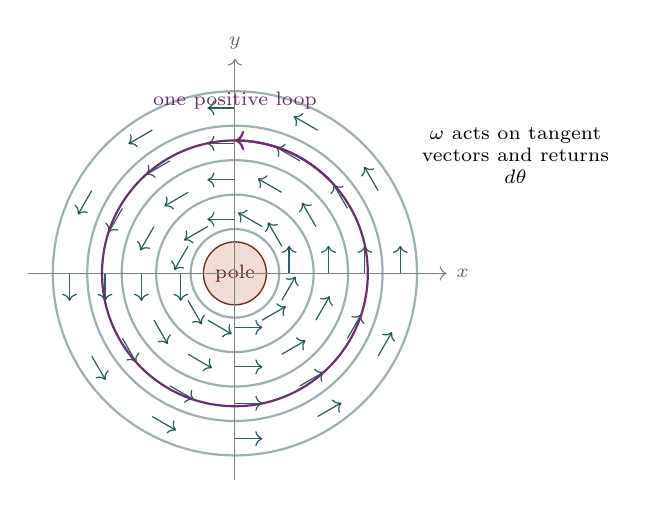
\begin{tikzpicture}[scale=1.25, every node/.style={font=\scriptsize}]
% Background: angular field around origin
\foreach \r in {0.45,0.8,1.15,1.5,1.85}{
  \draw[geodesic, formteal!50!black, opacity=0.4] (0,0) circle (\r);
}
\foreach \th in {0,30,...,330}{
  \pgfmathsetmacro\rstart{0.35}
  \pgfmathsetmacro\rend{1.85}
  \foreach \rr in {0.55,0.95,1.32,1.68}{
    \draw[->, formteal!60!black, line width=0.45pt, opacity=0.85]
      (\th:\rr) -- ++({\th+90}:0.28);
  }
}
% Origin singularity
\fill[white] (0,0) circle (0.32);
\draw[draw=formrust!70!black, fill=formrust!18, line width=0.5pt] (0,0) circle (0.32);
\node[formrust!60!black, font=\scriptsize] at (0,0) {pole};
% Axes
\draw[->, black!50, line width=0.4pt] (-2.1,0) -- (2.15,0) node[right, black!60] {$x$};
\draw[->, black!50, line width=0.4pt] (0,-2.1) -- (0,2.18) node[above, black!60] {$y$};
% Sample integration curve (closed loop)
\draw[formplum, line width=0.8pt] (1.35,0) arc (0:360:1.35);
\draw[->, formplum, line width=0.8pt] (45:1.35) arc (45:90:1.35);
\node[formplum, font=\scriptsize] at (0,1.75) {one positive loop};
% Caption inside
\node[font=\scriptsize, align=center] at (2.85,1.2) {$\omega$ acts on tangent\\vectors and returns\\$d\theta$};
\end{tikzpicture}
\visualcaption{The winding form is a rotational covector field on $\R^2\setminus\{0\}$. Along any positively oriented loop encircling the puncture, $\omega$ accumulates the total angular increment $2\pi n$ where $n$ is the winding number.}
\end{center}

\begin{center}
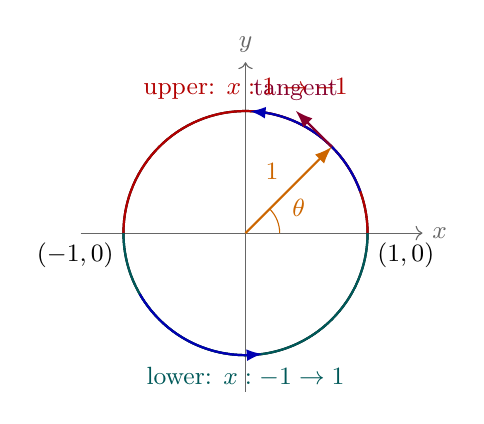
\begin{tikzpicture}[scale=1.55, every node/.style={font=\small}]
\draw[->, black!60] (-1.35,0) -- (1.45,0) node[right] {$x$};
\draw[->, black!60] (0,-1.3) -- (0,1.4) node[above] {$y$};
\draw[thick] (0,0) circle (1);
\draw[thick, red!70!black] (1,0) arc (0:180:1);
\draw[thick, teal!70!black] (-1,0) arc (180:360:1);
\draw[formarrow, blue!70!black] (20:1) arc (20:88:1);
\draw[formarrow, blue!70!black] (210:1) arc (210:278:1);
\draw[vector, orange!80!black] (0,0) -- (45:1) node[midway, above left] {$1$};
\draw[vector, purple!70!black] (45:1) -- ++(135:0.42) node[above] {tangent};
\draw[thin, orange!80!black] (0.28,0) arc (0:45:0.28);
\node[orange!80!black] at (25:0.48) {$\theta$};
\node[red!70!black] at (0,1.18) {upper: $x:1\to -1$};
\node[teal!70!black] at (0,-1.18) {lower: $x:-1\to 1$};
\node[below right] at (1,0) {$(1,0)$};
\node[below left] at (-1,0) {$(-1,0)$};
\end{tikzpicture}
\visualcaption{The winding form measures the angular change $d\theta$. The semicircle split records why the two $x$-coordinate integrals have opposite limits but both contribute positively.}
\end{center}

\subsection*{Problem 2(a): Angular parameterization}

\solutionflow{\(x=\cos\theta\)\\\(y=\sin\theta\)}
{pull back\\\(-y\,dx+x\,dy\)}
{\(\gamma^*\omega=d\theta\)\\integral \(=2\pi\)}
{Problem 2(a) is solved by choosing the global angular parameter and pulling the form back to \(d\theta\).}

Parametrize the unit circle by
\[
 x=\cos\theta,\qquad y=\sin\theta,\qquad 0\leq \theta\leq 2\pi.
\]
This parameterization is counterclockwise: at $\theta=0$ the point is $(1,0)$ and the velocity is $(0,1)$, pointing upward.
Then
\[
 dx=-\sin\theta\,d\theta,\qquad dy=\cos\theta\,d\theta.
\]
Substitute into the form:
\[
\begin{aligned}
 -y\,dx+x\,dy
 &=-\sin\theta(-\sin\theta\,d\theta)
   +\cos\theta(\cos\theta\,d\theta)\\
 &=(\sin^2\theta+\cos^2\theta)\,d\theta\\
 &=d\theta.
\end{aligned}
\]
In pullback notation, what we have shown is
\[
 \gamma^*\omega=d\theta,
\]
where $\gamma(\theta)=(\cos\theta,\sin\theta)$. Therefore the integral over the curve becomes an ordinary one-variable integral:
\[
 \int_{S^1}\omega=\int_{[0,2\pi]}\gamma^*\omega.
\]
Therefore
\[
 \int_{S^1}\omega=\int_0^{2\pi}d\theta=2\pi.
\]
This also explains why the winding form has its name: the integral records one full winding around the origin.

\subsection*{Problem 2(b): Using the relation $x^2+y^2=1$}

\solutionflow{constraint\\\(x^2+y^2=1\)}
{differentiate\\\(x\,dx+y\,dy=0\)}
{split circle\\upper \(+\) lower}
{Problem 2(b) is solved by using \(x\) as a local coordinate separately on the two semicircles.}

On $S^1$,
\[
 x^2+y^2=1.
\]
Differentiating along the circle gives
\[
 2x\,dx+2y\,dy=0,
 \qquad\text{so}\qquad
 x\,dx+y\,dy=0.
\]
To use this safely, split the circle into the upper and lower semicircles.
We split because solving for $dy$ in terms of $dx$ requires dividing by $y$, and $y=0$ at the two endpoints $(1,0)$ and $(-1,0)$. The endpoints do not affect the integral, but the upper and lower semicircles have different signs for $y$.

On the upper semicircle, $y=\sqrt{1-x^2}$ and the counterclockwise orientation runs from $x=1$ to $x=-1$. Since
\[
 dy=-\frac{x}{y}\,dx,
\]
we get
\[
\begin{aligned}
 \omega
 &=-y\,dx+x\,dy\\
 &=-y\,dx+x\left(-\frac{x}{y}\,dx\right)\\
 &=-\frac{x^2+y^2}{y}\,dx\\
 &=-\frac{1}{y}\,dx.
\end{aligned}
\]
Thus
\[
 \int_{\text{upper}}\omega
 =
 \int_1^{-1}-\frac{dx}{\sqrt{1-x^2}}
 =
 \int_{-1}^{1}\frac{dx}{\sqrt{1-x^2}}
 =\pi.
\]
The last equality comes from
\[
 \int\frac{dx}{\sqrt{1-x^2}}=\arcsin x,
\]
so
\[
 \int_{-1}^{1}\frac{dx}{\sqrt{1-x^2}}
 =
 \arcsin(1)-\arcsin(-1)
 =
 \frac{\pi}{2}-\left(-\frac{\pi}{2}\right)=\pi.
\]

On the lower semicircle, $y=-\sqrt{1-x^2}$ and the counterclockwise orientation runs from $x=-1$ to $x=1$. The same simplification gives
\[
 \omega=-\frac{1}{y}\,dx
 =
 \frac{dx}{\sqrt{1-x^2}}.
\]
Hence
\[
 \int_{\text{lower}}\omega
 =
 \int_{-1}^{1}\frac{dx}{\sqrt{1-x^2}}
 =\pi.
\]
Notice that both semicircle integrals are positive. The sign from $y<0$ on the lower semicircle is exactly compensated by the orientation running from $x=-1$ to $x=1$.
Adding the two semicircles,
\[
 \int_{S^1}\omega=\pi+\pi=2\pi.
\]
This method is longer than the angular parameterization because $x$ is not a single-valued coordinate on the whole circle. Splitting into two pieces is the price of using $x$ as a local coordinate.

\subsection*{Problem 2(c): Complex-variable method}

\solutionflow{write\\\(z=x+iy\)}
{split\\\(\dfrac{dz}{z}\) into real and imaginary parts}
{\(\operatorname{Im}(dz/z)=\omega\)\\so integral \(=2\pi\)}
{Problem 2(c) is solved by recognizing the winding form as the angular part of \(dz/z\).}

Let
\[
 z=x+iy,\qquad dz=dx+i\,dy.
\]
The reciprocal of $z$ is
\[
 \frac1z=\frac{\bar z}{|z|^2}=\frac{x-iy}{x^2+y^2}.
\]
Then
\[
\begin{aligned}
 \frac{dz}{z}
 &=
 \frac{dx+i\,dy}{x+iy}\\
 &=
 \frac{(dx+i\,dy)(x-iy)}{x^2+y^2}\\
 &=
 \frac{x\,dx+y\,dy}{x^2+y^2}
 +i\,\frac{x\,dy-y\,dx}{x^2+y^2}.
\end{aligned}
\]
Therefore
\[
 \omega
 =
 \frac{-y\,dx+x\,dy}{x^2+y^2}
 =
 \operatorname{Im}\left(\frac{dz}{z}\right).
\]
The real part of $dz/z$ is
\[
 \frac{x\,dx+y\,dy}{x^2+y^2},
\]
which measures radial change. On the unit circle the radius is constant, so the radial part vanishes along tangent directions. The imaginary part is the angular part, which is why it equals the winding form.

\begin{center}
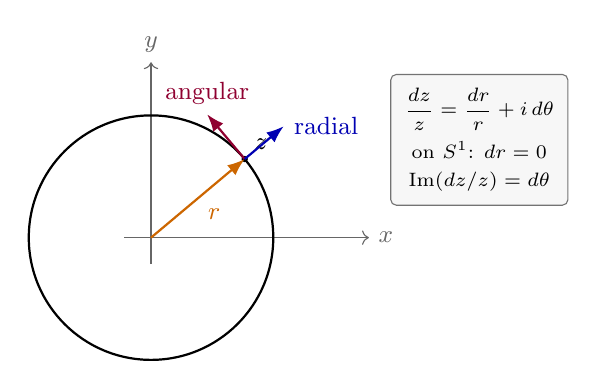
\begin{tikzpicture}[scale=1.35, every node/.style={font=\small}]
\draw[->, black!60] (-0.25,0) -- (2.05,0) node[right] {$x$};
\draw[->, black!60] (0,-0.25) -- (0,1.65) node[above] {$y$};
\draw[thick] (0,0) circle (1.15);
\coordinate (P) at (40:1.15);
\fill (P) circle (0.03) node[above right] {$z$};
\draw[vector, orange!80!black] (0,0) -- (P) node[midway, below right] {$r$};
\draw[vector, purple!75!black] (P) -- ++(130:0.55) node[above] {angular};
\draw[vector, blue!70!black] (P) -- ++(40:0.48) node[right] {radial};
\node[visualnode, anchor=west, font=\scriptsize] at (2.25,0.92)
{$\displaystyle \frac{dz}{z}=\frac{dr}{r}+i\,d\theta$\\[3pt]
on $S^1$: $dr=0$\\[2pt]
$\operatorname{Im}(dz/z)=d\theta$};
\end{tikzpicture}
\visualcaption{The complex calculation separates motion into radial and angular pieces. The unit circle kills the radial term, leaving exactly the winding form.}
\end{center}
On the unit circle, $z=e^{i\theta}$, so
\[
 dz=i e^{i\theta}\,d\theta,
 \qquad
 \frac{dz}{z}=i\,d\theta.
\]
Taking imaginary parts gives
\[
 \omega=d\theta.
\]
Thus
\[
 \int_{S^1}\omega=2\pi.
\]
Equivalently,
\[
 \int_{S^1}\frac{dz}{z}=2\pi i,
 \qquad
 \int_{S^1}\omega=\operatorname{Im}(2\pi i)=2\pi.
\]

\section*{Problem 3: Cauchy--Green Formula via the Generalized Stokes Theorem}

\begin{intentrequirements}
\item \textbf{Intent.} Derive the Cauchy--Green formula by applying the generalized Stokes theorem to a punctured domain, where the puncture removes the pole of
\[
 \alpha(\omega)=\frac{f(\omega)}{\omega-z}\,d\omega.
\]
\item \textbf{Required outputs.} Identify the boundary of $\Omega_\eps$, compute $d\alpha$, compute the $\bar\omega$-derivative of $f(\omega)/(\omega-z)$, apply Stokes' theorem, evaluate the small-circle limit, and pass to the limit $\eps\to0$.
\item \textbf{Required explanations.} Track the three sign sources separately: the inner boundary orientation, the order of $d\omega\wedge d\bar\omega$ versus $d\bar\omega\wedge d\omega$, and the positive orientation in the small-circle integral.
\item \textbf{Analytic requirement.} Justify why the punctured-domain integral converges as the disk radius shrinks. The singularity behaves like $1/|\omega-z|$, which is integrable in two real dimensions because the area element contributes a factor $r\,dr\,d\theta$.
\end{intentrequirements}

Let $\Omega\subset\C$ be bounded with smooth boundary, let $f\in C^1(\Omega)$, and fix $z\in\Omega$. For small $\eps>0$, define
\[
 \Omega_\eps=\Omega\setminus B_\eps(z),
 \qquad
 \alpha(\omega)=\frac{f(\omega)}{\omega-z}\,d\omega.
\]
It is convenient to set
\[
 g(\omega)=\frac{f(\omega)}{\omega-z},
 \qquad
 \alpha=g\,d\omega.
\]
The reason for deleting the small disk is that $\alpha$ has a pole at $\omega=z$. On $\Omega_\eps$ the form is smooth, so Stokes' theorem can be applied without ambiguity.

\windingnote{The puncture-and-Stokes machinery here is the direct generalization of the winding-form integral of Problem~2. After translating $\omega\mapsto\omega-z$, the form $d\omega/(\omega-z)$ \emph{is} (the holomorphic avatar of) the winding form centered at $z$: parametrizing the small circle by $\omega=z+\eps e^{it}$ gives $d\omega/(\omega-z)=i\,dt$, whose imaginary part is exactly the angular form $dt$. The factor $2\pi i$ that emerges as the small-circle limit in part~(e) is the same $2\pi$ from $\oint_{S^1}\omega_{\text{wind}}=2\pi$, dressed up with the imaginary unit because we are now integrating the full complex form $dz/(\omega-z)$ rather than just its imaginary part. The Cauchy integral formula is, in this sense, ``the winding integral with a function $f$ riding on top''.}

\handsketch{%
\fill[handpaper] (-3.4,-1.95) rectangle (3.4,1.95);
\draw[hand] (-3.4,-1.95) rectangle (3.4,1.95);
% Domain shape (Omega)
\draw[handthick] plot[smooth cycle] coordinates {(-2.4,-1.05) (-2.0,0.85) (-0.65,1.3) (1.05,0.95) (2.05,0.5) (2.45,-0.7) (1.25,-1.45) (-0.7,-1.3)};
\node[handnote] at (-2.0,1.45) {$\Omega$};
% z point
\fill[handink] (0.45,0.05) circle (0.06);
\node[handnote] at (0.45,-0.25) {$z$};
% Small disks (shrinking)
\draw[draw=handink, line width=0.4pt, opacity=0.8] (0.45,0.05) circle (0.92);
\draw[draw=handink, line width=0.4pt, opacity=0.8] (0.45,0.05) circle (0.58);
\draw[draw=handink, line width=0.85pt] (0.45,0.05) circle (0.28);
\draw[draw=handink, line width=0.55pt, -{Latex[length=1.7mm]}] ($(0.45,0.05)+(40:0.28)$) arc (40:160:0.28);
\node[handnote] at (1.45,0.5) {$\varepsilon\to 0$};
% Result on the right
\node[handnote] at (2.4,1.5) {$\displaystyle\oint_{\partial B_\varepsilon(z)}\!\!\dfrac{f(\omega)}{\omega-z}d\omega$};
\node[handnote] at (2.4,1.05) {$\longrightarrow 2\pi i\,f(z)$};
\node[handnote] at (-2.1,-1.45) {$=\!2\pi i\cdot$ winding};
}

\begin{center}
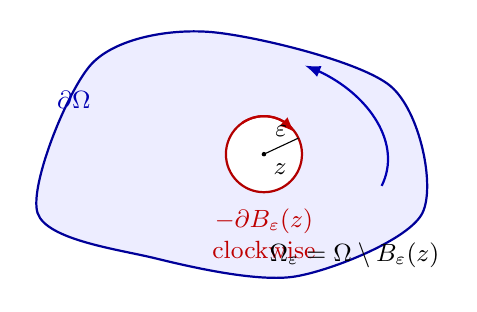
\begin{tikzpicture}[scale=1.15, every node/.style={font=\small}]
\coordinate (z0) at (0.35,0.1);
\filldraw[region]
  plot[smooth cycle] coordinates {(-2.15,-0.55) (-1.55,1.1) (-0.25,1.45) (1.75,0.85) (2.1,-0.55) (0.7,-1.25) (-0.85,-1.05)};
\filldraw[hole] (z0) circle (0.42);
\draw[formarrow, blue!70!black] (1.65,-0.25) .. controls (1.9,0.25) and (1.45,0.85) .. (0.8,1.08);
\draw[formarrow, red!75!black] ($(z0)+(125:0.42)$) arc (125:35:0.42);
\fill[black] (z0) circle (0.025) node[below right] {$z$};
\draw[thin] (z0) -- ++(25:0.42) node[midway, above] {$\eps$};
\node[blue!70!black] at (-1.75,0.7) {$\partial\Omega$};
\node[red!75!black, align=center] at (0.35,-0.78) {$-\partial B_\eps(z)$\\clockwise};
\node at (1.35,-1.02) {$\Omega_\eps=\Omega\setminus B_\eps(z)$};
\end{tikzpicture}
\visualcaption{The puncture removes the pole. The outer boundary remains counterclockwise, while the induced boundary orientation around the hole is clockwise.}
\end{center}

\subsection*{Problem 3(a): Boundary of the punctured domain}

\solutionflow{delete disk\\\(B_\eps(z)\)}
{boundary has\\outer plus inner}
{inner orientation\\is negative}
{Problem 3(a) is solved by applying the region-on-left orientation rule to the punctured domain.}

The boundary of $\Omega_\eps$ has two pieces. The outer boundary keeps the positive orientation of $\partial\Omega$. The inner circle is a hole, so its induced orientation is the opposite of the usual positive orientation around the disk. Therefore
\[
 \partial\Omega_\eps=\partial\Omega\cup(-\partial B_\eps(z)).
\]
Hence
\[
 \int_{\partial\Omega_\eps}\alpha
 =
 \int_{\partial\Omega}\frac{f(\omega)}{\omega-z}\,d\omega
 -
 \int_{\partial B_\eps(z)}\frac{f(\omega)}{\omega-z}\,d\omega.
\]
One way to remember the minus sign is this: if you walk along the positively oriented boundary of a region, the region stays on your left. Around the inner circle, the punctured region lies outside the small disk, so the induced orientation is clockwise. The usual positive orientation of $\partial B_\eps(z)$ is counterclockwise, hence the minus sign.

\subsection*{Problem 3(b): Exterior derivative of the $1$-form}

\solutionflow{\(\alpha=g\,d\omega\)}
{compute\\\(d\alpha=dg\wedge d\omega\)}
{only\\\(\pd_{\bar\omega}g\,d\bar\omega\wedge d\omega\)}
{Problem 3(b) is solved by expanding \(dg\) in Wirtinger coordinates and using \(d\omega\wedge d\omega=0\).}

Since $\alpha=g\,d\omega$,
\[
 d\alpha=d(g\,d\omega)=dg\wedge d\omega+g\,d(d\omega).
\]
Because $d(d\omega)=0$, this reduces to
\[
 d\alpha=dg\wedge d\omega.
\]
In Wirtinger notation,
\[
 dg=\frac{\pd g}{\pd\omega}\,d\omega
 +\frac{\pd g}{\pd\bar\omega}\,d\bar\omega.
\]
Here $d\omega$ and $d\bar\omega$ play the role of the coordinate $1$-forms for the complex coordinates $\omega,\bar\omega$. The key wedge-product rules are
\[
 d\omega\wedge d\omega=0,\qquad
 d\bar\omega\wedge d\bar\omega=0,\qquad
 d\bar\omega\wedge d\omega=-d\omega\wedge d\bar\omega.
\]
If $\omega=\xi+i\eta$, then
\[
 d\omega=d\xi+i\,d\eta,\qquad d\bar\omega=d\xi-i\,d\eta.
\]
Consequently,
\[
 d\omega\wedge d\bar\omega
 =
 (d\xi+i\,d\eta)\wedge(d\xi-i\,d\eta)
 =
 -2i\,d\xi\wedge d\eta.
\]
So $d\omega\wedge d\bar\omega$ is, up to the constant $-2i$, the usual oriented area form in the $\omega$-plane.
Thus
\[
\begin{aligned}
 d\alpha
 &=
 \left(
 \frac{\pd g}{\pd\omega}\,d\omega
 +\frac{\pd g}{\pd\bar\omega}\,d\bar\omega
 \right)\wedge d\omega\\
 &=
 \frac{\pd g}{\pd\omega}\,d\omega\wedge d\omega
 +
 \frac{\pd g}{\pd\bar\omega}\,d\bar\omega\wedge d\omega.
\end{aligned}
\]
The first term is zero because $d\omega\wedge d\omega=0$. Therefore
\[
 d\alpha=
 \frac{\pd g}{\pd\bar\omega}\,d\bar\omega\wedge d\omega.
\]
Equivalently,
\[
 d\alpha=
 -\frac{\pd g}{\pd\bar\omega}\,d\omega\wedge d\bar\omega.
\]
The $\bar\omega$-derivative is the derivative that survives because it is paired with $d\bar\omega\wedge d\omega$. The $\omega$-derivative is multiplied by $d\omega\wedge d\omega$, which is zero.

\subsection*{Problem 3(c): Computing the derivative}

\solutionflow{\(g=f(\omega)(\omega-z)^{-1}\)}
{product rule\\in \(\bar\omega\)}
{holomorphic factor\\has zero \(\bar\omega\)-derivative}
{Problem 3(c) is solved by observing that the pole factor is holomorphic away from the deleted point.}

We have
\[
 g(\omega)=f(\omega)\frac{1}{\omega-z}.
\]
On $\Omega_\eps$, the function $(\omega-z)^{-1}$ is holomorphic in $\omega$, so
\[
 \frac{\pd}{\pd\bar\omega}\left(\frac{1}{\omega-z}\right)=0.
\]
Therefore
\[
 \frac{\pd g}{\pd\bar\omega}
 =
 \frac{1}{\omega-z}\frac{\pd f}{\pd\bar\omega}.
\]
This is just the product rule:
\[
 \pd_{\bar\omega}\left(f(\omega)(\omega-z)^{-1}\right)
 =
 (\pd_{\bar\omega}f)(\omega-z)^{-1}
 +
 f\,\pd_{\bar\omega}\left((\omega-z)^{-1}\right),
\]
and the second term is zero.
Substituting into the previous part gives
\[
 d\alpha
 =
 \frac{\pd f/\pd\bar\omega}{\omega-z}\,
 d\bar\omega\wedge d\omega
 =
 -\frac{\pd f/\pd\bar\omega}{\omega-z}\,
 d\omega\wedge d\bar\omega.
\]

\begin{center}
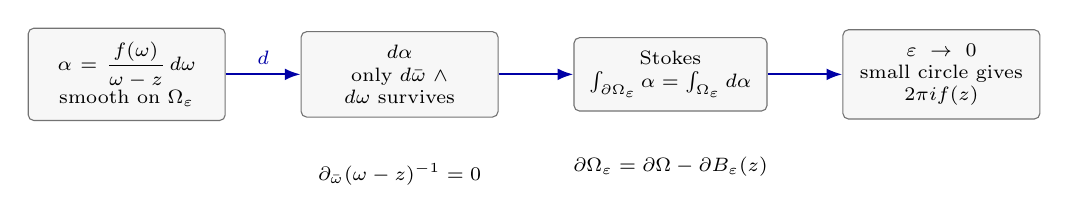
\begin{tikzpicture}[node distance=0.95cm, every node/.style={font=\scriptsize}]
\node[visualnode, text width=2.15cm] (a) {$\alpha=\dfrac{f(\omega)}{\omega-z}\,d\omega$\\smooth on $\Omega_\eps$};
\node[visualnode, text width=2.15cm, right=of a] (d) {$d\alpha$\\only $d\bar\omega\wedge d\omega$ survives};
\node[visualnode, text width=2.1cm, right=of d] (stokes) {Stokes\\$\int_{\partial\Omega_\eps}\alpha=\int_{\Omega_\eps}d\alpha$};
\node[visualnode, text width=2.15cm, right=of stokes] (limit) {$\eps\to0$\\small circle gives\\$2\pi i f(z)$};
\draw[formarrow] (a) -- node[above] {$d$} (d);
\draw[formarrow] (d) -- (stokes);
\draw[formarrow] (stokes) -- (limit);
\node[below=0.45cm of d, align=center, font=\scriptsize] {$\partial_{\bar\omega}(\omega-z)^{-1}=0$};
\node[below=0.45cm of stokes, align=center, font=\scriptsize] {$\partial\Omega_\eps=\partial\Omega-\partial B_\eps(z)$};
\end{tikzpicture}
\visualcaption{The Cauchy--Green computation is a four-step pipeline: remove the pole, differentiate the smooth form, apply Stokes, then shrink the deleted circle.}
\end{center}

\subsection*{Problem 3(d): Apply the generalized Stokes theorem}

\solutionflow{smooth form\\on \(\Omega_\eps\)}
{Stokes\\\(\int_{\partial\Omega_\eps}\alpha=\int_{\Omega_\eps}d\alpha\)}
{substitute\\boundary and \(d\alpha\)}
{Problem 3(d) is solved by combining the boundary decomposition with the exterior derivative computed in the previous parts.}

The generalized Stokes theorem says
\[
 \int_{\partial\Omega_\eps}\alpha
 =
 \iint_{\Omega_\eps}d\alpha.
\]
The hypotheses needed here are satisfied because $\Omega_\eps$ is a compact region with smooth boundary pieces and $\alpha$ is smooth on $\Omega_\eps$. The original pole at $\omega=z$ has been removed.
Using parts (a)--(c),
\[
 \int_{\partial\Omega}\frac{f(\omega)}{\omega-z}\,d\omega
 -
 \int_{\partial B_\eps(z)}\frac{f(\omega)}{\omega-z}\,d\omega
 =
 \iint_{\Omega_\eps}
 \frac{\pd f/\pd\bar\omega}{\omega-z}\,
 d\bar\omega\wedge d\omega.
\]
If we prefer to write the area form in the order $d\omega\wedge d\bar\omega$, then this is
\[
 \int_{\partial\Omega}\frac{f(\omega)}{\omega-z}\,d\omega
 -
 \int_{\partial B_\eps(z)}\frac{f(\omega)}{\omega-z}\,d\omega
 =
 -
 \iint_{\Omega_\eps}
 \frac{\pd f/\pd\bar\omega}{\omega-z}\,
 d\omega\wedge d\bar\omega.
\]

\subsection*{Problem 3(e): Limit of the small circle integral}

\solutionflow{parametrize\\\(\omega=z+\eps e^{it}\)}
{cancel\\\(\eps e^{it}\)}
{continuity gives\\\(2\pi i f(z)\)}
{Problem 3(e) is solved by reducing the small-circle integral to an average of \(f\) over a shrinking circle.}

Parametrize the positively oriented small circle by
\[
 \omega=z+\eps e^{it},\qquad 0\leq t\leq 2\pi.
\]
This is the counterclockwise orientation of the circle $\partial B_\eps(z)$. Recall that in $\partial\Omega_\eps$ this circle appears with the opposite orientation, but in part (e) the integral is over $\partial B_\eps(z)$ itself, so we use the positive counterclockwise parameterization.
Then
\[
 d\omega=i\eps e^{it}\,dt,
 \qquad
 \omega-z=\eps e^{it}.
\]
Therefore
\[
\begin{aligned}
 \int_{\partial B_\eps(z)}
 \frac{f(\omega)}{\omega-z}\,d\omega
 &=
 \int_0^{2\pi}
 \frac{f(z+\eps e^{it})}{\eps e^{it}}
 i\eps e^{it}\,dt\\
 &=
 i\int_0^{2\pi}f(z+\eps e^{it})\,dt.
\end{aligned}
\]
Since $f$ is continuous,
\[
 f(z+\eps e^{it})\longrightarrow f(z)
\]
uniformly in $t$ as $\eps\to0$. Hence
\[
 \lim_{\eps\to0}
 \int_{\partial B_\eps(z)}
 \frac{f(\omega)}{\omega-z}\,d\omega
 =
 i\int_0^{2\pi}f(z)\,dt
 =
 2\pi i\,f(z).
\]

\begin{center}
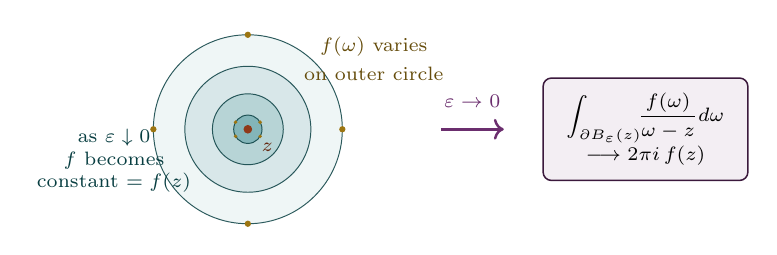
\begin{tikzpicture}[scale=1.0, every node/.style={font=\scriptsize}]
% Three nested circles representing shrinking
\foreach \rr/\op/\xx in {1.2/8/0, 0.8/18/0, 0.45/32/0, 0.18/55/0}{
  \filldraw[draw=formteal!55!black, fill=formteal!\op, line width=0.35pt, opacity=0.85]
    (\xx,0) circle (\rr);
}
% Center: the point z
\fill[formrust!85!black] (0,0) circle (0.055);
\node[formrust!60!black, font=\scriptsize, below right] at (0.05,-0.05) {$z$};
% Sample f-values on the outermost circle (showing variation)
\foreach \th/\fv in {0/{f(z{+}\eps)}, 90/{f}, 180/{f}, 270/{f}}{
  \fill[formgold!85!black] (\th:1.2) circle (0.04);
}
\node[formgold!55!black, font=\scriptsize] at (1.6,1.05) {$f(\omega)$ varies};
\node[formgold!55!black, font=\scriptsize] at (1.6,0.7) {on outer circle};
% Inner circle: f essentially constant ≈ f(z)
\foreach \th in {30,150,210,330}{
  \fill[formgold!85!black] (\th:0.18) circle (0.025);
}
\node[formteal!55!black, font=\scriptsize, align=center] at (-1.7,-0.4) {as $\eps\downarrow 0$\\$f$ becomes\\constant $=f(z)$};
% Arrow showing limit
\draw[->, formplum, line width=0.9pt] (2.45,0) -- (3.25,0);
\node[formplum, font=\scriptsize] at (2.85,0.35) {$\eps\to 0$};
% Right: limit value 2pi i f(z)
\node[draw=formplum!55!black, fill=formplum!8, rounded corners=3pt, line width=0.55pt,
      align=center, minimum width=2.6cm, minimum height=1.3cm] at (5.05,0)
      {$\displaystyle\int_{\partial B_\eps(z)}\!\!\frac{f(\omega)}{\omega-z}d\omega$\\$\longrightarrow 2\pi i\,f(z)$};
\end{tikzpicture}
\visualcaption{Shrinking the contour replaces $f$ by its value at the center: each loop contributes the average of $f$ over the circle, and continuity drives that average to $f(z)$. The factor $2\pi i$ comes from $d\omega/(\omega-z)$ on the parametrized circle.}
\end{center}

\subsection*{Problem 3(f): Cauchy--Green formula}

\solutionflow{rearrange\\Stokes identity}
{let\\\(\eps\to0\)}
{divide by\\\(2\pi i\)}
{Problem 3(f) is solved by moving the small-circle term to one side and passing to the limit.}

From part (d), using the $d\omega\wedge d\bar\omega$ order,
\[
 \int_{\partial\Omega}\frac{f(\omega)}{\omega-z}\,d\omega
 -
 \int_{\partial B_\eps(z)}\frac{f(\omega)}{\omega-z}\,d\omega
 =
 -
 \iint_{\Omega_\eps}
 \frac{\pd f/\pd\bar\omega}{\omega-z}\,
 d\omega\wedge d\bar\omega.
\]
Rearranging,
\[
 \int_{\partial B_\eps(z)}\frac{f(\omega)}{\omega-z}\,d\omega
 =
 \int_{\partial\Omega}\frac{f(\omega)}{\omega-z}\,d\omega
 +
 \iint_{\Omega_\eps}
 \frac{\pd f/\pd\bar\omega}{\omega-z}\,
 d\omega\wedge d\bar\omega.
\]
Now let $\eps\to0$. The small circle integral tends to $2\pi i f(z)$, and the punctured-domain integral tends to the integral over $\Omega$ because the singularity is integrable. Thus
\[
 \int_{\{\eps<|\omega-z|<\eps_0\}}
 \left|\frac{\pd f/\pd\bar\omega}{\omega-z}\right|\,dA
 \leq
 C\int_\eps^{\eps_0}\int_0^{2\pi}\frac{1}{r}r\,d\theta\,dr,
\]
so the singularity is mild enough for the limit. In particular, the contribution of the deleted disk tends to zero as its radius tends to zero.
\[
 2\pi i f(z)
 =
 \int_{\partial\Omega}\frac{f(\omega)}{\omega-z}\,d\omega
 +
 \iint_{\Omega}
 \frac{\pd f/\pd\bar\omega}{\omega-z}\,
 d\omega\wedge d\bar\omega.
\]
Therefore
\[
 \boxed{
 f(z)=
 \frac{1}{2\pi i}
 \int_{\partial\Omega}
 \frac{f(\omega)}{\omega-z}\,d\omega
 +
 \frac{1}{2\pi i}
 \iint_{\Omega}
 \frac{\pd f/\pd\bar\omega}{\omega-z}\,
 d\omega\wedge d\bar\omega.
 }
\]
This is the Cauchy--Green formula. It extends the Cauchy integral formula by adding the correction term involving $\pd f/\pd\bar\omega$. If $f$ is holomorphic, then $\pd f/\pd\bar\omega=0$, and the correction term disappears.

\section*{Problem 4: Classical Integral Theorems and Differential Forms}

\begin{intentrequirements}
\item \textbf{Intent.} Recognize the fundamental theorem of line integrals, Green's theorem, the classical Stokes theorem, and the divergence theorem as concrete instances of the single formula
\[
 \int_{\partial M}\omega=\int_M d\omega.
\]
\item \textbf{Required outputs.} For each named theorem, compute both sides in the example given in the problem and verify that they agree. The computations should include the differential-form version, not only the vector-calculus version.
\item \textbf{Required explanations.} State the orientation convention being used: endpoints for an interval, counterclockwise boundary for a planar region, right-hand-rule boundary orientation for an oriented surface, and outward orientation for the boundary of a volume.
\item \textbf{Common pitfalls to avoid.} Do not treat the four theorems as unrelated formulas. The problem is asking for the shared exterior-derivative structure behind them.
\end{intentrequirements}

\begin{center}
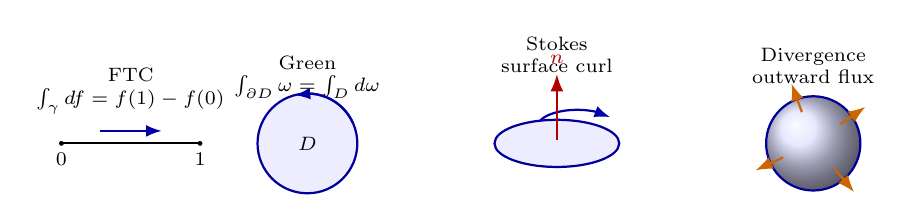
\begin{tikzpicture}[scale=0.88, every node/.style={font=\scriptsize}]
\begin{scope}
  \draw[thick] (0,0) -- (2,0);
  \fill (0,0) circle (0.035) node[below] {$0$};
  \fill (2,0) circle (0.035) node[below] {$1$};
  \draw[formarrow] (0.55,0.18) -- (1.45,0.18);
  \node[align=center] at (1,0.75) {FTC\\$\int_\gamma df=f(1)-f(0)$};
\end{scope}
\begin{scope}[xshift=3.55cm]
  \filldraw[region] (0,0) circle (0.72);
  \draw[formarrow] (25:0.72) arc (25:105:0.72);
  \node at (0,0) {$D$};
  \node[align=center] at (0,0.95) {Green\\$\int_{\partial D}\omega=\int_Dd\omega$};
\end{scope}
\begin{scope}[xshift=7.15cm]
  \filldraw[region] (0,0) ellipse (0.9 and 0.34);
  \draw[formarrow] (-0.25,0.32) arc (160:35:0.58 and 0.25);
  \draw[vector, red!70!black] (0,0.05) -- (0,1.0) node[above] {$n$};
  \node[align=center] at (0,1.28) {Stokes\\surface curl};
\end{scope}
\begin{scope}[xshift=10.85cm]
  \shade[ball color=blue!12] (0,0) circle (0.68);
  \draw[thick, blue!60!black] (0,0) circle (0.68);
  \foreach \a in {35,110,205,310}
    \draw[vector, orange!80!black] (\a:0.48) -- (\a:0.92);
  \node[align=center] at (0,1.12) {Divergence\\outward flux};
\end{scope}
\end{tikzpicture}
\visualcaption{The four named theorems are dimension-specific instances of the same Stokes pattern: integrate a form on the boundary, or integrate its exterior derivative on the region.}
\end{center}

\paragraph{The Stokes ladder.}
The four classical integral theorems form a single, ascending pattern: at each level, one integrates a $k$-form along the $k$-dimensional boundary, or one integrates its $d$-image over the $(k{+}1)$-dimensional region. This unified picture makes the abstraction transparent and explains why ``$d^2=0$'' is the same algebraic identity that lies behind $\nabla\times\nabla=0$ and $\nabla\cdot\nabla\times=0$.

\begin{center}
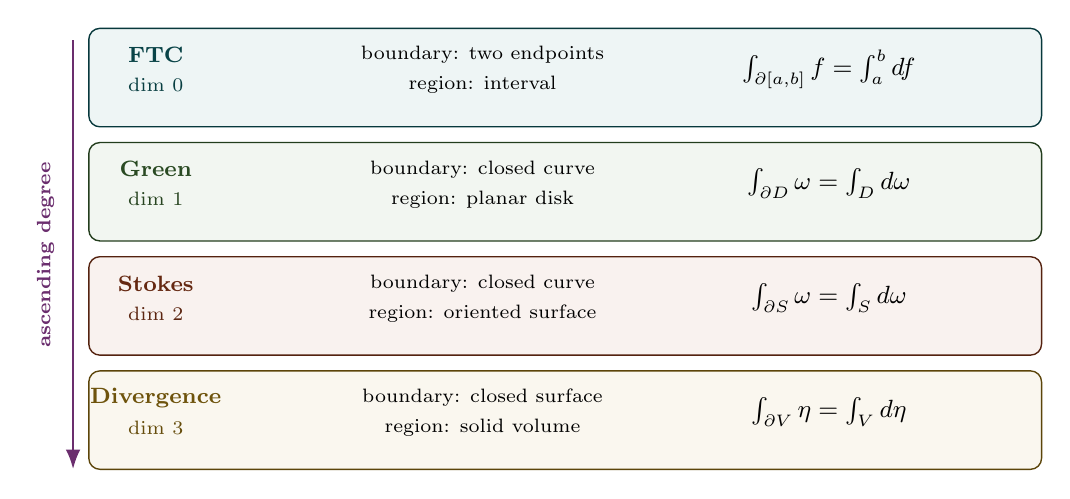
\begin{tikzpicture}[scale=1.0, every node/.style={font=\scriptsize}]
% Row 0: FTC
\begin{scope}[yshift=0cm]
  \fill[formteal!7, rounded corners=4pt] (-1.6,-0.55) rectangle (10.5,0.7);
  \draw[formteal!50!black, line width=0.5pt, rounded corners=4pt] (-1.6,-0.55) rectangle (10.5,0.7);
  \node[formteal!60!black, font=\bfseries\footnotesize] at (-0.75,0.36) {FTC};
  \node[formteal!55!black, font=\scriptsize] at (-0.75,-0.02) {dim 0};
  \node[font=\scriptsize] at (3.4,0.36) {boundary: two endpoints};
  \node[font=\scriptsize] at (3.4,-0.02) {region: interval};
  \node[font=\small] at (7.8,0.18) {$\int_{\partial[a,b]}f=\int_a^b df$};
\end{scope}
\begin{scope}[yshift=-1.45cm]
  \fill[formsage!7, rounded corners=4pt] (-1.6,-0.55) rectangle (10.5,0.7);
  \draw[formsage!50!black, line width=0.5pt, rounded corners=4pt] (-1.6,-0.55) rectangle (10.5,0.7);
  \node[formsage!60!black, font=\bfseries\footnotesize] at (-0.75,0.36) {Green};
  \node[formsage!55!black, font=\scriptsize] at (-0.75,-0.02) {dim 1};
  \node[font=\scriptsize] at (3.4,0.36) {boundary: closed curve};
  \node[font=\scriptsize] at (3.4,-0.02) {region: planar disk};
  \node[font=\small] at (7.8,0.18) {$\int_{\partial D}\omega=\int_D d\omega$};
\end{scope}
\begin{scope}[yshift=-2.9cm]
  \fill[formrust!7, rounded corners=4pt] (-1.6,-0.55) rectangle (10.5,0.7);
  \draw[formrust!50!black, line width=0.5pt, rounded corners=4pt] (-1.6,-0.55) rectangle (10.5,0.7);
  \node[formrust!60!black, font=\bfseries\footnotesize] at (-0.75,0.36) {Stokes};
  \node[formrust!55!black, font=\scriptsize] at (-0.75,-0.02) {dim 2};
  \node[font=\scriptsize] at (3.4,0.36) {boundary: closed curve};
  \node[font=\scriptsize] at (3.4,-0.02) {region: oriented surface};
  \node[font=\small] at (7.8,0.18) {$\int_{\partial S}\omega=\int_S d\omega$};
\end{scope}
\begin{scope}[yshift=-4.35cm]
  \fill[formgold!7, rounded corners=4pt] (-1.6,-0.55) rectangle (10.5,0.7);
  \draw[formgold!50!black, line width=0.5pt, rounded corners=4pt] (-1.6,-0.55) rectangle (10.5,0.7);
  \node[formgold!60!black, font=\bfseries\footnotesize] at (-0.75,0.36) {Divergence};
  \node[formgold!55!black, font=\scriptsize] at (-0.75,-0.02) {dim 3};
  \node[font=\scriptsize] at (3.4,0.36) {boundary: closed surface};
  \node[font=\scriptsize] at (3.4,-0.02) {region: solid volume};
  \node[font=\small] at (7.8,0.18) {$\int_{\partial V}\eta=\int_V d\eta$};
\end{scope}
% Decorative vertical "spine"
\draw[doubleformarrow, formplum, line width=1pt] (-1.8,0.55) -- (-1.8,-4.9);
\node[formplum, font=\scriptsize\bfseries, rotate=90] at (-2.15,-2.18) {ascending degree};
\end{tikzpicture}
\visualcaption{The same Stokes equation lives at every level. Only the dimension and the geometric interpretation change; the algebra is identical.}
\end{center}

\windingnote{Each of the four named theorems collapses to ``$0=0$'' for the winding form $\omega$ on a region where it is exact (i.e.\ any simply-connected open subset of $\R^2\setminus\{0\}$): on such a region $\omega=d(\arg)$, and integrating around a closed loop gives the endpoint difference of $\arg$, which is zero because the endpoints coincide. The whole interest of $\omega$ is exactly the case where the region is \emph{not} simply connected: Green's theorem applied formally to a loop encircling the origin returns $\oint\omega=2\pi$, even though ``$d\omega=0$'' would suggest $\iint_D d\omega=0$. The contradiction is resolved by noticing that $\omega$ is not defined at the origin, so $D$ is not really a region for the form; instead one removes a small disk and recovers the same $\eps\to 0$ argument as in Problem~3. The integral theorems thus already \emph{hide} the residue theorem inside themselves, with the winding form as the prototype obstruction.}

\handsketch{%
\fill[handpaper] (-3.4,-1.85) rectangle (3.4,1.85);
\draw[hand] (-3.4,-1.85) rectangle (3.4,1.85);
% Left: simply connected region (Stokes works)
\begin{scope}[xshift=-1.85cm]
  \draw[handthick] plot[smooth cycle] coordinates {(-1.0,-0.8) (-0.8,0.5) (0.05,0.9) (0.9,0.7) (1.0,-0.5) (0.3,-0.9) (-0.6,-0.95)};
  \draw[handarrow] (35:0.7) arc (35:135:0.7);
  \node[handnote] at (0,1.2) {simply connected};
  \node[handnote] at (0,-1.25) {$\oint\omega=0$};
\end{scope}
% Right: punctured region (Stokes fails -> 2pi)
\begin{scope}[xshift=1.85cm]
  \draw[handthick] plot[smooth cycle] coordinates {(-1.0,-0.8) (-0.8,0.5) (0.05,0.9) (0.9,0.7) (1.0,-0.5) (0.3,-0.9) (-0.6,-0.95)};
  \fill[handink] (0,0) circle (0.04);
  \draw[handthick] (0,0) circle (0.18);
  \draw[handarrow] (40:0.85) arc (40:130:0.85);
  \node[handnote] at (0,1.2) {has a puncture};
  \node[handnote] at (0,-1.25) {$\oint\omega=2\pi$};
\end{scope}
\draw[hand, dashed, line width=0.3pt] (0,-1.5) -- (0,1.5);
}

\subsection*{Problem 4(a): Fundamental theorem of line integrals}

\solutionflow{path\\\(\gamma(t)=(t,t^2)\)}
{pull back\\\(df\)}
{endpoint difference\\\(f(\gamma(1))-f(\gamma(0))\)}
{Problem 4(a) is solved by comparing the direct line-integral computation with the endpoint form of the fundamental theorem.}

Throughout Problem 4(a) we use
\[
 f(x,y)=x^2y,
 \qquad
 \gamma(t)=(t,t^2),
 \qquad
 0\leq t\leq 1.
\]

\begin{center}
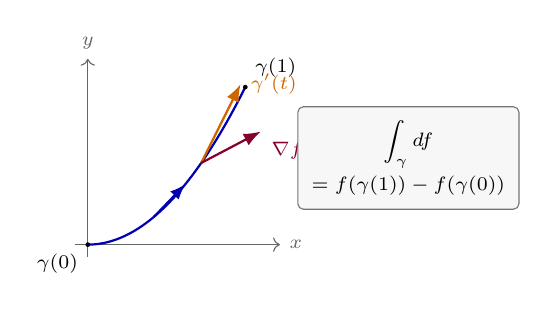
\begin{tikzpicture}[scale=2.0, every node/.style={font=\scriptsize}]
\draw[->, black!60] (-0.08,0) -- (1.22,0) node[right] {$x$};
\draw[->, black!60] (0,-0.08) -- (0,1.18) node[above] {$y$};
\draw[thick, blue!70!black, domain=0:1, samples=60, variable=\t] plot ({\t},{\t*\t});
\draw[formarrow, blue!70!black] (0.42,0.1764) -- (0.62,0.3844);
\fill (0,0) circle (0.015) node[below left] {$\gamma(0)$};
\fill (1,1) circle (0.015) node[above right] {$\gamma(1)$};
\coordinate (P) at (0.72,0.5184);
\draw[vector, orange!80!black] (P) -- ++(0.25,0.5) node[right] {$\gamma'(t)$};
\draw[vector, purple!70!black] (P) -- ++(0.38,0.2) node[below right] {$\nabla f$};
\node[visualnode, anchor=west] at (1.33,0.55)
{$\displaystyle \int_\gamma df$\\[2pt]
$=f(\gamma(1))-f(\gamma(0))$};
\end{tikzpicture}
\visualcaption{For the fundamental theorem calculation, the whole line integral collapses to endpoint data along the path $\gamma(t)=(t,t^2)$.}
\end{center}

\subsubsection*{Problem 4(a)-1: Compute the gradient $\nabla f$}

Differentiating $f(x,y)=x^2y$,
\[
 \nabla f=(\pd_xf,\pd_yf)=(2xy,\;x^2).
\]

\subsubsection*{Problem 4(a)-2: Compute the line integral $\int_\gamma\nabla f\cdot dr$}

The curve differential is
\[
 dr=\gamma'(t)\,dt=(1,2t)\,dt.
\]
Along the curve,
\[
 \nabla f(\gamma(t))=(2t\cdot t^2,\;t^2)=(2t^3,\;t^2).
\]
So
\[
 \nabla f(\gamma(t))\cdot\gamma'(t)
 =
 2t^3\cdot 1+t^2\cdot 2t=4t^3.
\]
Therefore
\[
 \int_\gamma\nabla f\cdot dr
 =
 \int_0^1 4t^3\,dt
 =
 1.
\]
The same computation in differential-form language uses
\[
 df=2xy\,dx+x^2\,dy.
\]
Along $\gamma(t)=(t,t^2)$, $dx=dt$ and $dy=2t\,dt$, so
\[
 \gamma^*(df)
 =
 2(t)(t^2)\,dt+t^2(2t\,dt)
 =
 4t^3\,dt,
\]
which is the same integrand as $\nabla f(\gamma(t))\cdot\gamma'(t)\,dt$.

\subsubsection*{Problem 4(a)-3: Compute $f(\gamma(1))-f(\gamma(0))$ and verify the theorem}

The endpoints are $\gamma(0)=(0,0)$ and $\gamma(1)=(1,1)$, so
\[
 f(\gamma(1))-f(\gamma(0))
 =
 f(1,1)-f(0,0)
 =
 1-0=1.
\]
The line integral computed in 4(a)-2 equals the endpoint difference computed here, so the fundamental theorem of line integrals
\[
 \int_\gamma\nabla f\cdot dr=f(\gamma(1))-f(\gamma(0))
\]
is verified for this example.

\subsection*{Problem 4(b): Green's theorem}

\solutionflow{\(\omega=Pdx+Qdy\)\\with \(P=-y,Q=x\)}
{differentiate\\\(d\omega=(Q_x-P_y)dx\,dy\)}
{disk area\\gives \(2\pi\)}
{Problem 4(b) is solved by turning the boundary integral into a constant area integral over the unit disk.}

Throughout Problem 4(b) we use
\[
 P(x,y)=-y,\qquad Q(x,y)=x,
\]
and let $D$ be the unit disk.

\subsubsection*{Problem 4(b)-1: Compute the boundary integral $\oint_{\partial D}(P\,dx+Q\,dy)$}

Use the positively oriented unit circle
\[
 x=\cos t,\qquad y=\sin t,\qquad 0\leq t\leq2\pi.
\]
Then
\[
 dx=-\sin t\,dt,\qquad dy=\cos t\,dt,
\]
so
\[
\begin{aligned}
 P\,dx+Q\,dy
 &=
 (-\sin t)(-\sin t\,dt)
 +(\cos t)(\cos t\,dt)\\
 &=(\sin^2t+\cos^2t)\,dt=dt.
\end{aligned}
\]
Therefore
\[
 \oint_{\partial D}(P\,dx+Q\,dy)
 =
 \int_0^{2\pi}dt
 =
 2\pi.
\]

\subsubsection*{Problem 4(b)-2: Compute $\iint_D(\partial_xQ-\partial_yP)\,dx\,dy$}

Differentiating,
\[
 \pd_xQ=1,\qquad \pd_yP=-1,
 \qquad\text{so}\qquad
 \pd_xQ-\pd_yP=2.
\]
The double integral is
\[
 \iint_D(\pd_xQ-\pd_yP)\,dx\,dy
 =
 \iint_D2\,dx\,dy
 =
 2\operatorname{Area}(D)
 =
 2\pi.
\]
In differential-form notation, $\omega=P\,dx+Q\,dy=-y\,dx+x\,dy$, and
\[
 d\omega
 =d(-y\,dx)+d(x\,dy)
 =-dy\wedge dx+dx\wedge dy
 =2\,dx\wedge dy,
\]
which represents the same integrand as $\pd_xQ-\pd_yP=2$.

\subsubsection*{Problem 4(b)-3: Verify Green's theorem}

The boundary integral computed in 4(b)-1 equals the double integral computed in 4(b)-2: both sides equal $2\pi$. Hence Green's theorem
\[
 \oint_{\partial D}(P\,dx+Q\,dy)
 =
 \iint_D(\pd_xQ-\pd_yP)\,dx\,dy
\]
is verified for this example.

\subsection*{Problem 4(c): Classical Stokes theorem}

\solutionflow{field\\\(F=(-y,x,0)\)}
{curl\\\(\nabla\times F=(0,0,2)\)}
{upward disk\\boundary is counterclockwise}
{Problem 4(c) is solved by matching upward surface orientation with the counterclockwise boundary orientation.}

Throughout Problem 4(c) we use the vector field $F=(-y,x,0)$ and let $S$ be the unit disk in the plane $z=0$ oriented by the upward unit normal $n=(0,0,1)$.

\subsubsection*{Problem 4(c)-1: Compute $\nabla\times F$}

Using the curl formula $\nabla\times F=(\pd_yF_3-\pd_zF_2,\;\pd_zF_1-\pd_xF_3,\;\pd_xF_2-\pd_yF_1)$ with $F_1=-y$, $F_2=x$, $F_3=0$,
\[
\begin{aligned}
 \nabla\times F
 &=
 \bigl(\pd_y0-\pd_zx,\;
 \pd_z(-y)-\pd_x0,\;
 \pd_xx-\pd_y(-y)\bigr)\\
 &=(0,\;0,\;1-(-1))=(0,0,2).
\end{aligned}
\]

\subsubsection*{Problem 4(c)-2: Compute the surface integral $\iint_S(\nabla\times F)\cdot n\,dS$}

On $S$,
\[
 (\nabla\times F)\cdot n=(0,0,2)\cdot(0,0,1)=2,
\]
so
\[
 \iint_S(\nabla\times F)\cdot n\,dS
 =
 \iint_S2\,dS
 =
 2\operatorname{Area}(S)=2\pi.
\]
In differential-form language, $\omega=-y\,dx+x\,dy$ and $d\omega=2\,dx\wedge dy$. On the disk $z=0$ with upward orientation, $dx\wedge dy$ is the positive area form, so $\int_Sd\omega=2\pi$ as well.

\subsubsection*{Problem 4(c)-3: Compute the boundary integral $\oint_{\partial S}F\cdot dr$}

The boundary orientation induced by the upward normal is counterclockwise. Parametrize it by
\[
 r(t)=(\cos t,\sin t,0),\qquad 0\leq t\leq2\pi.
\]
Then
\[
 r'(t)=(-\sin t,\cos t,0),
 \qquad
 F(r(t))=(-\sin t,\cos t,0),
\]
so
\[
 F(r(t))\cdot r'(t)=\sin^2t+\cos^2t=1.
\]
Therefore
\[
 \oint_{\partial S}F\cdot dr
 =
 \int_0^{2\pi}1\,dt
 =
 2\pi.
\]

\subsubsection*{Problem 4(c)-4: Verify Stokes' theorem}

The boundary integral computed in 4(c)-3 equals the surface integral computed in 4(c)-2: both equal $2\pi$. Hence the classical Stokes theorem
\[
 \oint_{\partial S}F\cdot dr
 =
 \iint_S(\nabla\times F)\cdot n\,dS
\]
is verified for this example.

\subsection*{Problem 4(d): Divergence theorem}

\solutionflow{field\\\(F=(x,y,z)\)}
{divergence\\\(\nabla\cdot F=3\)}
{unit ball volume\\and sphere flux give \(4\pi\)}
{Problem 4(d) is solved by comparing constant volume divergence with outward unit-sphere flux.}

Throughout Problem 4(d) we use $F=(x,y,z)$ and let $V$ be the unit ball, so $\partial V=S^2$ with outward normal.

\subsubsection*{Problem 4(d)-1: Compute the divergence $\nabla\cdot F$}

\[
 \nabla\cdot F=\pd_xx+\pd_yy+\pd_zz=1+1+1=3.
\]

\subsubsection*{Problem 4(d)-2: Compute the volume integral $\iiint_V(\nabla\cdot F)\,dV$}

\[
 \iiint_V(\nabla\cdot F)\,dV
 =
 \iiint_V3\,dV
 =
 3\operatorname{Vol}(V)
 =
 3\cdot\frac{4\pi}{3}
 =
 4\pi.
\]

\subsubsection*{Problem 4(d)-3: Compute the flux $\iint_{\partial V}F\cdot n\,dS$}

On the unit sphere $\partial V=S^2$, the outward unit normal at $(x,y,z)$ is $n=(x,y,z)$. Since $F=(x,y,z)$ as well,
\[
 F\cdot n=x^2+y^2+z^2=1
\]
on $S^2$. Hence
\[
 \iint_{\partial V}F\cdot n\,dS
 =
 \iint_{S^2}1\,dS
 =
 \operatorname{Area}(S^2)=4\pi.
\]
In differential-form language, the flux form associated to $F$ is
\[
 \eta=x\,dy\wedge dz+y\,dz\wedge dx+z\,dx\wedge dy,
\]
and
\[
\begin{aligned}
 d\eta
 &=
 dx\wedge dy\wedge dz
 +dy\wedge dz\wedge dx
 +dz\wedge dx\wedge dy\\
 &=
 3\,dx\wedge dy\wedge dz,
\end{aligned}
\]
using that $dy\wedge dz\wedge dx$ and $dz\wedge dx\wedge dy$ are cyclic reorderings of $dx\wedge dy\wedge dz$, hence have positive sign. This matches $\nabla\cdot F=3$.

\subsubsection*{Problem 4(d)-4: Verify the divergence theorem}

The volume integral from 4(d)-2 and the flux from 4(d)-3 both equal $4\pi$. Hence the divergence theorem
\[
 \iiint_V(\nabla\cdot F)\,dV
 =
 \iint_{\partial V}F\cdot n\,dS
\]
is verified for this example.

\section*{Problem 5: From $\bar z$-Derivatives to the Cauchy Integral Theorem}

\begin{intentrequirements}
\item \textbf{Intent.} Connect holomorphicity, the Cauchy--Riemann equations, Wirtinger derivatives, and Green's theorem, culminating in a proof of the Cauchy Integral Theorem for suitable planar domains.
\item \textbf{Required outputs.} Compute $\partial f/\partial\bar z$ for $f=u+iv$, show that $\partial f/\partial\bar z=0$ is equivalent to the Cauchy--Riemann equations, expand $f(z)\,dz$ into real and imaginary $1$-forms, and apply Green's theorem to both parts of the boundary integral.
\item \textbf{Required explanations.} Explain why a complex integral vanishes exactly when both its real and imaginary parts vanish. The two Green's theorem integrands must be explicitly identified and then killed by the Cauchy--Riemann equations.
\item \textbf{Common pitfalls to avoid.} Keep the signs straight in
\[
 f(z)\,dz=(u\,dx-v\,dy)+i(v\,dx+u\,dy).
\]
The sign in front of $v\,dy$ is negative because $i^2=-1$.
\end{intentrequirements}

Let
\[
 f(z)=u(x,y)+iv(x,y),
 \qquad
 z=x+iy.
\]

\begin{center}
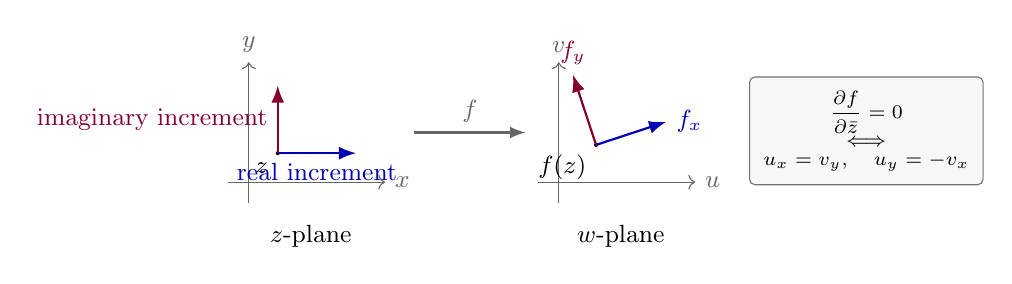
\begin{tikzpicture}[scale=1.05, every node/.style={font=\small}]
\begin{scope}
  \draw[->, black!60] (-0.25,0) -- (1.65,0) node[right] {$x$};
  \draw[->, black!60] (0,-0.25) -- (0,1.45) node[above] {$y$};
  \fill (0.35,0.35) circle (0.025) node[below left] {$z$};
  \draw[vector, blue!70!black] (0.35,0.35) -- ++(0.95,0) node[midway, below] {real increment};
  \draw[vector, purple!70!black] (0.35,0.35) -- ++(0,0.82) node[midway, left] {imaginary increment};
  \node[align=center] at (0.75,-0.65) {$z$-plane};
\end{scope}
\draw[formarrow, black!60] (2.0,0.6) -- node[above] {$f$} (3.35,0.6);
\begin{scope}[xshift=3.75cm]
  \draw[->, black!60] (-0.25,0) -- (1.65,0) node[right] {$u$};
  \draw[->, black!60] (0,-0.25) -- (0,1.45) node[above] {$v$};
  \fill (0.45,0.45) circle (0.025) node[below left] {$f(z)$};
  \draw[vector, blue!70!black] (0.45,0.45) -- ++(0.85,0.28) node[right] {$f_x$};
  \draw[vector, purple!70!black] (0.45,0.45) -- ++(-0.28,0.85) node[above] {$f_y$};
  \node[align=center] at (0.75,-0.65) {$w$-plane};
\end{scope}
\node[visualnode, anchor=west, font=\scriptsize] at (6.05,0.62)
{$\displaystyle \frac{\pd f}{\pd\bar z}=0$\\[2pt]
$\Longleftrightarrow$\\[-1pt]
$u_x=v_y,\quad u_y=-v_x$};
\end{tikzpicture}
\visualcaption{Holomorphicity says the derivative is independent of whether one approaches along the real or imaginary direction. The Wirtinger derivative packages that directional compatibility into one equation.}
\end{center}

\paragraph{Conformality and the Cauchy--Riemann equations.}
The Cauchy--Riemann equations say that the differential $df$ at every point is a rotation-scaling (a similarity matrix), so $f$ sends infinitesimal squares to infinitesimal squares and infinitesimal circles to infinitesimal circles. The Jacobian
\[
 Df=\begin{pmatrix} u_x & u_y \\ v_x & v_y \end{pmatrix}
 =\begin{pmatrix} a & -b \\ b & a \end{pmatrix}
\]
(with $a=u_x=v_y$, $b=-u_y=v_x$) is the real form of multiplication by $f'=a+ib$. Below, a small grid near a point is rotated and dilated, never sheared.

\begin{center}
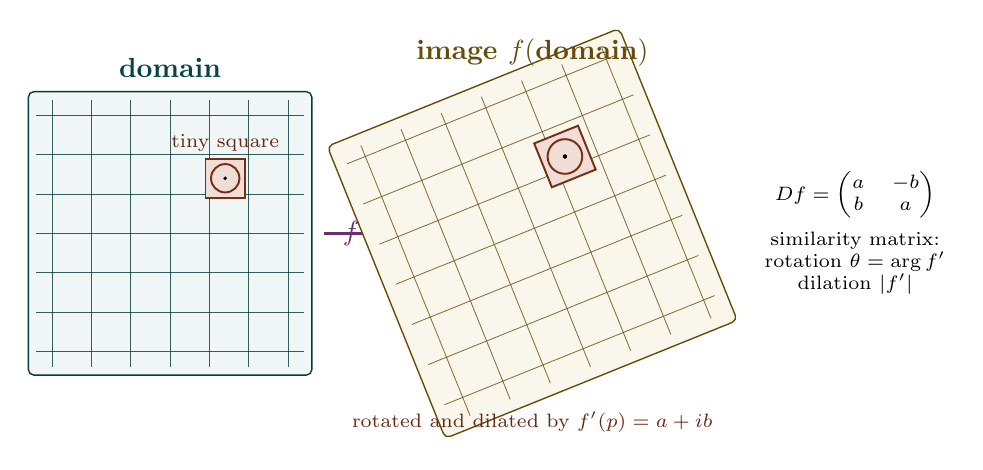
\begin{tikzpicture}[scale=1.0, every node/.style={font=\scriptsize}]
% Left panel: domain grid
\begin{scope}
  \filldraw[draw=formteal!50!black, fill=formteal!6, line width=0.5pt, rounded corners=2pt]
    (-1.8,-1.8) rectangle (1.8,1.8);
  \node[formteal!60!black, font=\bfseries] at (0,2.1) {domain};
  \foreach \x in {-1.5,-1,-0.5,0,0.5,1,1.5}
    \draw[formteal!50!black, line width=0.3pt, opacity=0.8] (\x,-1.7) -- (\x,1.7);
  \foreach \y in {-1.5,-1,-0.5,0,0.5,1,1.5}
    \draw[formteal!50!black, line width=0.3pt, opacity=0.8] (-1.7,\y) -- (1.7,\y);
  % highlight small square
  \filldraw[draw=formrust!70!black, fill=formrust!18, line width=0.7pt] (0.45,0.45) rectangle (0.95,0.95);
  \draw[formrust!70!black, line width=0.7pt] (0.7,0.7) circle (0.18);
  \fill[black] (0.7,0.7) circle (0.025);
  \node[formrust!60!black, font=\scriptsize] at (0.7,1.15) {tiny square};
\end{scope}
% Arrow with f
\node[formplum, font=\bfseries] at (2.3,0) {$f$};
\draw[->, formplum, line width=0.9pt] (1.95,0) -- (2.65,0);
% Right panel: image grid (rotated and scaled)
\begin{scope}[xshift=4.6cm, rotate=22]
  \filldraw[draw=formgold!55!black, fill=formgold!8, line width=0.5pt, rounded corners=2pt]
    (-2.0,-2.0) rectangle (2.0,2.0);
  \foreach \x in {-1.6,-1.05,-0.5,0.05,0.6,1.15,1.7}
    \draw[formgold!55!black, line width=0.3pt, opacity=0.8] (\x,-1.85) -- (\x,1.85);
  \foreach \y in {-1.6,-1.05,-0.5,0.05,0.6,1.15,1.7}
    \draw[formgold!55!black, line width=0.3pt, opacity=0.8] (-1.85,\y) -- (1.85,\y);
  \filldraw[draw=formrust!70!black, fill=formrust!18, line width=0.7pt]
    (0.45,0.45) rectangle (1.05,1.05);
  \draw[formrust!70!black, line width=0.7pt] (0.75,0.75) circle (0.22);
  \fill[black] (0.75,0.75) circle (0.028);
\end{scope}
\node[formgold!55!black, font=\bfseries] at (4.6,2.3) {image $f(\text{domain})$};
\node[formrust!60!black, font=\scriptsize] at (4.6,-2.4) {rotated and dilated by $f'(p)=a+ib$};
% Annotation
\node[font=\scriptsize, align=center] at (8.7,0)
{$Df=\begin{pmatrix} a & -b \\ b & a \end{pmatrix}$\\[4pt]
similarity matrix:\\rotation $\theta=\arg f'$\\dilation $|f'|$};
\end{tikzpicture}
\visualcaption{Cauchy--Riemann is the precise statement that $f$ acts on tangent spaces by complex multiplication, i.e.\ by similarity. Squares stay square, circles stay circular, angles are preserved.}
\end{center}

\subsection*{Problem 5(a): Compute $\pd f/\pd\bar z$}

\solutionflow{\(f=u+iv\)}
{use\\\(\pd_{\bar z}=\frac12(\pd_x+i\pd_y)\)}
{collect real and imaginary\\Cauchy--Riemann pieces}
{Problem 5(a) is solved by applying the Wirtinger operator and grouping the real and imaginary parts.}

The ordinary partial derivatives are
\[
 \frac{\pd f}{\pd x}=u_x+iv_x,
 \qquad
 \frac{\pd f}{\pd y}=u_y+iv_y.
\]
These follow by differentiating real and imaginary parts separately:
\[
 \frac{\pd}{\pd x}(u+iv)=u_x+i v_x,
 \qquad
 \frac{\pd}{\pd y}(u+iv)=u_y+i v_y.
\]
By definition,
\[
 \frac{\pd f}{\pd\bar z}
 =
 \frac12
 \left(
 \frac{\pd f}{\pd x}
 +i\frac{\pd f}{\pd y}
 \right).
\]
Substitute the two partial derivatives:
\[
\begin{aligned}
 \frac{\pd f}{\pd\bar z}
 &=
 \frac12
 \left(
 u_x+iv_x+i(u_y+iv_y)
 \right)\\
 &=
 \frac12
 \left(
 u_x+iv_x+iu_y-v_y
 \right)\\
 &=
 \frac12
 \left(
 (u_x-v_y)+i(v_x+u_y)
 \right).
\end{aligned}
\]

\subsection*{Problem 5(b): Equivalence with the Cauchy--Riemann equations}

\solutionflow{\(\pd f/\pd\bar z=0\)}
{real part zero\\\(u_x=v_y\)}
{imaginary part zero\\\(u_y=-v_x\)}
{Problem 5(b) is solved by reading one complex equation as two real equations.}

The equation
\[
 \frac{\pd f}{\pd\bar z}=0
\]
is equivalent to saying that both its real part and imaginary part are zero:
\[
 u_x-v_y=0,
 \qquad
 v_x+u_y=0.
\]
Equivalently,
\[
 u_x=v_y,
 \qquad
 u_y=-v_x.
\]
These are exactly the Cauchy--Riemann equations.

For a holomorphic function, the same equations follow from direction independence of the complex derivative. Taking increments in the real direction gives
\[
 f'(z)=f_x=u_x+iv_x.
\]
Taking increments in the imaginary direction gives
\[
 f'(z)=\frac{1}{i}f_y=-i(u_y+iv_y)=v_y-iu_y.
\]
Here is that second line more explicitly. If $h=it$ with $t\in\R$, then
\[
 \frac{f(z+h)-f(z)}{h}
 =
 \frac{f(x,y+t)-f(x,y)}{it}
 =
 \frac{1}{i}\frac{f(x,y+t)-f(x,y)}{t}.
\]
Letting $t\to0$ gives $(1/i)f_y=-if_y$.
Equating these two expressions gives
\[
 u_x=v_y,\qquad v_x=-u_y,
\]
which is the same system. Hence holomorphicity implies
\[
 \frac{\pd f}{\pd\bar z}=0.
\]

\subsection*{Problem 5(c): Express $f(z)\,dz$ in real coordinates}

\solutionflow{\(f=u+iv\)\\\(dz=dx+i\,dy\)}
{multiply\\and separate \(1,i\)}
{real form plus\\\(i\) times imaginary form}
{Problem 5(c) is solved by expanding the complex product into two real \(1\)-forms.}

Since
\[
 dz=dx+i\,dy,
\]
we have
\[
\begin{aligned}
 f(z)\,dz
 &=(u+iv)(dx+i\,dy)\\
 &=u\,dx+iu\,dy+iv\,dx+i^2v\,dy\\
 &=(u\,dx-v\,dy)+i(v\,dx+u\,dy).
\end{aligned}
\]
Therefore
\[
 \oint_{\partial D}f(z)\,dz
 =
 \oint_{\partial D}(u\,dx-v\,dy)
 +
 i\oint_{\partial D}(v\,dx+u\,dy).
\]
This equation says that a complex line integral is just two real line integrals packaged together: the first integral is its real part, and the second integral is its imaginary part.

\subsection*{Problem 5(d): Apply Green's theorem}

\solutionflow{split\\\(\oint f\,dz=A+iB\)}
{apply Green\\to \(A\) and \(B\)}
{Cauchy--Riemann\\kills both integrands}
{Problem 5(d) is solved by reducing the complex integral theorem to two applications of Green's theorem.}

Apply Green's theorem to the real and imaginary parts separately.
This is allowed because $u$ and $v$ are $C^1$ when $f$ is holomorphic on a neighborhood of $D$ and $\partial D$ in the setting of the theorem.

\begin{center}
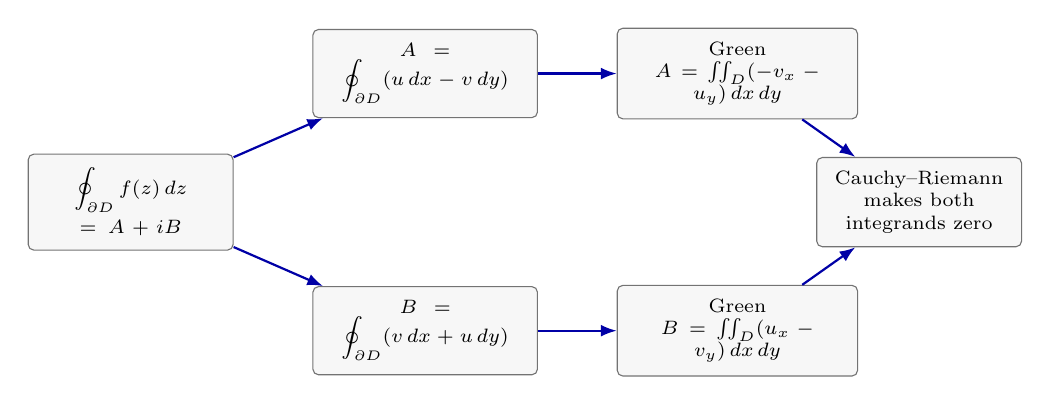
\begin{tikzpicture}[node distance=1.2cm, every node/.style={font=\scriptsize}]
\node[visualnode, text width=2.25cm] (int) {$\displaystyle \oint_{\partial D} f(z)\,dz$\\[2pt]$=A+iB$};
\node[visualnode, text width=2.5cm, above right=0.45cm and 1.0cm of int] (real) {$A=\displaystyle\oint_{\partial D}(u\,dx-v\,dy)$};
\node[visualnode, text width=2.5cm, below right=0.45cm and 1.0cm of int] (imag) {$B=\displaystyle\oint_{\partial D}(v\,dx+u\,dy)$};
\node[visualnode, text width=2.7cm, right=1.0cm of real] (greenr) {Green\\$A=\iint_D(-v_x-u_y)\,dx\,dy$};
\node[visualnode, text width=2.7cm, right=1.0cm of imag] (greeni) {Green\\$B=\iint_D(u_x-v_y)\,dx\,dy$};
\coordinate (greenmid) at ($(greenr)!0.5!(greeni)$);
\node[visualnode, text width=2.25cm, right=1.0cm of greenmid] (zero) {Cauchy--Riemann\\makes both\\integrands zero};
\draw[formarrow] (int) -- (real);
\draw[formarrow] (int) -- (imag);
\draw[formarrow] (real) -- (greenr);
\draw[formarrow] (imag) -- (greeni);
\draw[formarrow] (greenr) -- (zero);
\draw[formarrow] (greeni) -- (zero);
\end{tikzpicture}
\visualcaption{The proof of the Cauchy integral theorem is a split into two real Green's theorem computations, then a cancellation by the Cauchy--Riemann equations.}
\end{center}

For the first integral,
\[
 P=u,\qquad Q=-v.
\]
Thus
\[
\begin{aligned}
 \oint_{\partial D}(u\,dx-v\,dy)
 &=
 \iint_D
 \left(
 \frac{\pd(-v)}{\pd x}
 -
 \frac{\pd u}{\pd y}
 \right)\,dx\,dy\\
 &=
 \iint_D(-v_x-u_y)\,dx\,dy.
\end{aligned}
\]
For the second integral,
\[
 P=v,\qquad Q=u.
\]
Thus
\[
\begin{aligned}
 \oint_{\partial D}(v\,dx+u\,dy)
 &=
 \iint_D
 \left(
 \frac{\pd u}{\pd x}
 -
 \frac{\pd v}{\pd y}
 \right)\,dx\,dy\\
 &=
 \iint_D(u_x-v_y)\,dx\,dy.
\end{aligned}
\]
If $f$ is holomorphic, then the Cauchy--Riemann equations give
\[
 u_y=-v_x,
 \qquad
 u_x=v_y.
\]
Therefore
\[
 -v_x-u_y=0,
 \qquad
 u_x-v_y=0.
\]
Both double integrals vanish, so
\[
 \oint_{\partial D}f(z)\,dz=0.
\]
More explicitly,
\[
 \oint_{\partial D}f(z)\,dz
 =
 \iint_D(-v_x-u_y)\,dx\,dy
 +
 i\iint_D(u_x-v_y)\,dx\,dy.
\]
The real part vanishes because $u_y=-v_x$, and the imaginary part vanishes because $u_x=v_y$.
This is the Cauchy Integral Theorem for regions to which Green's theorem applies.

\windingnote{The Cauchy Integral Theorem $\oint_{\partial D}f\,dz=0$ is exactly the statement that the form $f\,dz$ is \emph{closed} ($d(f\,dz)=\partial_{\bar z}f\,d\bar z\wedge dz=0$ when $\partial_{\bar z}f=0$) and locally exact wherever $f$ is holomorphic. The simplest non-trivial holomorphic function with a singularity is $f(z)=1/z$, for which $f\,dz=dz/z$ has $\oint_{S^1}dz/z=2\pi i$. Decomposing into real and imaginary parts gives $dz/z=\tfrac{x\,dx+y\,dy}{x^2+y^2}+i\,\omega$ where the second piece is exactly the winding form. So CIT, on a region not enclosing $0$, is the statement $\oint\omega=0$ (the trivial side of Problem~2), while on a region enclosing $0$ it fails with discrepancy $2\pi i$ --- precisely the residue. The winding form is therefore the universal obstruction to CIT, and the residue is the universal correction.}

\handsketch{%
\fill[handpaper] (-3.5,-1.9) rectangle (3.5,1.9);
\draw[hand] (-3.5,-1.9) rectangle (3.5,1.9);
% Center: circle representing S^1
\draw[handthick] (0,0) circle (1.25);
\fill[handink] (0,0) circle (0.05);
\node[handnote] at (0,-0.25) {$0$};
% Radial spoke -- the radial part
\draw[handarrow, line width=0.55pt] (0,0) -- (35:1.25);
% Tangent spoke -- the angular (winding) part
\draw[handarrow, line width=0.85pt] (35:1.25) -- ++(125:0.65);
\coordinate (IOM) at ($(35:1.25)+(60:0.55)$);
\node[handnote] at (IOM) {$i\,\omega$};
\node[handnote] at (35:0.7) {$\frac{x\,dx+y\,dy}{x^2+y^2}$};
% Formula
\node[handnote] at (-2.45,1.5) {$\dfrac{dz}{z}=\dfrac{x\,dx+y\,dy}{x^{2}+y^{2}}+i\,\omega$};
\node[handnote] at (2.45,1.5) {$\oint_{S^1}\dfrac{dz}{z}=2\pi i$};
\node[handnote] at (2.45,1.05) {$=\text{(0)}+i(2\pi)$};
\node[handnote] at (0,-1.6) {radial $\perp$ angular};
}

\section*{Problem 6: Gaussian Curvature, Area Forms, and Euler Characteristic}

\begin{intentrequirements}
\item \textbf{Intent.} Compute geometric quantities from parametrizations and use Gauss--Bonnet to convert total curvature into Euler characteristic.
\item \textbf{Required outputs.} For the sphere, compute $X_\phi$, $X_\theta$, the first fundamental form, the area form, the normal, the second fundamental form, Gaussian curvature, total curvature, and $\chi(S^2)$. For the area-form comparison, compute the projected Jacobian and explain the graph correction factor. For the torus, compute $E,F,G$, $dA$, the outward normal, $e,f,g$, $K$, total curvature, and $\chi(T^2)$.
\item \textbf{Required explanations.} Explain what each coordinate measures: $\phi$ and $\theta$ on the sphere; $u$ around the small circle and $v$ around the central axis on the torus. Also explain why positive and negative curvature cancel on the torus.
\item \textbf{Common pitfalls to avoid.} Do not confuse projected $xy$-area with surface area. The sphere's surface area form requires a graph correction factor:
\[
 |\sin\phi\cos\phi|\,d\phi\,d\theta
 \quad\leadsto\quad
 \sin\phi\,d\phi\,d\theta.
\]
\end{intentrequirements}

\windingnote{The Gauss--Bonnet identity $\int_M K\,dA=2\pi\,\chi(M)$ is the most refined relative of the winding form's integral. To see the connection: the unit-normal field $N:M\to S^2$ is the Gauss map, and the pull-back $N^*(\text{area form on }S^2)$ equals $K\,dA$ up to the Jacobian of $N$. Hence $\int_M K\,dA$ is $4\pi\cdot\deg(N)$, i.e.\ $4\pi$ times the (integer) topological degree of the Gauss map --- the higher-dimensional cousin of the winding number. Dividing by $2\pi$ gives $\chi(M)$. So curvature integrals are \emph{winding integrals over the unit-normal sphere}, and the $2\pi$ that comes out is the same $2\pi$ from $\oint_{S^1}\omega=2\pi$.}

\handsketch{%
\fill[handpaper] (-3.4,-1.9) rectangle (3.4,1.9);
\draw[hand] (-3.4,-1.9) rectangle (3.4,1.9);
% Surface M (on the left)
\begin{scope}[xshift=-1.85cm]
  \draw[handthick] plot[smooth cycle] coordinates {(-1.1,-0.65) (-0.9,0.55) (0.0,0.85) (0.95,0.55) (1.1,-0.5) (0.4,-0.95) (-0.6,-0.95)};
  % Normal vectors on surface
  \foreach \xx/\yy/\dx/\dy in {-0.5/0.3/-0.3/0.45, 0.3/0.55/0.15/0.55, 0.7/-0.15/0.45/0.25, -0.2/-0.55/-0.05/-0.55}{
    \draw[handarrow] (\xx,\yy) -- ++(\dx,\dy);
  }
  \node[handnote] at (0,-1.3) {surface $M$};
\end{scope}
% Arrow for Gauss map
\draw[draw=handink, -{Latex[length=2.5mm]}, line width=0.8pt] (-0.5,0) -- (0.5,0);
\node[handnote] at (0,0.3) {$N$};
% Sphere S^2 on the right
\begin{scope}[xshift=1.85cm]
  \draw[handthick] (0,0) circle (1.05);
  \draw[draw=handink, line width=0.4pt, opacity=0.5] (0,0) ellipse (1.05 and 0.32);
  % Image of N — covering some part of S^2
  \draw[draw=handink, line width=0.55pt] plot[smooth cycle] coordinates {(-0.5,-0.3) (-0.45,0.4) (0.2,0.55) (0.6,0.3) (0.55,-0.25) (0.0,-0.5)};
  \fill[handink, opacity=0.18] plot[smooth cycle] coordinates {(-0.5,-0.3) (-0.45,0.4) (0.2,0.55) (0.6,0.3) (0.55,-0.25) (0.0,-0.5)};
  \node[handnote] at (0,-1.3) {$S^2$ (target)};
\end{scope}
\node[handnote] at (0,1.6) {Gauss map};
\node[handnote] at (0,-1.7) {$\int_M K\,dA=2\pi\chi(M)=4\pi\cdot\deg(N)$};
}

\subsection*{Problem 6(a): Geometry of the sphere in spherical coordinates}

\solutionflow{spherical map\\\(X(\phi,\theta)\)}
{first and second\\fundamental forms}
{\(K=1\), area \(4\pi\)\\so \(\chi(S^2)=2\)}
{Problem 6(a) is solved by computing the metric, curvature, total curvature, and then applying Gauss--Bonnet.}

Let
\[
 X(\phi,\theta)
 =
 (\sin\phi\cos\theta,\sin\phi\sin\theta,\cos\phi),
 \qquad
 0<\phi<\pi,\quad 0<\theta<2\pi.
\]

\begin{center}
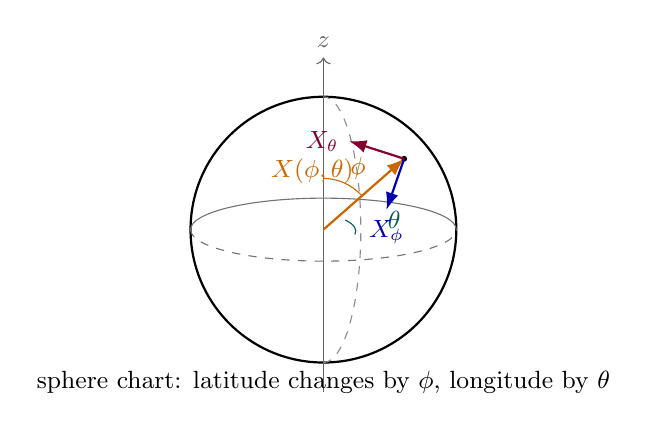
\begin{tikzpicture}[scale=1.25, every node/.style={font=\small}]
\draw[thick] (0,0) circle (1.35);
\draw[dashed, black!55] (-1.35,0) arc (180:360:1.35 and 0.32);
\draw[black!55] (1.35,0) arc (0:180:1.35 and 0.32);
\draw[dashed, black!45] (0,-1.35) arc (-90:90:0.38 and 1.35);
\draw[->, black!60] (0,-1.65) -- (0,1.75) node[above] {$z$};
\coordinate (P) at (0.82,0.72);
\draw[vector, orange!80!black] (0,0) -- (P) node[midway, above left] {$X(\phi,\theta)$};
\fill (P) circle (0.03);
\draw[thin, orange!80!black] (0,0.52) arc (90:42:0.52);
\node[orange!80!black] at (0.35,0.62) {$\phi$};
\draw[thin, teal!70!black] (0.32,-0.05) arc (-9:31:0.75 and 0.22);
\node[teal!70!black] at (0.72,0.1) {$\theta$};
\draw[vector, blue!70!black] (P) -- ++(-0.18,-0.52) node[below] {$X_\phi$};
\draw[vector, purple!70!black] (P) -- ++(-0.56,0.18) node[left] {$X_\theta$};
\node at (0,-1.55) {sphere chart: latitude changes by $\phi$, longitude by $\theta$};
\end{tikzpicture}
\visualcaption{The area factor $\sin\phi$ is the length of the longitude tangent $X_\theta$; it shrinks near the poles and is largest at the equator.}
\end{center}

\subsubsection*{Problem 6(a)-1: Compute the tangent vectors $X_\phi,X_\theta$}

Differentiating $X$ one variable at a time,
\[
 X_\phi=(\cos\phi\cos\theta,\cos\phi\sin\theta,-\sin\phi),
\]
\[
 X_\theta=(-\sin\phi\sin\theta,\sin\phi\cos\theta,0).
\]
For example,
\[
 \pd_\phi(\sin\phi\cos\theta)=\cos\phi\cos\theta,
 \qquad
 \pd_\theta(\sin\phi\cos\theta)=-\sin\phi\sin\theta;
\]
the variables not being differentiated are treated as constants.

\subsubsection*{Problem 6(a)-2: Compute $E,F,G$}

The coefficients of the first fundamental form are
\[
\begin{aligned}
 E&=\langle X_\phi,X_\phi\rangle\\
 &=\cos^2\phi(\cos^2\theta+\sin^2\theta)+\sin^2\phi\\
 &=\cos^2\phi+\sin^2\phi=1,
\end{aligned}
\]
\[
 F=\langle X_\phi,X_\theta\rangle=0,
\]
since
\[
\begin{aligned}
 \langle X_\phi,X_\theta\rangle
 &=
 (\cos\phi\cos\theta)(-\sin\phi\sin\theta)
 +(\cos\phi\sin\theta)(\sin\phi\cos\theta)
 +(-\sin\phi)(0)\\
 &=
 -\sin\phi\cos\phi\cos\theta\sin\theta
 +\sin\phi\cos\phi\sin\theta\cos\theta\\
 &=0,
\end{aligned}
\]
and
\[
\begin{aligned}
 G&=\langle X_\theta,X_\theta\rangle\\
 &=\sin^2\phi(\sin^2\theta+\cos^2\theta)\\
 &=\sin^2\phi.
\end{aligned}
\]

\subsubsection*{Problem 6(a)-3: Deduce the spherical area element $dA=\sqrt{EG-F^2}\,d\phi\,d\theta$}

From the values $E=1$, $F=0$, $G=\sin^2\phi$,
\[
 dA=\sqrt{EG-F^2}\,d\phi\,d\theta
 =
 \sqrt{\sin^2\phi}\,d\phi\,d\theta.
\]
Since $0<\phi<\pi$, we have $\sin\phi>0$, so the area form reduces to the standard form
\[
 dA=\sin\phi\,d\phi\,d\theta.
\]
Equivalently, one can compute the cross product $\|X_\phi\times X_\theta\|=\sin\phi$, which agrees with $\sqrt{EG-F^2}$ via the Lagrange identity
\[
 \|X_\phi\times X_\theta\|^2
 =
 \|X_\phi\|^2\|X_\theta\|^2-\langle X_\phi,X_\theta\rangle^2
 =
 EG-F^2.
\]

\subsubsection*{Problem 6(a)-4: Total area of the unit sphere}

Integrating the area form over the full range,
\[
\begin{aligned}
 \operatorname{Area}(S^2)
 &=
 \int_0^{2\pi}\int_0^\pi
 \sin\phi\,d\phi\,d\theta\\
 &=
 \int_0^{2\pi}\bigl[-\cos\phi\bigr]_0^\pi\,d\theta
 =
 \int_0^{2\pi}2\,d\theta
 =4\pi.
\end{aligned}
\]

\subsubsection*{Problem 6(a)-5: Compute the outward unit normal field $N$ and show $N=X$}

Since $X(\phi,\theta)$ lies on the unit sphere, $\|X(\phi,\theta)\|=1$. The sphere is the level set $x^2+y^2+z^2=1$; the gradient $\nabla(x^2+y^2+z^2)=2(x,y,z)$ is radial. After normalizing, the outward unit normal is the radial vector itself,
\[
 N=X.
\]

\subsubsection*{Problem 6(a)-6: Compute the second derivatives $X_{\phi\phi},X_{\phi\theta},X_{\theta\theta}$}

\[
 X_{\phi\phi}
 =
 (-\sin\phi\cos\theta,-\sin\phi\sin\theta,-\cos\phi)
 =
 -X,
\]
\[
 X_{\phi\theta}
 =
 (-\cos\phi\sin\theta,\cos\phi\cos\theta,0),
\]
\[
 X_{\theta\theta}
 =
 (-\sin\phi\cos\theta,-\sin\phi\sin\theta,0).
\]

\subsubsection*{Problem 6(a)-7: Compute $e,f,g$}

Using $N=X$,
\[
 e=\langle X_{\phi\phi},N\rangle=\langle -X,X\rangle=-\|X\|^2=-1,
\]
\[
\begin{aligned}
 f=\langle X_{\phi\theta},N\rangle
 &=(-\cos\phi\sin\theta)(\sin\phi\cos\theta)
 +(\cos\phi\cos\theta)(\sin\phi\sin\theta)+0\\
 &=0,
\end{aligned}
\]
and
\[
\begin{aligned}
 g=\langle X_{\theta\theta},N\rangle
 &=
 -\sin^2\phi\cos^2\theta-\sin^2\phi\sin^2\theta+0\\
 &=
 -\sin^2\phi(\cos^2\theta+\sin^2\theta)
 =-\sin^2\phi.
\end{aligned}
\]
The negative signs in $e$ and $g$ come from the choice of outward normal: the second-derivative vectors bend \emph{inward}, opposite to $N$. The Gaussian curvature uses the product $eg-f^2$, so the final curvature is still positive.

\subsubsection*{Problem 6(a)-8: Compute the Gaussian curvature $K$}

\[
 K=\frac{eg-f^2}{EG-F^2}
 =
 \frac{(-1)(-\sin^2\phi)-0}{1\cdot\sin^2\phi-0}
 =
 \frac{\sin^2\phi}{\sin^2\phi}
 =
 1.
\]
Since curvature is intrinsic, this value extends smoothly to the poles where the chart breaks down: the round unit sphere has $K\equiv 1$.

\subsubsection*{Problem 6(a)-9: Compute the total curvature $\int_{S^2}K\,dA$}

\[
\begin{aligned}
 \int_{S^2}K\,dA
 &=
 \int_0^{2\pi}\int_0^\pi
 1\cdot\sin\phi\,d\phi\,d\theta
 =4\pi.
\end{aligned}
\]

\subsubsection*{Problem 6(a)-10: Determine the Euler characteristic $\chi(S^2)$ via Gauss--Bonnet}

The Gauss--Bonnet formula
\[
 \int_MK\,dA=2\pi\chi(M)
\]
applied to $M=S^2$ gives
\[
 4\pi=2\pi\chi(S^2),
\qquad\text{so}\qquad
 \chi(S^2)=2.
\]

\subsubsection*{Problem 6(a)-11: Geometric explanation of $\chi(S^2)=2$}

Geometrically, the unit sphere bends the same positive amount everywhere ($K=1$). Because the sphere has area $4\pi$, the total curvature is $4\pi$. Gauss--Bonnet translates that positive total curvature into the positive Euler characteristic $\chi(S^2)=2$: a closed surface with everywhere-positive curvature must be topologically a sphere, and the magnitude of its Euler characteristic is governed by how much total bending it accumulates.

\begin{center}
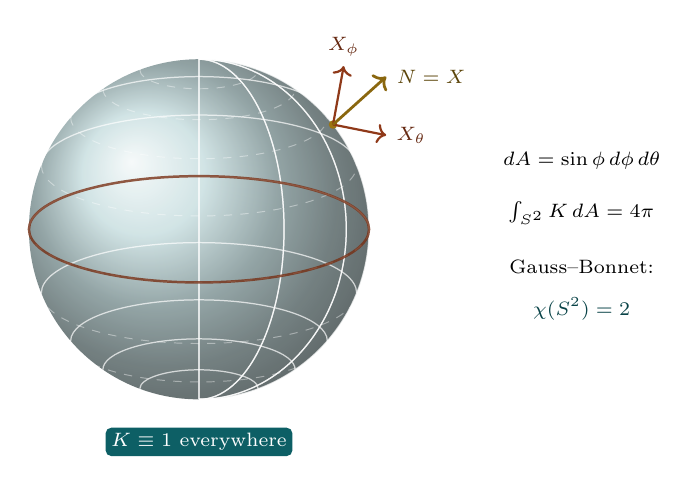
\begin{tikzpicture}[scale=1.35, every node/.style={font=\scriptsize}]
% Background gradient
\shade[ball color=formteal!30, opacity=0.85] (0,0) circle (1.6);
% Latitude lines (parallels)
\draw[white, line width=0.5pt, opacity=0.85] (1.6,0) arc (0:180:1.6 and 0.5);
\draw[dashed, white, line width=0.4pt, opacity=0.6] (-1.6,0) arc (180:360:1.6 and 0.5);
\foreach \yy in {0.6,1.05,1.32,1.5,-0.6,-1.05,-1.32,-1.5}{
  \pgfmathsetmacro\rxx{sqrt(2.56-\yy*\yy)}
  \draw[white, line width=0.45pt, opacity=0.7] ({\rxx},\yy) arc (0:180:{\rxx} and {0.32*\rxx});
  \draw[dashed, white, line width=0.35pt, opacity=0.4] ({-\rxx},\yy) arc (180:360:{\rxx} and {0.32*\rxx});
}
% Longitude lines (meridians)
\foreach \th in {0,30,60,90,120,150}{
  \pgfmathsetmacro\hor{cos(\th)*1.6}
  \draw[white, line width=0.45pt, opacity=0.75] (0,1.6) arc (90:-90:{abs(\hor)} and 1.6);
}
% Tangent vectors and normal at a point
\coordinate (P) at (38:1.6);
\fill[formgold!85!black] (P) circle (0.04);
\draw[->, formrust!85!black, line width=0.8pt] (P) -- ++(0.5,-0.1) node[right, formrust!60!black] {$X_\theta$};
\draw[->, formrust!85!black, line width=0.8pt] (P) -- ++(0.1,0.55) node[above, formrust!60!black] {$X_\phi$};
\draw[->, formgold!75!black, line width=1pt] (P) -- ++(0.5,0.45) node[right, formgold!50!black] {$N=X$};
% Equator highlighted
\draw[formrust!70!black, line width=0.9pt, opacity=0.8] (0,0) ellipse (1.6 and 0.5);
% Annotations
\node[font=\scriptsize, white, fill=formteal!85!black, rounded corners=2pt, inner sep=2pt] at (0,-2.0) {$K\equiv1$ everywhere};
\node[font=\scriptsize] at (3.6,0.65) {$dA=\sin\phi\,d\phi\,d\theta$};
\node[font=\scriptsize] at (3.6,0.15) {$\int_{S^2} K\,dA=4\pi$};
\node[font=\scriptsize] at (3.6,-0.35) {Gauss--Bonnet:};
\node[font=\scriptsize, formteal!60!black] at (3.6,-0.75) {$\chi(S^2)=2$};
\end{tikzpicture}
\visualcaption{The round sphere has uniform positive curvature. The area-weighted curvature density integrates to $4\pi$, which Gauss--Bonnet reads off as the Euler characteristic $\chi(S^2)=2$.}
\end{center}

\subsection*{Problem 6(b): Area form and change of variables}

\solutionflow{project to\\\((x,y)\)}
{Jacobian\\\(\sin\phi\cos\phi\)}
{graph factor\\recovers \(dA=\sin\phi\,d\phi\,d\theta\)}
{Problem 6(b) is solved by distinguishing projected area from surface area.}

Throughout Problem 6(b) we use the projection map
\[
 x=\sin\phi\cos\theta,
 \qquad
 y=\sin\phi\sin\theta,
\]
which sends the spherical parameters $(\phi,\theta)$ to the $xy$-projection of the corresponding point on the sphere.

\begin{center}
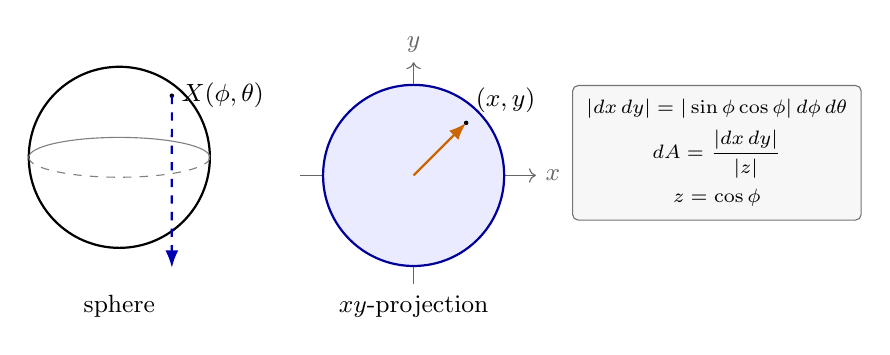
\begin{tikzpicture}[scale=1.15, every node/.style={font=\small}]
\begin{scope}
  \draw[thick] (0,0.2) circle (1.0);
  \draw[dashed, black!50] (-1,0.2) arc (180:360:1 and 0.22);
  \draw[black!50] (1,0.2) arc (0:180:1 and 0.22);
  \coordinate (P) at (0.58,0.88);
  \fill (P) circle (0.025) node[right] {$X(\phi,\theta)$};
  \draw[dashed, vector, blue!70!black] (P) -- (0.58,-1.02);
  \node at (0,-1.45) {sphere};
\end{scope}
\begin{scope}[xshift=3.25cm]
  \draw[->, black!60] (-1.25,0) -- (1.35,0) node[right] {$x$};
  \draw[->, black!60] (0,-1.2) -- (0,1.25) node[above] {$y$};
  \filldraw[fill=blue!8, draw=blue!60!black, thick] (0,0) circle (1.0);
  \fill (0.58,0.58) circle (0.025) node[above right] {$(x,y)$};
  \draw[vector, orange!80!black] (0,0) -- (0.58,0.58);
  \node at (0,-1.45) {$xy$-projection};
\end{scope}
\node[visualnode, anchor=west, font=\scriptsize] at (5.0,0.25)
{$|dx\,dy|=|\sin\phi\cos\phi|\,d\phi\,d\theta$\\[3pt]
$dA=\dfrac{|dx\,dy|}{|z|}$\\[3pt]
$z=\cos\phi$};
\end{tikzpicture}
\visualcaption{Projected area is not surface area. The graph factor $1/|z|$ repairs the flattening from the sphere to the $xy$-plane.}
\end{center}

\subsubsection*{Problem 6(b)-1: Compute the Jacobian $\partial(x,y)/\partial(\phi,\theta)$}

The Jacobian determinant is
\[
 \frac{\pd(x,y)}{\pd(\phi,\theta)}
 =
 \begin{vmatrix}
 \pd_\phi x & \pd_\theta x\\
 \pd_\phi y & \pd_\theta y
 \end{vmatrix}
 =
 \begin{vmatrix}
 \cos\phi\cos\theta & -\sin\phi\sin\theta\\
 \cos\phi\sin\theta & \sin\phi\cos\theta
 \end{vmatrix}.
\]
Expanding,
\[
\begin{aligned}
 \frac{\pd(x,y)}{\pd(\phi,\theta)}
 &=
 \cos\phi\sin\phi\cos^2\theta
 +
 \cos\phi\sin\phi\sin^2\theta\\
 &=
 \sin\phi\cos\phi.
\end{aligned}
\]

\subsubsection*{Problem 6(b)-2: Show $dA=\sin\phi\,d\phi\,d\theta$ agrees with the change-of-variables formula}

As a signed change of variables in the $xy$-plane, 6(b)-1 gives
\[
 dx\,dy=\sin\phi\cos\phi\,d\phi\,d\theta,
\qquad
 |dx\,dy|=|\sin\phi\cos\phi|\,d\phi\,d\theta.
\]
The surface-area form on the sphere is not merely the projected $xy$-area. On a hemisphere the sphere is a graph
\[
 z=\pm\sqrt{1-x^2-y^2},
\]
and the graph surface-area factor is
\[
 \sqrt{1+z_x^2+z_y^2}=\frac{1}{|z|}.
\]
Since $z=\cos\phi$,
\[
 dA=\frac{|dx\,dy|}{|z|}
 =
 \frac{|\sin\phi\cos\phi|}{|\cos\phi|}\,
 d\phi\,d\theta
 =
 \sin\phi\,d\phi\,d\theta.
\]
This agrees with the form $dA=\sqrt{EG-F^2}\,d\phi\,d\theta=\sin\phi\,d\phi\,d\theta$ obtained from the first fundamental form in 6(a)-3. The equator, where $\cos\phi=0$, is a measure-zero set where the projection to the $xy$-plane stops being a graph and does not affect the integral.

\subsubsection*{Problem 6(b)-3: Why the geometric area of the sphere is coordinate independent}

The two routes used above describe the same geometric area:
\begin{itemize}
\item the intrinsic first-fundamental-form route gives $dA=\sqrt{EG-F^2}\,d\phi\,d\theta=\sin\phi\,d\phi\,d\theta$;
\item the projection route gives $dA=|dx\,dy|/|z|=\sin\phi\,d\phi\,d\theta$.
\end{itemize}
Each formula carries its own Jacobian or graph factor, but after including the correct factor they represent the same geometric $2$-form $dA$ on the sphere. Integrating either expression over the full sphere yields $4\pi$, as computed in 6(a)-4. This is the precise sense in which the geometric area of the sphere does not depend on the chosen coordinates: it is a property of the $2$-form $dA$ itself, not of any particular chart.

\subsection*{Problem 6(c): Geometry of the torus}

\solutionflow{torus map\\\(X(u,v)\)}
{compute\\\(dA\) and \(K\)}
{\(K\,dA=\cos u\,du\,dv\)\\integrates to \(0\)}
{Problem 6(c) is solved by showing the positive and negative curvature contributions cancel over a full meridian.}

Let $R>r>0$ and
\[
 X(u,v)=((R+r\cos u)\cos v,\;(R+r\cos u)\sin v,\;r\sin u),
\]
with $0<u<2\pi$ and $0<v<2\pi$.
Here $u$ moves around the small circular cross-section of radius $r$, while $v$ rotates that cross-section around the central axis. The condition $R>r$ ensures the torus has no self-intersections and also ensures $R+r\cos u>0$.

\begin{center}
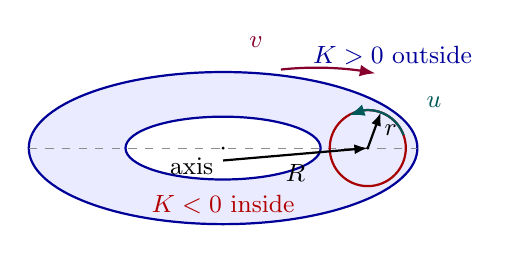
\begin{tikzpicture}[scale=1.05, every node/.style={font=\small}]
\fill[blue!8] (0,0) ellipse (2.35 and 0.92);
\fill[white] (0,0) ellipse (1.18 and 0.38);
\draw[thick, blue!60!black] (0,0) ellipse (2.35 and 0.92);
\draw[thick, blue!60!black] (0,0) ellipse (1.18 and 0.38);
\draw[dashed, black!45] (-2.35,0) -- (2.35,0);
\coordinate (C) at (1.75,0);
\draw[thick, red!65!black] (C) circle (0.46);
\fill (0,0) circle (0.02) node[below left] {axis};
\fill (C) circle (0.02);
\draw[tinyarrow] (0,-0.15) -- node[below] {$R$} (C);
\draw[tinyarrow] (C) -- node[right] {$r$} ++(70:0.46);
\draw[formarrow, teal!70!black] ($(C)+(20:0.46)$) arc (20:120:0.46);
\draw[formarrow, purple!70!black] (0.7,0.95) arc (110:55:1.25 and 0.38);
\node[teal!70!black] at (2.55,0.55) {$u$};
\node[purple!70!black] at (0.4,1.28) {$v$};
\node[blue!60!black] at (2.05,1.12) {$K>0$ outside};
\node[red!70!black] at (0,-0.68) {$K<0$ inside};
\end{tikzpicture}
\visualcaption{The parameter $u$ runs around a generating circle, while $v$ sweeps that circle around the central axis. The sign of $K$ follows the sign of $\cos u$: outside positive, inside negative.}
\end{center}

\subsubsection*{Problem 6(c)-1: Compute $E,F,G$ and deduce $dA$}

The first derivatives are
\[
 X_u=(-r\sin u\cos v,\;-r\sin u\sin v,\;r\cos u),
\]
\[
 X_v=(-(R+r\cos u)\sin v,\;(R+r\cos u)\cos v,\;0).
\]
Then
\[
\begin{aligned}
 E&=\langle X_u,X_u\rangle\\
 &=r^2\sin^2u\cos^2v+r^2\sin^2u\sin^2v+r^2\cos^2u\\
 &=r^2(\sin^2u+\cos^2u)=r^2,
\end{aligned}
\]
\[
\begin{aligned}
 F=\langle X_u,X_v\rangle
 &=(-r\sin u\cos v)(-(R+r\cos u)\sin v)\\
 &\quad+(-r\sin u\sin v)((R+r\cos u)\cos v)+0\\
 &=0,
\end{aligned}
\]
and $G=\langle X_v,X_v\rangle=(R+r\cos u)^2$. Therefore
\[
 dA=\sqrt{EG-F^2}\,du\,dv
 =
 r(R+r\cos u)\,du\,dv,
\]
where the positivity $R+r\cos u>0$ follows from $R>r$. As a check, the total surface area of the torus is
\[
 \int_0^{2\pi}\int_0^{2\pi}
 r(R+r\cos u)\,du\,dv
 =
 4\pi^2Rr,
\]
since the $\cos u$ term integrates to zero over a full period.

\subsubsection*{Problem 6(c)-2: Compute the Gaussian curvature $K(u,v)=\cos u/(r(R+r\cos u))$}

Choose the outward unit normal
\[
 N=(\cos u\cos v,\;\cos u\sin v,\;\sin u),
\]
which satisfies $\|N\|=1$, $\langle N,X_u\rangle=\langle N,X_v\rangle=0$, and at $u=0$ equals $(\cos v,\sin v,0)$, pointing away from the central axis. The second derivatives are
\[
 X_{uu}=(-r\cos u\cos v,-r\cos u\sin v,-r\sin u),
\]
\[
 X_{uv}=(r\sin u\sin v,-r\sin u\cos v,0),
\]
\[
 X_{vv}=(-(R+r\cos u)\cos v,-(R+r\cos u)\sin v,0).
\]
Hence
\[
 e=\langle X_{uu},N\rangle=-r,
 \qquad
 f=\langle X_{uv},N\rangle=0,
\]
and
\[
 g=\langle X_{vv},N\rangle=-(R+r\cos u)\cos u.
\]
Therefore
\[
\begin{aligned}
 K
 =
 \frac{eg-f^2}{EG-F^2}
 &=
 \frac{(-r)\bigl(-(R+r\cos u)\cos u\bigr)}
 {r^2(R+r\cos u)^2}\\
 &=
 \frac{\cos u}{r(R+r\cos u)}.
\end{aligned}
\]

\subsubsection*{Problem 6(c)-3: Compute $\int_{T^2}K\,dA$}

The crucial cancellation is that $K\,dA$ does not depend on the geometry of the cross-section:
\[
 K\,dA
 =
 \frac{\cos u}{r(R+r\cos u)}\cdot
 r(R+r\cos u)\,du\,dv
 =
 \cos u\,du\,dv.
\]
Hence
\[
\begin{aligned}
 \int_{T^2}K\,dA
 &=
 \int_0^{2\pi}\int_0^{2\pi}
 \cos u\,du\,dv\\
 &=
 \left(\int_0^{2\pi}\cos u\,du\right)
 \left(\int_0^{2\pi}dv\right)
 =0\cdot 2\pi=0.
\end{aligned}
\]

\subsubsection*{Problem 6(c)-4: Verify $\int_{T^2}K\,dA=2\pi\chi(T^2)$}

Gauss--Bonnet says $\int_{T^2}K\,dA=2\pi\chi(T^2)$. Combined with 6(c)-3,
\[
 0=2\pi\chi(T^2),
\qquad\text{so}\qquad
 \chi(T^2)=0.
\]
This vanishing also has a geometric interpretation: the outside of the torus has positive curvature where $\cos u>0$, while the inside has negative curvature where $\cos u<0$. The integral of $\cos u$ over a full period is zero, so the positive and negative contributions cancel exactly, in agreement with the topological fact $\chi(T^2)=0$.

\begin{center}
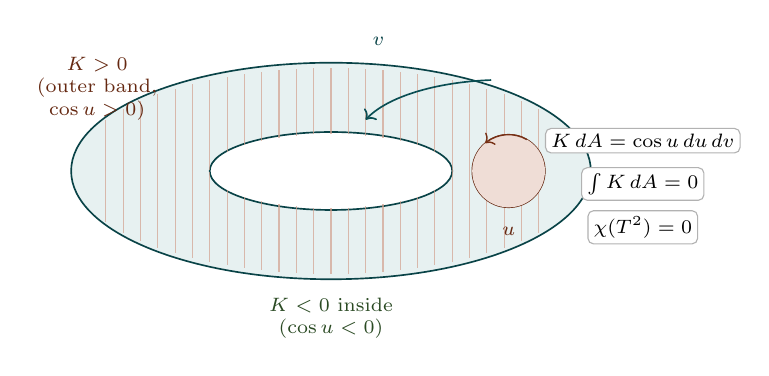
\begin{tikzpicture}[scale=1.1, every node/.style={font=\scriptsize}]
% Background outer ellipse
\fill[formteal!10] (0,0) ellipse (3.0 and 1.25);
\draw[formteal!60!black, line width=0.6pt] (0,0) ellipse (3.0 and 1.25);
% Inner ellipse (hole)
\fill[white] (0,0) ellipse (1.4 and 0.45);
\draw[formteal!60!black, line width=0.6pt] (0,0) ellipse (1.4 and 0.45);
% Color the outside region (K>0) and inside (K<0)
\foreach \xx in {-2.6,-2.4,...,2.6}{
  \pgfmathsetmacro\hh{0.95*sqrt(max(0,1-(\xx/3.0)*(\xx/3.0)))*1.25}
  \pgfmathsetmacro\hin{0.95*sqrt(max(0,1-(\xx/1.4)*(\xx/1.4)))*0.45}
  \pgfmathsetmacro\hindiff{\hh-\hin}
  \ifdim\hindiff pt>0pt
    % outer band: positive curvature
    \draw[formrust!50, line width=0.4pt, opacity=0.7] (\xx,\hin) -- (\xx,\hh);
    \draw[formrust!50, line width=0.4pt, opacity=0.7] (\xx,-\hin) -- (\xx,-\hh);
  \fi
}
% Crossing diameters meridian: little circle
\coordinate (C1) at (2.05,0);
\draw[formrust!60!black, line width=0.5pt] (C1) circle (0.42);
\fill[formrust!18] (C1) circle (0.42);
\draw[->, formrust!70!black, line width=0.5pt] ($(C1)+(60:0.42)$) arc (60:130:0.42);
\node[formrust!60!black, font=\scriptsize] at (2.05,-0.7) {$u$};
% Outer arrow v
\draw[->, formteal!70!black, line width=0.6pt] (1.85,1.05) arc (95:160:1.7 and 0.7);
\node[formteal!60!black, font=\scriptsize] at (0.55,1.5) {$v$};
% K positive label (outside)
\node[formrust!60!black, font=\scriptsize, align=center] at (-2.7,0.95) {$K>0$\\(outer band,\\$\cos u>0$)};
% K negative label (inside)
\node[formsage!60!black, font=\scriptsize, align=center] at (0,-1.7) {$K<0$ inside\\($\cos u<0$)};
% Annotate K dA = cos u
\node[font=\scriptsize, fill=white, rounded corners=2pt, inner sep=2pt, draw=black!30] at (3.6,0.35) {$K\,dA=\cos u\,du\,dv$};
\node[font=\scriptsize, fill=white, rounded corners=2pt, inner sep=2pt, draw=black!30] at (3.6,-0.15) {$\int K\,dA=0$};
\node[font=\scriptsize, fill=white, rounded corners=2pt, inner sep=2pt, draw=black!30] at (3.6,-0.65) {$\chi(T^2)=0$};
\end{tikzpicture}
\visualcaption{On the torus the positive curvature of the outer band exactly balances the negative curvature of the inner band. The total bending is zero, exposing the topological invariant $\chi(T^2)=0$.}
\end{center}

\section*{Problem 7: Euler Characteristic of $\CP^1$ and a Complex Torus}

\begin{intentrequirements}
\item \textbf{Intent.} Use conformal metrics and Gauss--Bonnet to compute Euler characteristics of two fundamental compact Riemann surfaces: $\CP^1$ and a complex torus.
\item \textbf{Required outputs.} For $\CP^1$, identify the Fubini--Study conformal factor $\lambda$, compute the area form, compute the Gaussian curvature, integrate $K\,dA$, and conclude $\chi(\CP^1)=2$. For the complex torus, show that the flat metric descends from $\C$, compute $K=0$, and conclude $\chi(T^2)=0$.
\item \textbf{Required explanations.} Explain why the integral over the affine chart $\C\subset\CP^1$ captures all of $\CP^1$: the missing point at infinity has area zero, and the density decays fast enough for convergence.
\item \textbf{Convention requirement.} Be explicit about the curvature normalization. With Wirtinger operators containing a factor $1/2$, the curvature formula must be normalized consistently to obtain $K=1$ for the round Fubini--Study metric used here.
\end{intentrequirements}

\windingnote{On $\CP^1$ the meromorphic $1$-form $dz/z$ extends globally with simple poles at $0$ and $\infty$ and residues $+1$ and $-1$ respectively. Its winding integral around either pole is $\pm 2\pi i$, and the sum of residues vanishes --- this is the first instance of the sum-of-residues theorem on a compact Riemann surface (final Problem~8). The same form on a complex torus $T^2=\C/\Lambda$ \emph{does not descend} (because $1/z$ is not periodic), but $dz$ itself does --- it is a nowhere-vanishing holomorphic $1$-form, so the canonical divisor on $T^2$ is trivial and $\deg K=2g-2=0$. The Gauss--Bonnet computations of this problem ($\chi(\CP^1)=2$, $\chi(T^2)=0$) match those degrees, with the $2\pi$ in $2\pi\chi$ being the same $2\pi$ from $\oint_{S^1}\omega=2\pi$.}

\handsketch{%
\fill[handpaper] (-3.4,-1.9) rectangle (3.4,1.9);
\draw[hand] (-3.4,-1.9) rectangle (3.4,1.9);
% Left: CP^1 sphere with two punctures
\begin{scope}[xshift=-1.7cm]
  \draw[handthick] (0,0) circle (1.15);
  \draw[draw=handink, line width=0.4pt, opacity=0.4] (0,0) ellipse (1.15 and 0.34);
  % Two punctures: 0 at south, infinity at north
  \fill[handink] (0,-1.15) circle (0.07);
  \node[handnote] at (-0.05,-1.4) {$0$};
  \node[handnote, anchor=west] at (0.13,-1.15) {$+1$};
  \draw[draw=handink, line width=0.55pt] (0,-1.15) circle (0.18);
  \draw[draw=handink, line width=0.45pt, -{Latex[length=1.5mm]}] ($(0,-1.15)+(20:0.18)$) arc (20:130:0.18);
  \fill[handink] (0,1.15) circle (0.07);
  \node[handnote] at (-0.1,1.4) {$\infty$};
  \node[handnote, anchor=west] at (0.13,1.15) {$-1$};
  \draw[draw=handink, line width=0.55pt] (0,1.15) circle (0.18);
  \draw[draw=handink, line width=0.45pt, -{Latex[length=1.5mm]}] ($(0,1.15)+(160:0.18)$) arc (160:50:-0.18);
  \node[handnote] at (0,-1.85) {$\CP^1$};
\end{scope}
% Right: torus with no poles for dz
\begin{scope}[xshift=1.7cm]
  \draw[handthick] (0,0) ellipse (1.1 and 0.6);
  \fill[white] (0,0) ellipse (0.5 and 0.2);
  \draw[draw=handink, line width=0.55pt] (0,0) ellipse (0.5 and 0.2);
  \node[handnote] at (0,-1.05) {$T^2$};
  \node[handnote] at (0,-1.45) {$dz$ nowhere vanishes};
  \node[handnote] at (0,-1.85) {$\deg K=0$};
\end{scope}
\node[handnote] at (-1.7,1.7) {$dz/z$: $\;\;+1\;\;-1$};
\node[handnote] at (1.7,1.7) {$dz$: no poles};
}

\begin{center}
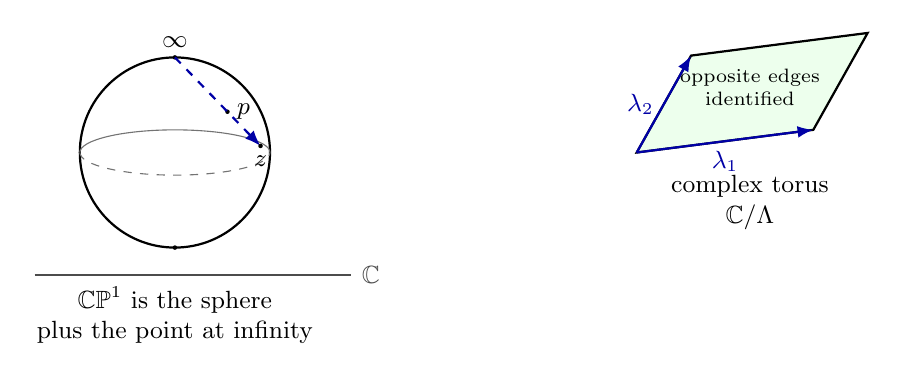
\begin{tikzpicture}[scale=1.15, every node/.style={font=\small}]
\begin{scope}
  \draw[thick] (0,0) circle (1.05);
  \draw[dashed, black!55] (-1.05,0) arc (180:360:1.05 and 0.25);
  \draw[black!55] (1.05,0) arc (0:180:1.05 and 0.25);
  \coordinate (N) at (0,1.05);
  \coordinate (S) at (0,-1.05);
  \coordinate (P) at (0.58,0.45);
  \fill (N) circle (0.025) node[above] {$\infty$};
  \fill (S) circle (0.025);
  \fill (P) circle (0.025) node[right] {$p$};
  \draw[thick, black!70] (-1.55,-1.35) -- (1.95,-1.35) node[right] {$\C$};
  \draw[dashed, formarrow] (N) -- ($(N)!1.63!(P)$);
  \fill ($(N)!1.63!(P)$) circle (0.025) node[below] {$z$};
  \node[align=center] at (0,-1.8) {$\CP^1$ is the sphere\\plus the point at infinity};
\end{scope}
\begin{scope}[xshift=5.1cm]
  \draw[thick, fill=green!7] (0,0) -- (1.95,0.25) -- (2.55,1.32) -- (0.6,1.07) -- cycle;
  \draw[formarrow] (0,0) -- node[below] {$\lambda_1$} (1.95,0.25);
  \draw[formarrow] (0,0) -- node[left] {$\lambda_2$} (0.6,1.07);
  \draw[dashed] (1.95,0.25) -- (2.55,1.32);
  \draw[dashed] (0.6,1.07) -- (2.55,1.32);
  \node[align=center] at (1.25,-0.55) {complex torus\\$\C/\Lambda$};
  \node[font=\scriptsize, align=center] at (1.25,0.72) {opposite edges\\identified};
\end{scope}
\end{tikzpicture}
\visualcaption{The two surfaces in this problem have different geometric models: $\CP^1$ is the Riemann sphere with the Fubini--Study metric, while a complex torus is a flat parallelogram quotient.}
\end{center}

\subsection*{Problem 7(a): Complex coordinates on $\CP^1$}

\solutionflow{Fubini--Study metric\\\(ds^2=\lambda|dz|^2\)}
{identify\\\(\lambda=\frac{4}{(1+|z|^2)^2}\)}
{area form\\\(dA=\lambda\,dx\,dy\)}
{Problem 7(a) is solved by reading the conformal factor directly from the metric.}

The Fubini--Study metric is
\[
 ds^2=\frac{4}{(1+|z|^2)^2}|dz|^2.
\]
Thus
\[
 \lambda(z,\bar z)=\frac{4}{(1+|z|^2)^2}.
\]
The area form is
\[
 dA=\lambda\,dx\,dy
 =
 \frac{4}{(1+|z|^2)^2}\,dx\,dy.
\]
Since
\[
 dx\,dy=\frac{i}{2}\,dz\wedge d\bar z,
\]
we can also write
\[
 dA=
 \frac{i}{2}\lambda\,dz\wedge d\bar z
 =
 \frac{2i}{(1+|z|^2)^2}\,dz\wedge d\bar z.
\]

\begin{center}
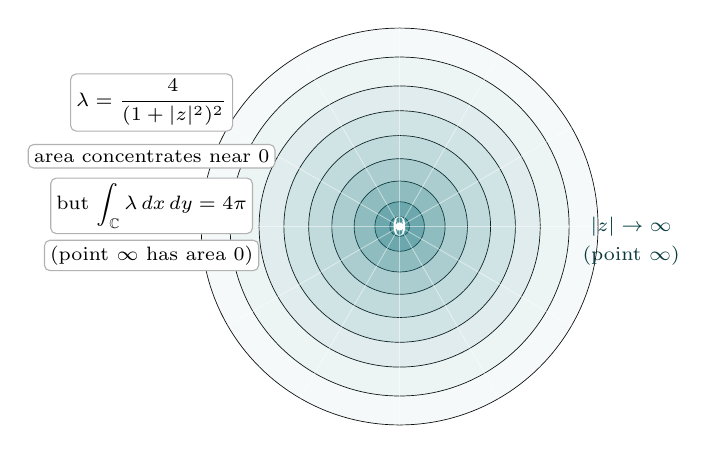
\begin{tikzpicture}[scale=1.05, every node/.style={font=\scriptsize}]
% Fubini-Study density rendered as nested rings
\foreach \r/\op in {2.4/4,2.05/8,1.7/13,1.4/19,1.1/26,0.82/35,0.55/47,0.3/62,0.12/75}{
  \filldraw[draw=formteal!\op!black, fill=formteal!\op, line width=0.25pt, opacity=0.95] (0,0) circle (\r);
}
\fill[white] (0,0) circle (0.05);
% Radial grid
\foreach \th in {0,30,...,330}{
  \draw[white, line width=0.3pt, opacity=0.5] (0,0) -- (\th:2.4);
}
% Annotate the affine chart and infinity
\node[white, font=\bfseries] at (0,0) {$0$};
\node[font=\scriptsize, formteal!55!black] at (2.8,0) {$|z|\to\infty$};
\node[font=\scriptsize, formteal!50!black] at (2.8,-0.35) {(point $\infty$)};
% Area density label
\node[font=\scriptsize, fill=white, rounded corners=2pt, inner sep=2pt, draw=black!30] at (-3.0,1.5)
{$\lambda=\dfrac{4}{(1+|z|^2)^2}$};
\node[font=\scriptsize, fill=white, rounded corners=2pt, inner sep=2pt, draw=black!30] at (-3.0,0.85)
{area concentrates near $0$};
\node[font=\scriptsize, fill=white, rounded corners=2pt, inner sep=2pt, draw=black!30] at (-3.0,0.25)
{but $\displaystyle\int_{\C}\lambda\,dx\,dy=4\pi$};
\node[font=\scriptsize, fill=white, rounded corners=2pt, inner sep=2pt, draw=black!30] at (-3.0,-0.35)
{(point $\infty$ has area $0$)};
\end{tikzpicture}
\visualcaption{The Fubini--Study area density $\lambda$ is brightest at the origin and decays as $|z|^{-4}$, integrating to the total area $4\pi$ of the Riemann sphere. The point at infinity is the limiting outer edge but contributes measure zero.}
\end{center}

\subsection*{Problem 7(b): Gaussian curvature of $\CP^1$}

\solutionflow{\(\lambda=\frac{4}{(1+z\bar z)^2}\)}
{differentiate\\\(\log\lambda\)}
{curvature formula\\gives \(K=1\)}
{Problem 7(b) is solved by applying the conformal curvature formula to the Fubini--Study factor.}

We compute with
\[
 \lambda=\frac{4}{(1+z\bar z)^2}.
\]
Since the metric is conformal to the Euclidean metric, all the curvature information is contained in the scalar conformal factor $\lambda$.
Then
\[
 \log\lambda=\log4-2\log(1+z\bar z).
\]
First,
\[
 \pd_z\log(1+z\bar z)
 =
 \frac{\bar z}{1+z\bar z}.
\]
Next,
\[
\begin{aligned}
 \pd_{\bar z}
 \left(
 \frac{\bar z}{1+z\bar z}
 \right)
 &=
 \frac{(1+z\bar z)-z\bar z}{(1+z\bar z)^2}\\
 &=
 \frac{1}{(1+|z|^2)^2}.
\end{aligned}
\]
Therefore
\[
 \pd_z\pd_{\bar z}\log\lambda
 =
 -\frac{2}{(1+|z|^2)^2}.
\]
The constant $\log4$ disappears because derivatives of constants are zero. The remaining calculation is the complex-coordinate version of differentiating a radial function.

With the Wirtinger operators as defined in the exam,
\[
 \pd_z\pd_{\bar z}=\frac14(\pd_x^2+\pd_y^2).
\]
Indeed,
\[
 \pd_z\pd_{\bar z}
 =
 \frac14(\pd_x-i\pd_y)(\pd_x+i\pd_y)
 =
 \frac14(\pd_x^2+\pd_y^2),
\]
because the mixed terms cancel:
\[
 i\pd_x\pd_y-i\pd_y\pd_x=0
\]
for smooth functions.
For a metric $ds^2=\lambda|dz|^2$, the standard curvature formula in this normalization is
\[
 K=-\frac{2}{\lambda}\pd_z\pd_{\bar z}\log\lambda.
\]
Thus
\[
\begin{aligned}
 K
 &=
 -\frac{2}{4/(1+|z|^2)^2}
 \left(
 -\frac{2}{(1+|z|^2)^2}
 \right)\\
 &=1.
\end{aligned}
\]

\emph{Convention note.} The revised PDF prints the curvature formula as
$K=-\lambda^{-1}\pd\bar\pd\log\lambda$ while also defining
$\pd,\bar\pd$ with the factor $1/2$. Taken literally, those two displayed conventions give $K=1/2$ here. The computation above uses the standard matching normalization, which is the one consistent with the exam's requested conclusion $K=1$ and with Gauss--Bonnet for the round unit sphere.

\subsection*{Problem 7(c): Euler characteristic of $\CP^1$}

\solutionflow{\(K=1\)}
{polar integral\\of \(dA\) over \(\C\)}
{Gauss--Bonnet\\\(\chi(\CP^1)=2\)}
{Problem 7(c) is solved by integrating the Fubini--Study area density and applying Gauss--Bonnet.}

Since $K=1$,
\[
 \int_{\CP^1}K\,dA
 =
 \int_{\C}
 \frac{4}{(1+|z|^2)^2}\,dx\,dy.
\]
Using polar coordinates $z=re^{i\theta}$,
\[
\begin{aligned}
 \int_{\CP^1}K\,dA
 &=
 \int_0^{2\pi}\int_0^\infty
 \frac{4}{(1+r^2)^2}r\,dr\,d\theta.
\end{aligned}
\]

\begin{center}
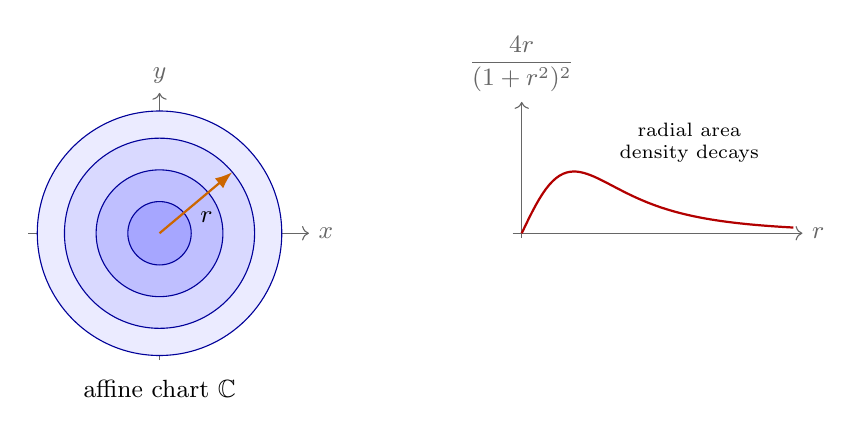
\begin{tikzpicture}[scale=1.15, every node/.style={font=\small}]
\begin{scope}
  \draw[->, black!60] (-1.45,0) -- (1.65,0) node[right] {$x$};
  \draw[->, black!60] (0,-1.4) -- (0,1.55) node[above] {$y$};
  \foreach \r/\c in {1.35/blue!8,1.05/blue!15,0.7/blue!25,0.35/blue!35}
    \filldraw[draw=blue!60!black, fill=\c] (0,0) circle (\r);
  \node at (0.52,0.18) {$r$};
  \draw[vector, orange!80!black] (0,0) -- (40:1.05);
  \node at (0,-1.72) {affine chart $\C$};
\end{scope}
\begin{scope}[xshift=4.0cm]
  \draw[->, black!60] (-0.1,0) -- (3.1,0) node[right] {$r$};
  \draw[->, black!60] (0,-0.05) -- (0,1.45) node[above] {$\dfrac{4r}{(1+r^2)^2}$};
  \draw[thick, red!70!black, domain=0:3, samples=80, variable=\r]
    plot ({\r},{2.1*\r/((1+\r*\r)*(1+\r*\r))});
  \node[font=\scriptsize, align=center] at (1.85,1.0) {radial area\\density decays};
\end{scope}
\end{tikzpicture}
\visualcaption{The $\CP^1$ integral becomes a polar integral over all radii. The conformal factor decays fast enough that the point at infinity contributes finite total area.}
\end{center}
For the radial integral, let $s=1+r^2$, so $ds=2r\,dr$:
\[
\begin{aligned}
 \int_0^\infty\frac{4r}{(1+r^2)^2}\,dr
 &=
 2\int_1^\infty s^{-2}\,ds\\
 &=
 2.
\end{aligned}
\]
Therefore
\[
 \int_{\CP^1}K\,dA=2\pi\cdot2=4\pi.
\]
This integral is over the single affine chart $\C\subset\CP^1$. The missing point at infinity has area zero, and the integrand decays like $r^{-4}$ while the polar area element contributes only $r\,dr\,d\theta$, so the improper integral converges.
By Gauss--Bonnet,
\[
 4\pi=2\pi\chi(\CP^1),
\]
so
\[
 \chi(\CP^1)=2.
\]

\subsection*{Problem 7(d): Complex torus}

\solutionflow{quotient\\\(T^2=\C/\Lambda\)}
{translations preserve\\\(|dz|^2\)}
{flat area form\\\(dA=dx\,dy\)}
{Problem 7(d) is solved by descending the Euclidean metric from the plane to the lattice quotient.}

Let
\[
 T^2=\C/\Lambda
\]
be a complex torus. The flat metric is
\[
 ds^2=|dz|^2.
\]
The quotient map $\C\to\C/\Lambda$ identifies points that differ by lattice vectors. Translations preserve the Euclidean metric $|dz|^2$, so this metric descends from $\C$ to the quotient torus.
Thus
\[
 \lambda=1.
\]
The associated area form is
\[
 dA=\lambda\,dx\,dy=dx\,dy.
\]
Equivalently,
\[
 dA=\frac{i}{2}\,dz\wedge d\bar z.
\]
On the quotient $\C/\Lambda$, this descends to the usual Euclidean area form on a fundamental parallelogram.

\subsection*{Problem 7(e): Gaussian curvature of the complex torus}

\solutionflow{\(\lambda=1\)}
{\(\log\lambda=0\)}
{\(K=0\)\\so \(\chi(T^2)=0\)}
{Problem 7(e) is solved by observing that the descended metric is flat.}

Since
\[
 \lambda=1,
\]
we have
\[
 \log\lambda=0.
\]
Therefore
\[
 \pd\bar\pd\log\lambda=0.
\]
The curvature is
\[
 K=0.
\]
Consequently,
\[
 \int_{T^2}K\,dA=0.
\]
Gauss--Bonnet gives
\[
 0=2\pi\chi(T^2),
\]
so
\[
 \chi(T^2)=0.
\]

\section*{Problem 8: Partition of Unity on $S^2$ and Integration}

\begin{intentrequirements}
\item \textbf{Intent.} Use a partition-of-unity style decomposition to compute the total area of the sphere by integrating local chart expressions.
\item \textbf{Required outputs.} Verify nonnegativity and the identity $\phi_N+\phi_S=1$, compute the local stereographic expressions for $\phi_N$ and $\phi_S$, integrate each weighted term in polar coordinates, and add the two contributions to recover $4\pi$.
\item \textbf{Required explanations.} Explain the role of stereographic coordinates and why both local integrals reduce to the same radial integral
\[
 \int_0^\infty \frac{4r}{(1+r^2)^3}\,dr.
\]
\item \textbf{Technical caveat.} Address the support issue carefully. With the strict support definition, the displayed functions are not literally subordinate to the stated open cover, but they vanish at the missing poles and are sufficient for the integral computation because single points have measure zero.
\end{intentrequirements}

\windingnote{The total area $4\pi=2\pi\cdot 2$ recovered here matches Gauss--Bonnet, since $\chi(S^2)=2$ and $K\equiv 1$. It also matches the winding-form story: stereographic coordinates make $S^2\setminus\{N\}\cong\C$, and the area integral splits into two equal halves $2\pi$ each --- mirroring the way $\oint_{S^1}\omega=2\pi$ splits into an upper-semicircle and a lower-semicircle contribution of $\pi$ each in Problem~2(b). The partition functions $\varphi_N,\varphi_S$ play, for areas, the role that the angular cutoffs play for the winding integral: they remove the singular pole from each chart in turn while keeping the total geometric content intact.}

\handsketch{%
\fill[handpaper] (-3.4,-1.9) rectangle (3.4,1.9);
\draw[hand] (-3.4,-1.9) rectangle (3.4,1.9);
% Globe with upper and lower hemisphere shaded
\draw[handthick] (0,0) circle (1.45);
\draw[draw=handink, line width=0.4pt, opacity=0.5] (0,0) ellipse (1.45 and 0.45);
% Upper hemi-shading (north chart)
\fill[handink, opacity=0.10] (1.45,0) arc (0:180:1.45) -- cycle;
% Lower hemi shading (south chart)
\fill[handsepia, opacity=0.13] (-1.45,0) arc (180:360:1.45) -- cycle;
% North pole and south pole
\fill[handink] (0,1.45) circle (0.06);
\node[handnote] at (0.15,1.55) {N};
\fill[handink] (0,-1.45) circle (0.06);
\node[handnote] at (0.15,-1.55) {S};
% Sum equals 1
\node[handnote] at (0,0) {$\varphi_N+\varphi_S=1$};
% labels
\node[handnote] at (-2.4,1.5) {$U_N$ chart};
\node[handnote] at (-2.4,1.05) {$\int\varphi_N\,dA=2\pi$};
\node[handnote] at (2.4,-1.05) {$U_S$ chart};
\node[handnote] at (2.4,-1.5) {$\int\varphi_S\,dA=2\pi$};
\node[handnote] at (0,-1.85) {total $=4\pi$};
}

Let
\[
 U_N=S^2\setminus\{(0,0,1)\},
 \qquad
 U_S=S^2\setminus\{(0,0,-1)\}.
\]
The functions are
\[
 \phi_N(x,y,z)=\frac{1-z}{2},
 \qquad
 \phi_S(x,y,z)=\frac{1+z}{2}.
\]

\begin{center}
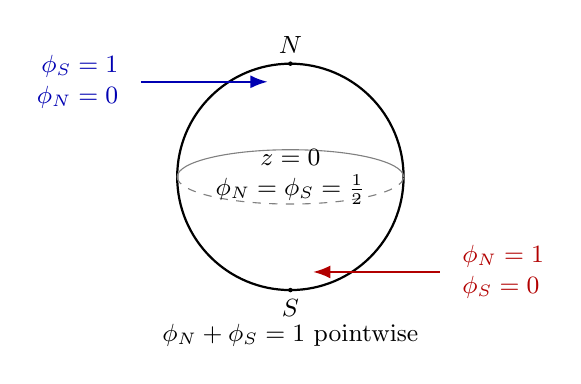
\begin{tikzpicture}[scale=1.15, every node/.style={font=\small}]
\draw[thick] (0,0) circle (1.25);
\draw[dashed, black!50] (-1.25,0) arc (180:360:1.25 and 0.3);
\draw[black!50] (1.25,0) arc (0:180:1.25 and 0.3);
\fill (0,1.25) circle (0.025) node[above] {$N$};
\fill (0,-1.25) circle (0.025) node[below] {$S$};
\draw[vector, blue!70!black] (-1.65,1.05) -- (-0.25,1.05);
\draw[vector, red!70!black] (1.65,-1.05) -- (0.25,-1.05);
\node[blue!70!black, align=right] at (-2.35,1.05) {$\phi_S=1$\\$\phi_N=0$};
\node[red!70!black, align=left] at (2.35,-1.05) {$\phi_N=1$\\$\phi_S=0$};
\node[align=center] at (0,0) {$z=0$\\$\phi_N=\phi_S=\frac12$};
\node[align=center] at (0,-1.75) {$\phi_N+\phi_S=1$ pointwise};
\end{tikzpicture}
\visualcaption{The two weights trade mass from north to south. Their symmetry explains why each weighted area integral contributes $2\pi$.}
\end{center}

\subsection*{Problem 8(a): Verifying the partition of unity}

\solutionflow{\(\phi_N=\frac{1-z}{2}\)\\\(\phi_S=\frac{1+z}{2}\)}
{nonnegative\\on \(-1\le z\le1\)}
{sum equals\\\(1\)}
{Problem 8(a) is solved by checking positivity and the pointwise sum on the sphere.}

On $S^2$, the coordinate $z$ satisfies
\[
 -1\leq z\leq1.
\]
Therefore
\[
 0\leq \frac{1-z}{2}\leq1,
 \qquad
 0\leq \frac{1+z}{2}\leq1.
\]
Also,
\[
 \phi_N+\phi_S
 =
 \frac{1-z}{2}+\frac{1+z}{2}
 =
 1.
\]
Finally,
\[
 \phi_N(0,0,1)=0,
 \qquad
 \phi_S(0,0,-1)=0.
\]
Thus $\phi_N$ vanishes at the north pole and $\phi_S$ vanishes at the south pole.

There is a small technical point in the problem statement. With the standard definition
\[
 \operatorname{supp}(\phi)=
 \overline{\{p:\phi(p)\neq0\}},
\]
these functions are not literally subordinate to the open cover $\{U_N,U_S\}$, because
\[
 \{\phi_N\neq0\}=S^2\setminus\{(0,0,1)\}
\]
has closure all of $S^2$. Hence the north pole is still in $\operatorname{supp}(\phi_N)$, and similarly the south pole is still in $\operatorname{supp}(\phi_S)$. So, strictly speaking,
\[
 \operatorname{supp}(\phi_N)\nsubseteq U_N,
 \qquad
 \operatorname{supp}(\phi_S)\nsubseteq U_S.
\]
If the intended meaning is the weaker chart-wise statement that $\phi_N$ vanishes at the point missing from $U_N$ and $\phi_S$ vanishes at the point missing from $U_S$, then the following computations are valid. To get a genuine subordinate partition of unity in the strict sense, one would replace these functions by bump-function versions whose supports stay a positive distance away from the excluded poles.
For the purpose of the integral in this problem, the weaker statement is enough because changing or omitting a single point does not change the value of an integral of a smooth area form.

\begin{center}
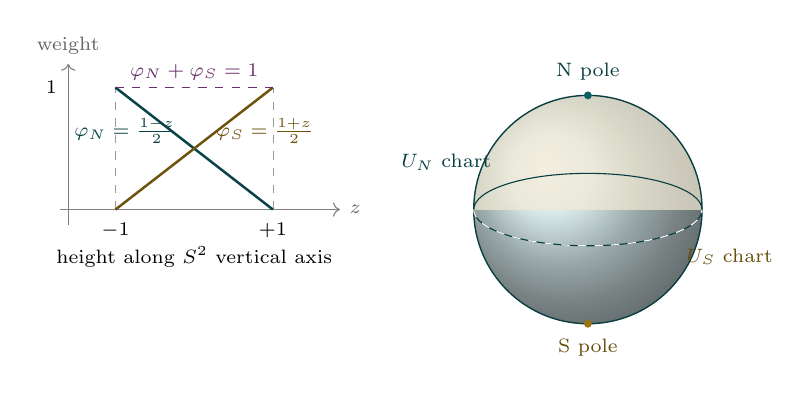
\begin{tikzpicture}[scale=1.0, every node/.style={font=\scriptsize}]
% Left: profile of phi_N and phi_S along z-axis (z from -1 to 1)
\begin{scope}
  \draw[->, black!50, line width=0.4pt] (-1.7,0) -- (1.85,0) node[right, black!60] {$z$};
  \draw[->, black!50, line width=0.4pt] (-1.6,-0.2) -- (-1.6,1.85) node[above, black!60] {weight};
  \draw[dashed, black!40, line width=0.3pt] (-1,0) -- (-1,1.55);
  \draw[dashed, black!40, line width=0.3pt] (1,0) -- (1,1.55);
  \node[font=\scriptsize, below] at (-1,-0.05) {$-1$};
  \node[font=\scriptsize, below] at (1,-0.05) {$+1$};
  \node[font=\scriptsize, left] at (-1.62,1.55) {$1$};
  % phi_N(z) = (1-z)/2 (linear)
  \draw[formteal!60!black, line width=0.9pt] (-1,1.55) -- (1,0);
  \node[formteal!60!black, font=\scriptsize, anchor=west] at (-1.65,1.0) {$\varphi_N=\tfrac{1-z}{2}$};
  % phi_S(z) = (1+z)/2 (linear)
  \draw[formgold!60!black, line width=0.9pt] (-1,0) -- (1,1.55);
  \node[formgold!60!black, font=\scriptsize, anchor=east] at (1.65,1.0) {$\varphi_S=\tfrac{1+z}{2}$};
  % horizontal at 1 (sum)
  \draw[dashed, formplum, line width=0.5pt] (-1,1.55) -- (1,1.55);
  \node[formplum, font=\scriptsize] at (0,1.75) {$\varphi_N+\varphi_S=1$};
  \node[font=\scriptsize] at (0,-0.6) {height along $S^2$ vertical axis};
\end{scope}
% Right: globe with two charts colored
\begin{scope}[xshift=5.0cm]
  \shade[ball color=formteal!25, opacity=0.85] (0,0) circle (1.45);
  % Upper hemisphere (phi_S large)
  \begin{scope}
    \clip (0,0) circle (1.45);
    \fill[formgold!18, opacity=0.7] (-1.5,0) rectangle (1.5,1.5);
  \end{scope}
  \draw[formteal!55!black, line width=0.5pt] (0,0) circle (1.45);
  \draw[formteal!55!black, line width=0.4pt] (0,0) ellipse (1.45 and 0.46);
  \draw[dashed, white, line width=0.4pt] (-1.45,0) arc (180:360:1.45 and 0.46);
  % North pole
  \fill[formteal!85!black] (0,1.45) circle (0.05);
  \node[formteal!55!black, font=\scriptsize, above] at (0,1.52) {N pole};
  % South pole
  \fill[formgold!85!black] (0,-1.45) circle (0.05);
  \node[formgold!55!black, font=\scriptsize, below] at (0,-1.52) {S pole};
  \node[formteal!55!black, font=\scriptsize] at (-1.8,0.6) {$U_N$ chart};
  \node[formgold!55!black, font=\scriptsize] at (1.8,-0.6) {$U_S$ chart};
\end{scope}
\end{tikzpicture}
\visualcaption{The partition functions $\varphi_N$ and $\varphi_S$ form a linear ``ramp'' along the height axis of the sphere. Each vanishes at one pole, lives in its corresponding chart, and the two add to the constant function $1$ on $S^2$.}
\end{center}

\subsection*{Problem 8(b): Local expressions in stereographic coordinates}

\solutionflow{insert formula\\for \(z(w)\)}
{compute\\\((1\mp z)/2\)}
{both charts give\\\(\frac{1}{1+|w|^2}\)}
{Problem 8(b) is solved by substituting the stereographic expression for the height coordinate.}

In the north stereographic coordinate $w=u+iv$, the problem gives
\[
 z=\frac{|w|^2-1}{|w|^2+1}.
\]
Then
\[
\begin{aligned}
 \phi_N
 &=
 \frac{1-z}{2}\\
 &=
 \frac12
 \left(
 1-\frac{|w|^2-1}{|w|^2+1}
 \right)\\
 &=
 \frac12
 \left(
 \frac{2}{1+|w|^2}
 \right)\\
 &=
 \frac{1}{1+|w|^2}.
\end{aligned}
\]
In the south stereographic coordinate, the problem gives
\[
 z=\frac{1-|w|^2}{1+|w|^2}.
\]
Then
\[
\begin{aligned}
 \phi_S
 &=
 \frac{1+z}{2}\\
 &=
 \frac12
 \left(
 1+\frac{1-|w|^2}{1+|w|^2}
 \right)\\
 &=
 \frac{1}{1+|w|^2}.
\end{aligned}
\]

\subsection*{Problem 8(c): Integrating one term of the partition}

\solutionflow{\(\phi_N dA\)}
{polar form\\\(\frac{4r}{(1+r^2)^3}\,dr\,d\theta\)}
{radial integral \(1\)\\so total \(2\pi\)}
{Problem 8(c) is solved by reducing the weighted area integral to a single radial integral.}

Using north stereographic coordinates,
\[
 dA=\frac{4}{(1+|w|^2)^2}\,du\,dv,
 \qquad
 \phi_N=\frac{1}{1+|w|^2}.
\]
Thus
\[
\begin{aligned}
 \int_{U_N}\phi_N\,dA
 &=
 \int_{\R^2}
 \frac{1}{1+|w|^2}
 \frac{4}{(1+|w|^2)^2}
 \,du\,dv\\
 &=
 \int_{\R^2}
 \frac{4}{(1+|w|^2)^3}
 \,du\,dv.
\end{aligned}
\]
Now use polar coordinates $w=re^{i\theta}$:
\[
 du\,dv=r\,dr\,d\theta.
\]
Then
\[
 \int_{U_N}\phi_N\,dA
 =
 \int_0^{2\pi}\int_0^\infty
 \frac{4r}{(1+r^2)^3}\,dr\,d\theta.
\]

\begin{center}
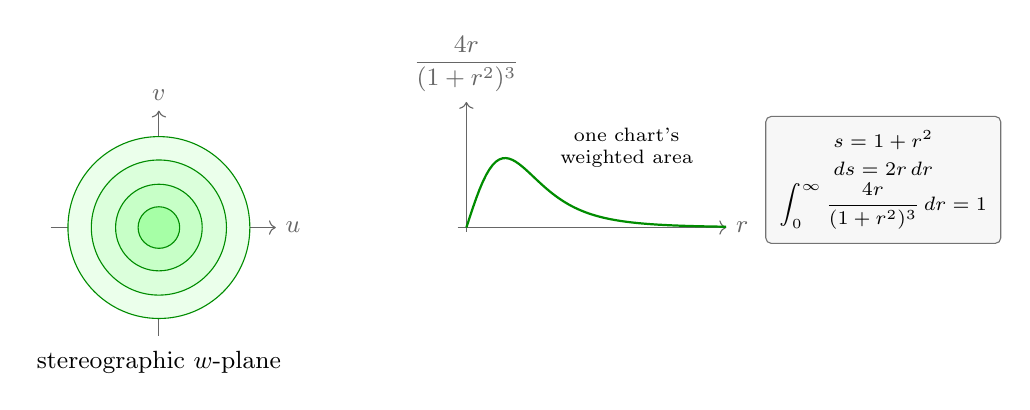
\begin{tikzpicture}[scale=1.1, every node/.style={font=\small}]
\begin{scope}
  \draw[->, black!60] (-1.25,0) -- (1.35,0) node[right] {$u$};
  \draw[->, black!60] (0,-1.25) -- (0,1.35) node[above] {$v$};
  \foreach \r/\c in {1.05/green!8,0.78/green!14,0.5/green!22,0.24/green!35}
    \filldraw[draw=green!55!black, fill=\c] (0,0) circle (\r);
  \node at (0,-1.55) {stereographic $w$-plane};
\end{scope}
\begin{scope}[xshift=3.55cm]
  \draw[->, black!60] (-0.1,0) -- (3.0,0) node[right] {$r$};
  \draw[->, black!60] (0,-0.05) -- (0,1.45) node[above] {$\dfrac{4r}{(1+r^2)^3}$};
  \draw[thick, green!55!black, domain=0:3, samples=80, variable=\r]
    plot ({\r},{3.1*\r/((1+\r*\r)*(1+\r*\r)*(1+\r*\r))});
  \node[font=\scriptsize, align=center] at (1.85,0.92) {one chart's\\weighted area};
\end{scope}
\node[visualnode, anchor=west, font=\scriptsize] at (7.0,0.55)
{$s=1+r^2$\\[2pt]
$ds=2r\,dr$\\[2pt]
$\displaystyle \int_0^\infty \frac{4r}{(1+r^2)^3}\,dr=1$};
\end{tikzpicture}
\visualcaption{After passing to polar coordinates in a stereographic chart, each partition term is one radial integral times the angular factor $2\pi$.}
\end{center}
Let $s=1+r^2$, so $ds=2r\,dr$. The radial integral is
\[
\begin{aligned}
 \int_0^\infty
 \frac{4r}{(1+r^2)^3}\,dr
 &=
 2\int_1^\infty s^{-3}\,ds\\
 &=
 2\left[-\frac{1}{2s^2}\right]_1^\infty\\
 &=
 1.
\end{aligned}
\]
Therefore
\[
 \int_{U_N}\phi_N\,dA
 =
 \int_0^{2\pi}1\,d\theta
 =
 2\pi.
\]
It is useful to check the size of the integral before trusting the answer. Since $\phi_N=(1-z)/2$, it is larger near the south pole and smaller near the north pole. By symmetry the complementary function $\phi_S=(1+z)/2$ should contribute the same total amount, so each term should be half of the total area $4\pi$, namely $2\pi$.

\subsection*{Problem 8(d): Integrating the second term}

\solutionflow{south chart\\same formulas}
{same polar integral}
{same result\\\(2\pi\)}
{Problem 8(d) is solved by symmetry: the south-chart weighted integral repeats the north-chart computation.}

The south chart gives the same local formulas:
\[
 \phi_S=\frac{1}{1+|w|^2},
 \qquad
 dA=\frac{4}{(1+|w|^2)^2}\,du\,dv.
\]
Therefore the integral is the same as in part (c):
\[
 \int_{U_S}\phi_S\,dA
 =
 \int_{\R^2}
 \frac{4}{(1+|w|^2)^3}
 \,du\,dv
 =
 2\pi.
\]

\subsection*{Problem 8(e): Recovering the total area of the sphere}

\solutionflow{\(\phi_N+\phi_S=1\)}
{integrate termwise}
{\(2\pi+2\pi=4\pi\)}
{Problem 8(e) is solved by adding the two partition-of-unity contributions.}

Since
\[
 \phi_N+\phi_S=1,
\]
we have
\[
 \int_{S^2}dA
 =
 \int_{U_N}\phi_N\,dA
 +
 \int_{U_S}\phi_S\,dA.
\]
Using parts (c) and (d),
\[
 \int_{S^2}dA
 =
 2\pi+2\pi
 =
 4\pi.
\]
Thus
\[
 \operatorname{Area}(S^2)=4\pi.
\]

\section*{Problem 9: Mayer--Vietoris Sequence and de Rham Cohomology}

\begin{intentrequirements}
\item \textbf{Intent.} Build the Mayer--Vietoris long exact sequence in de Rham cohomology from a short exact sequence of differential-form complexes.
\item \textbf{Required outputs.} Prove exactness of
\[
 0\to\Om^k(M)\to\Om^k(U)\oplus\Om^k(V)\to\Om^k(U\cap V)\to0,
\]
show compatibility with the exterior derivative, construct the connecting homomorphism, explain the Snake Lemma input, and write the resulting long exact sequence.
\item \textbf{Required explanations.} Interpret the maps geometrically: $i$ restricts a global form to $U$ and $V$, while $\rho$ measures the difference of two local forms on the overlap. Exactness at the middle term is precisely the gluing condition.
\item \textbf{Common pitfalls to avoid.} The connecting homomorphism raises degree by one because it differentiates local lifts. The result is a cohomology class, so the proof must explain why different choices of representative and lift change the glued form only by an exact form.
\end{intentrequirements}

\windingnote{The winding form $\omega$ is the canonical generator of $H^1(\R^2\setminus\{0\})\cong\R$, and Mayer--Vietoris constructs that class explicitly. Cover the punctured plane by $U=\R^2\setminus\{(-\infty,0]\}$ (slit at the negative $x$-axis) and $V=\R^2\setminus\{[0,\infty)\}$ (slit at the positive $x$-axis); both are simply connected, so $H^1(U)=H^1(V)=0$, while $U\cap V$ is the union of the upper and lower half-planes, two contractible pieces with $H^0(U\cap V)=\R^2$. The Mayer--Vietoris long exact sequence then gives
\[
 0\to H^0(\R^2\!\setminus\!\{0\})\to H^0(U)\oplus H^0(V)\to H^0(U\cap V)\xrightarrow{\delta}H^1(\R^2\!\setminus\!\{0\})\to 0,
\]
forcing $H^1(\R^2\!\setminus\!\{0\})\cong\R$. The connecting map $\delta$ constructed in Problem~9(c) takes the locally constant function $1$ on the upper half-overlap (and $0$ on the lower) and lifts it to local $\arg$-branches on $U$ and $V$ whose differentials disagree on the overlap by the constant $2\pi$ --- which then \emph{glues to $\omega$ itself}. Thus the winding form is not just an example; it is the universal output of $\delta$ on the simplest non-trivial punctured surface.}

\handsketch{%
\fill[handpaper] (-3.4,-1.9) rectangle (3.4,1.9);
\draw[hand] (-3.4,-1.9) rectangle (3.4,1.9);
% Punctured plane outline
\draw[handthick] (-2.6,-1.4) rectangle (2.6,1.4);
% Origin puncture
\fill[handink] (0,0) circle (0.07);
\draw[handthick] (0,0) circle (0.18);
% Slit along negative x-axis (U-slit)
\draw[draw=handink, dashed, line width=0.5pt] (-2.5,0) -- (-0.18,0);
\node[handnote] at (-2.0,0.25) {slit for $U$};
% Slit along positive x-axis (V-slit)
\draw[draw=handink, dashed, line width=0.5pt] (0.18,0) -- (2.5,0);
\node[handnote] at (2.0,-0.25) {slit for $V$};
% Overlap regions: upper and lower half-planes
\node[handnote] at (-1.4,0.85) {$U\cap V$ upper};
\node[handnote] at (1.4,-0.85) {$U\cap V$ lower};
% delta arrow
\node[handnote] at (1.95,1.55) {$\delta(1_{\text{upper}})=[\omega]$};
\node[handnote] at (-1.95,-1.55) {$H^1\cong\R\langle[\omega]\rangle$};
}

Let $M=U\cup V$ be an open cover. For each degree $k$, define
\[
 i:\Om^k(M)\to \Om^k(U)\oplus\Om^k(V),
 \qquad
 i(\omega)=(\omega|_U,\omega|_V),
\]
and
\[
 \rho:\Om^k(U)\oplus\Om^k(V)\to \Om^k(U\cap V),
 \qquad
 \rho(\alpha,\beta)=\alpha|_{U\cap V}-\beta|_{U\cap V}.
\]

\begin{center}
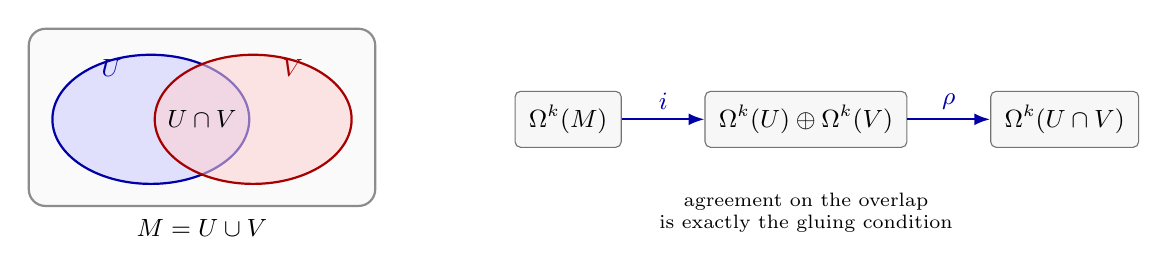
\begin{tikzpicture}[scale=1.0, every node/.style={font=\small}]
\begin{scope}
  \draw[rounded corners=6pt, thick, black!45, fill=black!2] (-2.2,-1.1) rectangle (2.2,1.15);
  \filldraw[draw=blue!65!black, fill=blue!20, fill opacity=0.55, thick] (-0.65,0) ellipse (1.25 and 0.82);
  \filldraw[draw=red!65!black, fill=red!18, fill opacity=0.55, thick] (0.65,0) ellipse (1.25 and 0.82);
  \node[blue!65!black] at (-1.15,0.65) {$U$};
  \node[red!65!black] at (1.15,0.65) {$V$};
  \node at (0,0) {$U\cap V$};
  \node at (0,-1.38) {$M=U\cup V$};
\end{scope}
\begin{scope}[xshift=4.65cm]
  \node[visualnode] (m) {$\Omega^k(M)$};
  \node[visualnode, right=1.05cm of m] (uv) {$\Omega^k(U)\oplus\Omega^k(V)$};
  \node[visualnode, right=1.05cm of uv] (int) {$\Omega^k(U\cap V)$};
  \draw[formarrow] (m) -- node[above] {$i$} (uv);
  \draw[formarrow] (uv) -- node[above] {$\rho$} (int);
  \node[font=\scriptsize, align=center, below=0.45cm of uv] {agreement on the overlap\\is exactly the gluing condition};
\end{scope}
\end{tikzpicture}
\visualcaption{The map $i$ restricts a global form to the two open sets. The map $\rho$ measures the mismatch of two local forms on the overlap.}
\end{center}

\subsection*{Problem 9(a): Short exact sequence of differential forms}

\solutionflow{restrict\\global forms}
{measure mismatch\\on \(U\cap V\)}
{partition of unity\\proves surjectivity}
{Problem 9(a) is solved by interpreting exactness as gluing plus a partition-of-unity construction.}

We show that
\[
 0\to\Om^k(M)
 \xrightarrow{i}
 \Om^k(U)\oplus\Om^k(V)
 \xrightarrow{\rho}
 \Om^k(U\cap V)
 \to0
\]
is exact.

First, $i$ is injective. If
\[
 i(\omega)=(0,0),
\]
then
\[
 \omega|_U=0,
 \qquad
 \omega|_V=0.
\]
Since $U\cup V=M$, the form $\omega$ is zero everywhere on $M$. Hence $\omega=0$.

Next, we compute $\ker\rho$. Suppose
\[
 \rho(\alpha,\beta)=0.
\]
Then
\[
 \alpha|_{U\cap V}=\beta|_{U\cap V}.
\]
So $\alpha$ and $\beta$ agree on the overlap. Therefore they glue to a unique global $k$-form $\omega\in\Om^k(M)$ such that
\[
 \omega|_U=\alpha,
 \qquad
 \omega|_V=\beta.
\]
Thus
\[
 (\alpha,\beta)=i(\omega),
\]
so
\[
 \ker\rho=\operatorname{im}i.
\]

Finally, $\rho$ is surjective. Let
\[
 \gamma\in\Om^k(U\cap V).
\]
Choose a partition of unity $\{\varphi_U,\varphi_V\}$ subordinate to the cover $\{U,V\}$. Define
\[
 \alpha=\varphi_V\gamma\quad\text{on }U,
 \qquad
 \beta=-\varphi_U\gamma\quad\text{on }V.
\]
More explicitly, $\varphi_V\gamma$ is only needed on the part of $U$ where $\varphi_V$ is supported; that support lies in $V$, so it lies in $U\cap V$ when restricted to $U$. This is what makes the expression meaningful and smooth. Similarly, $-\varphi_U\gamma$ is meaningful on $V$. These forms are extended by zero where needed, smoothly, because the supports are subordinate to the cover. On $U\cap V$,
\[
\begin{aligned}
 \rho(\alpha,\beta)
 &=
 \alpha-\beta\\
 &=
 \varphi_V\gamma+\varphi_U\gamma\\
 &=
 (\varphi_U+\varphi_V)\gamma\\
 &=
 \gamma.
\end{aligned}
\]
Thus $\rho$ is surjective. This proves exactness at every term, so the sequence is short exact.

\subsection*{Problem 9(b): Compatibility with the exterior derivative}

\solutionflow{restriction maps}
{commute with\\\(d\)}
{short exact sequence\\of complexes}
{Problem 9(b) is solved by using the locality of exterior differentiation.}

Restriction commutes with exterior differentiation. For every form $\omega$,
\[
 (d\omega)|_U=d(\omega|_U),
 \qquad
 (d\omega)|_V=d(\omega|_V).
\]
The same is true after restricting to $U\cap V$. Hence the maps $i$ and $\rho$ commute with $d$:
\[
 i(d\omega)=d(i\omega),
 \qquad
 \rho(d\alpha,d\beta)=d(\rho(\alpha,\beta)).
\]
Therefore the short exact sequence above is a short exact sequence of cochain complexes:
\[
 0\to\Om^\bullet(M)
 \to
 \Om^\bullet(U)\oplus\Om^\bullet(V)
 \to
 \Om^\bullet(U\cap V)
 \to0.
\]

\subsection*{Problem 9(c): Constructing the connecting homomorphism}

\solutionflow{closed overlap class\\\([\gamma]\)}
{choose local lift\\\((\alpha,\beta)\)}
{differentiate and glue\\to \(\delta[\gamma]\)}
{Problem 9(c) is solved by differentiating local lifts and using exactness to glue the result.}

Let
\[
 [\gamma]\in H^k(U\cap V)
\]
be a cohomology class, and choose a closed representative
\[
 d\gamma=0.
\]
Because $\rho$ is surjective, choose a lift
\[
 (\alpha,\beta)\in\Om^k(U)\oplus\Om^k(V)
\]
such that
\[
 \rho(\alpha,\beta)=\gamma.
\]
That is,
\[
 \alpha|_{U\cap V}-\beta|_{U\cap V}=\gamma.
\]
Now apply $d$:
\[
 d\alpha|_{U\cap V}-d\beta|_{U\cap V}=d\gamma=0.
\]
So $d\alpha$ and $d\beta$ agree on $U\cap V$. Therefore they glue to a global $(k+1)$-form
\[
 \omega\in\Om^{k+1}(M)
\]
with
\[
 \omega|_U=d\alpha,
 \qquad
 \omega|_V=d\beta.
\]
This form is closed because locally it is an exterior derivative and $d^2=0$:
\[
 d\omega|_U=d^2\alpha=0,
 \qquad
 d\omega|_V=d^2\beta=0.
\]
Define
\[
 \delta([\gamma])=[\omega]\in H^{k+1}(M).
\]

\begin{center}
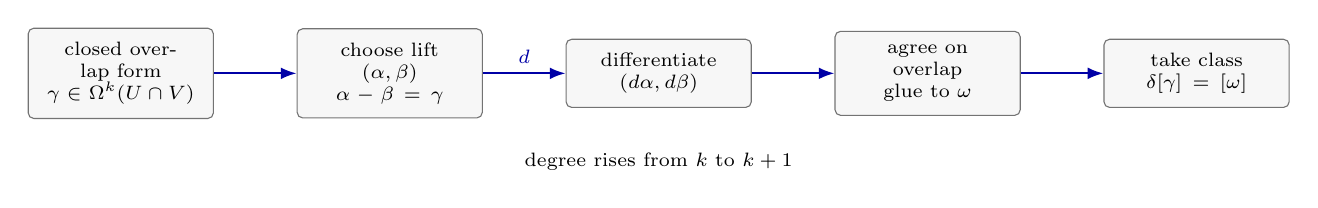
\begin{tikzpicture}[node distance=1.05cm, every node/.style={font=\scriptsize}]
\node[visualnode, text width=2.0cm] (gamma) {closed overlap form\\$\gamma\in\Omega^k(U\cap V)$};
\node[visualnode, text width=2.0cm, right=of gamma] (lift) {choose lift\\$(\alpha,\beta)$\\$\alpha-\beta=\gamma$};
\node[visualnode, text width=2.0cm, right=of lift] (diff) {differentiate\\$(d\alpha,d\beta)$};
\node[visualnode, text width=2.0cm, right=of diff] (glue) {agree on overlap\\glue to $\omega$};
\node[visualnode, text width=2.0cm, right=of glue] (class) {take class\\$\delta[\gamma]=[\omega]$};
\draw[formarrow] (gamma) -- (lift);
\draw[formarrow] (lift) -- node[above] {$d$} (diff);
\draw[formarrow] (diff) -- (glue);
\draw[formarrow] (glue) -- (class);
\node[below=0.45cm of diff, align=center, font=\scriptsize] {degree rises from $k$ to $k+1$};
\end{tikzpicture}
\visualcaption{The connecting homomorphism is a controlled failure-to-lift construction: lift locally, differentiate, glue, then pass to cohomology.}
\end{center}
One must check that this does not depend on the chosen representative $\gamma$ or on the chosen lift $(\alpha,\beta)$.

First suppose we choose a different lift of the same $\gamma$. The difference of two lifts lies in $\ker\rho$, so by exactness it comes from a global $k$-form on $M$. Applying $d$ changes the glued $(k+1)$-form by an exact form. Therefore the cohomology class does not change.

Second, if we replace $\gamma$ by a cohomologous representative $\gamma+d\tau$, then a compatible change of lift changes the glued form by an exact form again. Hence the class $[\omega]\in H^{k+1}(M)$ is well-defined.

\begin{center}
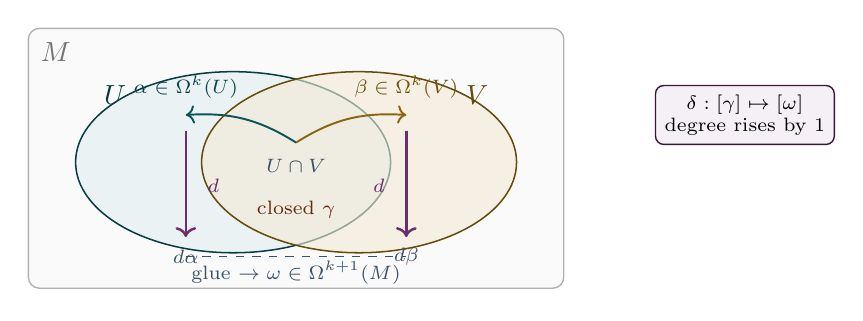
\begin{tikzpicture}[scale=1.0, every node/.style={font=\scriptsize}]
% Background space M = U ∪ V
\filldraw[draw=black!30, fill=black!2, line width=0.5pt, rounded corners=4pt]
  (-3.4,-1.6) rectangle (3.4,1.7);
\node[font=\bfseries, black!55] at (-3.05,1.4) {$M$};
% U (teal blob)
\filldraw[draw=formteal!55!black, fill=formteal!12, line width=0.55pt, fill opacity=0.6]
  (-0.8,0) ellipse (2.0 and 1.15);
\node[formteal!55!black, font=\bfseries] at (-2.3,0.85) {$U$};
% V (gold blob)
\filldraw[draw=formgold!55!black, fill=formgold!18, line width=0.55pt, fill opacity=0.6]
  (0.8,0) ellipse (2.0 and 1.15);
\node[formgold!55!black, font=\bfseries] at (2.3,0.85) {$V$};
% Overlap shading
\node[formslate, font=\scriptsize] at (0,-0.05) {$U\cap V$};
% Closed form on overlap: γ
\node[formrust!60!black, font=\scriptsize] at (0,-0.6) {closed $\gamma$};
% Arrows showing lift α, β
\draw[->, formteal!75!black, line width=0.7pt] (0.0,0.25) to[bend right=18] (-1.4,0.6);
\node[formteal!60!black, font=\scriptsize] at (-1.4,0.95) {$\alpha\in\Omega^k(U)$};
\draw[->, formgold!75!black, line width=0.7pt] (0.0,0.25) to[bend left=18] (1.4,0.6);
\node[formgold!60!black, font=\scriptsize] at (1.4,0.95) {$\beta\in\Omega^k(V)$};
% Differentiate
\draw[->, formplum, line width=0.9pt] (-1.4,0.4) -- (-1.4,-0.95);
\draw[->, formplum, line width=0.9pt] (1.4,0.4) -- (1.4,-0.95);
\node[formplum, font=\scriptsize] at (-1.05,-0.3) {$d$};
\node[formplum, font=\scriptsize] at (1.05,-0.3) {$d$};
% dα and dβ agree on overlap, glue
\node[formslate, font=\scriptsize] at (-1.4,-1.2) {$d\alpha$};
\node[formslate, font=\scriptsize] at (1.4,-1.2) {$d\beta$};
\draw[dashed, formslate, line width=0.5pt] (-1.4,-1.2) -- (1.4,-1.2);
\node[formslate, font=\scriptsize] at (0,-1.4) {glue $\to\omega\in\Omega^{k+1}(M)$};
% Caption box
\node[draw=formplum!50!black, fill=formplum!7, rounded corners=3pt, line width=0.5pt,
      align=center, font=\scriptsize] at (5.7,0.6)
      {$\delta:[\gamma]\mapsto[\omega]$\\degree rises by 1};
\end{tikzpicture}
\visualcaption{The connecting map cannot lift a closed overlap form globally in one step. It lifts locally to $(\alpha,\beta)$, differentiates them, and observes that the two pieces $d\alpha$, $d\beta$ now \emph{do} agree on the overlap — so they glue to a closed global form one degree higher.}
\end{center}

\subsection*{Problem 9(d): The Snake Lemma and the long exact sequence}

\solutionflow{two exact rows\\linked by \(d\)}
{Snake Lemma\\creates \(\delta\)}
{cohomology sequence\\continues}
{Problem 9(d) is solved by recognizing the standard Snake Lemma diagram behind the connecting map.}

At each degree $k$, we have a commutative diagram with exact rows:
\[
\begin{array}{ccccccccc}
0&\to&\Om^k(M)&\to&\Om^k(U)\oplus\Om^k(V)&\to&\Om^k(U\cap V)&\to&0\\
 &&\downarrow d&&\downarrow d&&\downarrow d&&\\
0&\to&\Om^{k+1}(M)&\to&\Om^{k+1}(U)\oplus\Om^{k+1}(V)&\to&\Om^{k+1}(U\cap V)&\to&0.
\end{array}
\]
The Snake Lemma is the algebraic tool that produces a connecting map from such a diagram. In this setting, it produces the same map described in part (c):
\[
 \delta:H^k(U\cap V)\to H^{k+1}(M).
\]
Conceptually, the map measures the obstruction to lifting a closed form on the overlap to compatible closed forms on $U$ and $V$.
If the obstruction vanishes, then the local choices can be corrected so that they glue in cohomology. If it does not vanish, the failure is recorded as a global cohomology class one degree higher.

\subsection*{Problem 9(e): Applying the Snake Lemma to the de Rham complex}

\solutionflow{short exact\\sequence of complexes}
{pass to\\closed modulo exact}
{long exact\\de Rham sequence}
{Problem 9(e) is solved by applying the homological algebra result degree by degree to the de Rham complexes.}

Because
\[
 0\to\Om^\bullet(M)
 \to
 \Om^\bullet(U)\oplus\Om^\bullet(V)
 \to
 \Om^\bullet(U\cap V)
 \to0
\]
is a short exact sequence of complexes, homological algebra gives a long exact sequence in cohomology. The kernels of $d$ are closed forms, and quotienting by images of $d$ means passing from closed forms to cohomology classes. Thus the Snake Lemma construction naturally descends to de Rham cohomology.
The word ``long'' means that the sequence continues through every degree. The maps preserve degree except for the connecting homomorphism $\delta$, which raises degree by one:
\[
 \delta:H^k(U\cap V)\to H^{k+1}(M).
\]
That degree shift is exactly why the sequence links the degree-$k$ terms to the degree-$(k+1)$ terms.

\subsection*{Problem 9(f): The Mayer--Vietoris long exact sequence}

\solutionflow{restriction map}
{difference on overlap}
{connecting map\\raises degree}
{Problem 9(f) is solved by writing the long exact sequence with the maps induced by restriction, difference, and \(\delta\).}

The resulting Mayer--Vietoris sequence is
\[
 \cdots
 \to H^k(M)
 \to H^k(U)\oplus H^k(V)
 \to H^k(U\cap V)
 \xrightarrow{\delta}
 H^{k+1}(M)
 \to H^{k+1}(U)\oplus H^{k+1}(V)
 \to\cdots.
\]
The first map is induced by restriction:
\[
 [\omega]\longmapsto([\omega|_U],[\omega|_V]).
\]
The second map subtracts the two restrictions to the overlap:
\[
 ([\alpha],[\beta])
 \longmapsto
 [\alpha|_{U\cap V}-\beta|_{U\cap V}].
\]
Exactness says that a class on one term maps to zero precisely when it came from the previous term. This is the cohomological version of the gluing principle used in part (a).
The logical structure is
\[
\begin{gathered}
 \text{short exact sequence of complexes}
 \Longrightarrow
 \text{connecting homomorphism}\\
 \Longrightarrow
 \text{long exact sequence in cohomology}.
\end{gathered}
\]
This is the Mayer--Vietoris long exact sequence for de Rham cohomology.

\section*{Additional Extremely Detailed Notes, Keyed by Problem Number}

This final section is intentionally redundant. Its purpose is to spell out the background algebra and geometry behind the computations above, so that each answer can be reconstructed from first principles.

\subsection*{Extra detail for Problem 1}

The most important sign rule is
\[
 \alpha\wedge\beta=(-1)^{kl}\beta\wedge\alpha
\]
when $\alpha$ is a $k$-form and $\beta$ is an $l$-form. For $1$-forms this says
\[
 dx\wedge dy=-dy\wedge dx,\qquad
 dy\wedge dz=-dz\wedge dy,\qquad
 dz\wedge dx=-dx\wedge dz.
\]
It also says
\[
 dx\wedge dx=dy\wedge dy=dz\wedge dz=0.
\]
These zero identities are the reason only certain terms survive when differentiating a $1$-form or a $2$-form.

For the curl computation, a useful memory device is:
\[
\begin{array}{c|c}
\text{component of curl} & \text{matching }2\text{-form}\\ \hline
(\nabla\times F)_1 & dy\wedge dz\\
(\nabla\times F)_2 & dz\wedge dx\\
(\nabla\times F)_3 & dx\wedge dy
\end{array}
\]
So after computing $d\omega$, do not read the coefficients in the order
$dx\wedge dy$, $dy\wedge dz$, $dz\wedge dx$. Instead read them in the vector-field order
\[
 dy\wedge dz,\quad dz\wedge dx,\quad dx\wedge dy.
\]

For the divergence computation, every surviving term becomes a multiple of the volume form
\[
 dx\wedge dy\wedge dz.
\]
For example,
\[
 dy\wedge dz\wedge dx=dx\wedge dy\wedge dz
\]
because moving $dx$ from the end to the front takes two swaps:
\[
 dy\wedge dz\wedge dx
 =
 -dy\wedge dx\wedge dz
 =
 dx\wedge dy\wedge dz.
\]
Likewise,
\[
 dz\wedge dx\wedge dy=dx\wedge dy\wedge dz.
\]
That is why the divergence has plus signs:
\[
 \pd_xF_1+\pd_yF_2+\pd_zF_3.
\]

\subsection*{Extra detail for Problem 2}

When integrating a $1$-form over a parameterized curve $\gamma(t)=(x(t),y(t))$, the actual operation is pullback:
\[
 \int_\gamma \omega=\int_a^b \gamma^*\omega.
\]
If
\[
 \omega=P(x,y)\,dx+Q(x,y)\,dy,
\]
then
\[
 \gamma^*\omega
 =
 P(x(t),y(t))x'(t)\,dt
 +
 Q(x(t),y(t))y'(t)\,dt.
\]
For the winding form on $S^1$,
\[
 P=-y,\qquad Q=x.
\]
With $x=\cos\theta$ and $y=\sin\theta$,
\[
 x'(\theta)=-\sin\theta,\qquad y'(\theta)=\cos\theta.
\]
So
\[
 P x'+Q y'
 =
 (-\sin\theta)(-\sin\theta)+(\cos\theta)(\cos\theta)
 =
 1.
\]
That is the fully expanded reason the pullback is $d\theta$.

The semicircle method is more delicate only because $x$ is not a global coordinate on the circle. On the upper semicircle, counterclockwise motion means
\[
 (1,0)\to(0,1)\to(-1,0),
\]
so $x$ decreases from $1$ to $-1$. On the lower semicircle, counterclockwise motion means
\[
 (-1,0)\to(0,-1)\to(1,0),
\]
so $x$ increases from $-1$ to $1$. These orientation facts are exactly what make both integrals positive.

\subsection*{Extra detail for Problem 3}

The Cauchy--Green proof has three independent sign sources:
\begin{enumerate}
\item the inner boundary orientation;
\item the wedge-product identity $d\bar\omega\wedge d\omega=-d\omega\wedge d\bar\omega$;
\item the factor $2\pi i$ from the positively oriented small circle.
\end{enumerate}
Keeping these separate prevents most mistakes.

Let $\omega=\xi+i\eta$. Then
\[
 d\omega=d\xi+i\,d\eta,\qquad d\bar\omega=d\xi-i\,d\eta.
\]
Expanding gives
\[
\begin{aligned}
 d\bar\omega\wedge d\omega
 &=(d\xi-i\,d\eta)\wedge(d\xi+i\,d\eta)\\
 &=i\,d\xi\wedge d\eta-i\,d\eta\wedge d\xi\\
 &=2i\,d\xi\wedge d\eta.
\end{aligned}
\]
Similarly,
\[
 d\omega\wedge d\bar\omega=-2i\,d\xi\wedge d\eta.
\]
Thus changing the order of $d\omega$ and $d\bar\omega$ changes the sign.

The small circle computation is just the residue computation written without invoking the residue theorem:
\[
 \omega=z+\eps e^{it},\qquad d\omega=i\eps e^{it}\,dt.
\]
Then
\[
 \frac{d\omega}{\omega-z}
 =
 \frac{i\eps e^{it}\,dt}{\eps e^{it}}
 =
 i\,dt.
\]
If $f(\omega)$ were exactly constant and equal to $f(z)$ on the circle, the integral would immediately be
\[
 \int_0^{2\pi} i f(z)\,dt=2\pi i f(z).
\]
Continuity of $f$ says that as $\eps\to0$, $f(z+\eps e^{it})$ becomes uniformly close to $f(z)$, so the same limit holds.

\subsection*{Extra detail for Problem 4}

All four theorems in Problem 4 have the same pattern:
\[
 \int_{\partial(\text{region})}\text{form}
 =
 \int_{\text{region}}d(\text{form}).
\]
The classical names differ because the degree of the form and the dimension of the region differ.

For the line-integral theorem, the region is the interval $[0,1]$ and its boundary is the signed pair
\[
 \partial[0,1]=\{1\}-\{0\}.
\]
So Stokes' theorem says
\[
 \int_{[0,1]}d(f\circ\gamma)
 =
 f(\gamma(1))-f(\gamma(0)).
\]
This is the ordinary fundamental theorem of calculus in disguise.

For Green's theorem, the region is a planar domain $D$ and the form is
\[
 \omega=P\,dx+Q\,dy.
\]
Then
\[
 d\omega=dP\wedge dx+dQ\wedge dy.
\]
Writing
\[
 dP=P_xdx+P_y dy,\qquad dQ=Q_xdx+Q_y dy,
\]
we get
\[
 dP\wedge dx=P_y\,dy\wedge dx=-P_y\,dx\wedge dy,
\]
and
\[
 dQ\wedge dy=Q_x\,dx\wedge dy.
\]
Therefore
\[
 d\omega=(Q_x-P_y)\,dx\wedge dy,
\]
which is exactly Green's theorem.

\subsection*{Extra detail for Problem 5}

The expression
\[
 \frac{\pd f}{\pd\bar z}
 =
 \frac12\left((u_x-v_y)+i(v_x+u_y)\right)
\]
contains both Cauchy--Riemann equations at once. The real part is
\[
 \frac12(u_x-v_y),
\]
so setting it to zero gives
\[
 u_x=v_y.
\]
The imaginary part is
\[
 \frac12(v_x+u_y),
\]
so setting it to zero gives
\[
 v_x=-u_y,
\]
or equivalently
\[
 u_y=-v_x.
\]

The Cauchy Integral Theorem proof in the problem is a good example of converting a complex statement into two real statements. If
\[
 \oint_{\partial D}f(z)\,dz=A+iB,
\]
then proving the complex integral is zero means proving
\[
 A=0,\qquad B=0.
\]
Green's theorem gives
\[
 A=\iint_D(-v_x-u_y)\,dx\,dy,
\]
and
\[
 B=\iint_D(u_x-v_y)\,dx\,dy.
\]
The Cauchy--Riemann equations make both integrands identically zero, so both integrals vanish.

\subsection*{Extra detail for Problem 6}

For a parameterized surface $X(u,v)$, the vectors $X_u$ and $X_v$ span the tangent plane. The first fundamental form records their dot products:
\[
 E=\langle X_u,X_u\rangle,\qquad
 F=\langle X_u,X_v\rangle,\qquad
 G=\langle X_v,X_v\rangle.
\]
The area of the parallelogram spanned by $X_u$ and $X_v$ is
\[
 \|X_u\times X_v\|.
\]
The identity
\[
 \|X_u\times X_v\|^2=EG-F^2
\]
explains the formula
\[
 dA=\sqrt{EG-F^2}\,du\,dv.
\]

The second fundamental form measures how the surface bends in the normal direction:
\[
 e=\langle X_{uu},N\rangle,\qquad
 f=\langle X_{uv},N\rangle,\qquad
 g=\langle X_{vv},N\rangle.
\]
The Gaussian curvature is the ratio
\[
 K=\frac{\det(\text{second fundamental form})}{\det(\text{first fundamental form})}
 =
 \frac{eg-f^2}{EG-F^2}.
\]
For the sphere, both determinants are $\sin^2\phi$, so $K=1$. For the torus, the determinant changes sign depending on $\cos u$, so the curvature is positive on the outer side and negative on the inner side.

\subsection*{Extra detail for Problem 7}

The metric
\[
 ds^2=\frac{4}{(1+|z|^2)^2}|dz|^2
\]
is the round metric on the sphere written in stereographic coordinates. The factor
\[
 \lambda=\frac{4}{(1+|z|^2)^2}
\]
shrinks lengths far away from the origin in the $z$-plane. This is why the whole noncompact plane $\C$ represents a compact sphere with finite total area.

The area integral
\[
 \int_{\C}\frac{4}{(1+|z|^2)^2}\,dx\,dy
\]
becomes, in polar coordinates,
\[
 \int_0^{2\pi}\int_0^\infty\frac{4r}{(1+r^2)^2}\,dr\,d\theta.
\]
The substitution $s=1+r^2$ gives $ds=2r\,dr$, so
\[
 \int_0^\infty\frac{4r}{(1+r^2)^2}\,dr
 =
 2\int_1^\infty s^{-2}\,ds
 =
 2\left[-s^{-1}\right]_1^\infty
 =
 2.
\]
Multiplying by the angular integral $2\pi$ gives $4\pi$.

\subsection*{Extra detail for Problem 8}

In stereographic coordinates, the sphere's area form is
\[
 dA=\frac{4}{(1+|w|^2)^2}\,du\,dv.
\]
The partition functions become
\[
 \phi_N=\frac{1}{1+|w|^2},
 \qquad
 \phi_S=\frac{1}{1+|w|^2}
\]
in their respective charts. Therefore each integral has the same radial form:
\[
 \int_{\R^2}\frac{4}{(1+|w|^2)^3}\,du\,dv.
\]
In polar coordinates,
\[
 du\,dv=r\,dr\,d\theta,
\]
so
\[
 \int_{\R^2}\frac{4}{(1+|w|^2)^3}\,du\,dv
 =
 \int_0^{2\pi}\int_0^\infty\frac{4r}{(1+r^2)^3}\,dr\,d\theta.
\]
With $s=1+r^2$,
\[
 \int_0^\infty\frac{4r}{(1+r^2)^3}\,dr
 =
 2\int_1^\infty s^{-3}\,ds
 =
 1.
\]
Thus each partition term contributes $2\pi$.

\subsection*{Extra detail for Problem 9}

Exactness of
\[
 0\to\Om^k(M)\xrightarrow{i}\Om^k(U)\oplus\Om^k(V)\xrightarrow{\rho}\Om^k(U\cap V)\to0
\]
means three things:
\begin{enumerate}
\item $i$ has no kernel except zero.
\item The image of $i$ is exactly the kernel of $\rho$.
\item $\rho$ is onto.
\end{enumerate}
The middle statement is the most geometric one. It says that a pair of forms $(\alpha,\beta)$ on $U$ and $V$ comes from a single global form on $M$ exactly when the two forms agree on the overlap $U\cap V$.

The connecting homomorphism has the following logic:
\[
\begin{gathered}
 \text{closed form on overlap}
 \to
 \text{choose local lifts}
 \to
 \text{differentiate the lifts}\\
 \to
 \text{glue the derivatives}
 \to
 \text{global cohomology class}.
\end{gathered}
\]
The degree goes up by one because we differentiate the chosen $k$-forms $\alpha,\beta$, producing $(k+1)$-forms $d\alpha,d\beta$.

The reason the glued derivative is closed is local:
\[
 d(d\alpha)=0\quad\text{on }U,
\qquad
 d(d\beta)=0\quad\text{on }V.
\]
Since $U\cup V=M$, this proves the global form is closed. The reason only the cohomology class matters is that different choices of lifts change the glued derivative by an exact form.

\end{document}
